\documentclass{article}

% packages
\usepackage{amsmath, amsthm, thmtools, amsfonts, amssymb, luacode, catchfile, tikzducks, hyperref, ifthen}
\ifcsname c@kobocompile\endcsname
	\usepackage[a5paper, total={1072pt, 1448pt}, margin=10pt, includeheadfoot]{geometry} % set page margins
\else
	\usepackage[a4paper, margin=50pt, includeheadfoot]{geometry}
\fi
\usepackage[shortlabels]{enumitem}
\usepackage[skip=3pt, indent=0pt]{parskip}

% language
\usepackage[bidi=basic, layout=tabular, provide=*]{babel}
\ifcsname c@english\endcsname
	\babelprovide[main, import]{english}
\else
	\babelprovide[main, import]{hebrew}
	\babelprovide{rl}
\fi
%\babelfont{rm}{Libertinus Serif}
\babelfont{rm}[Renderer=Harfbuzz]{Libertinus Serif}
\babelfont{sf}{Libertinus Sans}
\babelfont{tt}{Libertinus Mono}

% style
\AddToHook{cmd/section/before}{\clearpage}	% Add line break before section
\linespread{1.3}
\setcounter{secnumdepth}{0}		% Remove default number tags from sections, this won't do well with theorems
\AtBeginDocument{\setlength{\belowdisplayskip}{3pt}}
\AtBeginDocument{\setlength{\abovedisplayskip}{3pt}}
\graphicspath{ {../images/} }

% operators
\DeclareMathOperator\cis{cis}
\DeclareMathOperator\Sp{Sp}
\DeclareMathOperator\tr{tr}
\DeclareMathOperator\im{Im}
\DeclareMathOperator\re{Re}
\DeclareMathOperator\diag{diag}
\DeclareMathOperator*\lowlim{\underline{lim}}
\DeclareMathOperator*\uplim{\overline{lim}}
\DeclareMathOperator\rng{rng}
\DeclareMathOperator\Sym{Sym}
\DeclareMathOperator\Arg{Arg}
\DeclareMathOperator\Log{Log}
\DeclareMathOperator\dom{dom}
\DeclareMathOperator\supp{Supp}
\DeclareMathOperator\var{Var}
\DeclareMathOperator\cov{Cov}

% commands
%\renewcommand\qedsymbol{\textbf{מש''ל}}
%\renewcommand\qedsymbol{\fbox{\emoji{lizard}}}
\newcommand{\Aa}[0]{\mathcal{A}}
\newcommand{\Bb}[0]{\mathcal{B}}
\newcommand{\CC}[0]{\mathbb{C}}
\newcommand{\Cc}[0]{\mathcal{C}}
\newcommand{\EE}[0]{\mathbb{E}}
\newcommand{\FF}[0]{\mathbb{F}}
\newcommand{\Ff}[0]{\mathcal{F}}
\newcommand{\Ii}[0]{\mathcal{I}}
\newcommand{\Gg}[0]{\mathcal{G}}
\newcommand{\Ll}[0]{\mathcal{L}}
\newcommand{\Mm}[0]{\mathcal{M}}
\newcommand{\NN}[0]{\mathbb{N}}
\newcommand{\Nn}[0]{\mathcal{N}}
\newcommand{\PP}[0]{\mathbb{P}}
\newcommand{\Pp}[0]{\mathcal{P}}
\newcommand{\QQ}[0]{\mathbb{Q}}
\newcommand{\RR}[0]{\mathbb{R}}
\newcommand{\Rr}[0]{\mathcal{R}}
\newcommand{\Ss}[0]{\mathcal{S}}
\newcommand{\TT}[0]{\mathbb{T}}
\newcommand{\Uu}[0]{\mathcal{U}}
\newcommand{\Vv}[0]{\mathcal{V}}
\newcommand{\Ww}[0]{\mathcal{W}}
\newcommand{\ZZ}[0]{\mathbb{Z}}
\newcommand{\acts}[0]{\circlearrowright}
\newcommand{\explain}[2] {
	\begin{flalign*}
		 && \text{#2} && \text{#1}
	\end{flalign*}
}
\newcommand{\maketitleprint}[0]{ \begin{center}
	%\begin{tikzpicture}[scale=3]
	%	\duck[graduate=gray!20!black, tassel=red!70!black]
	%\end{tikzpicture}	
	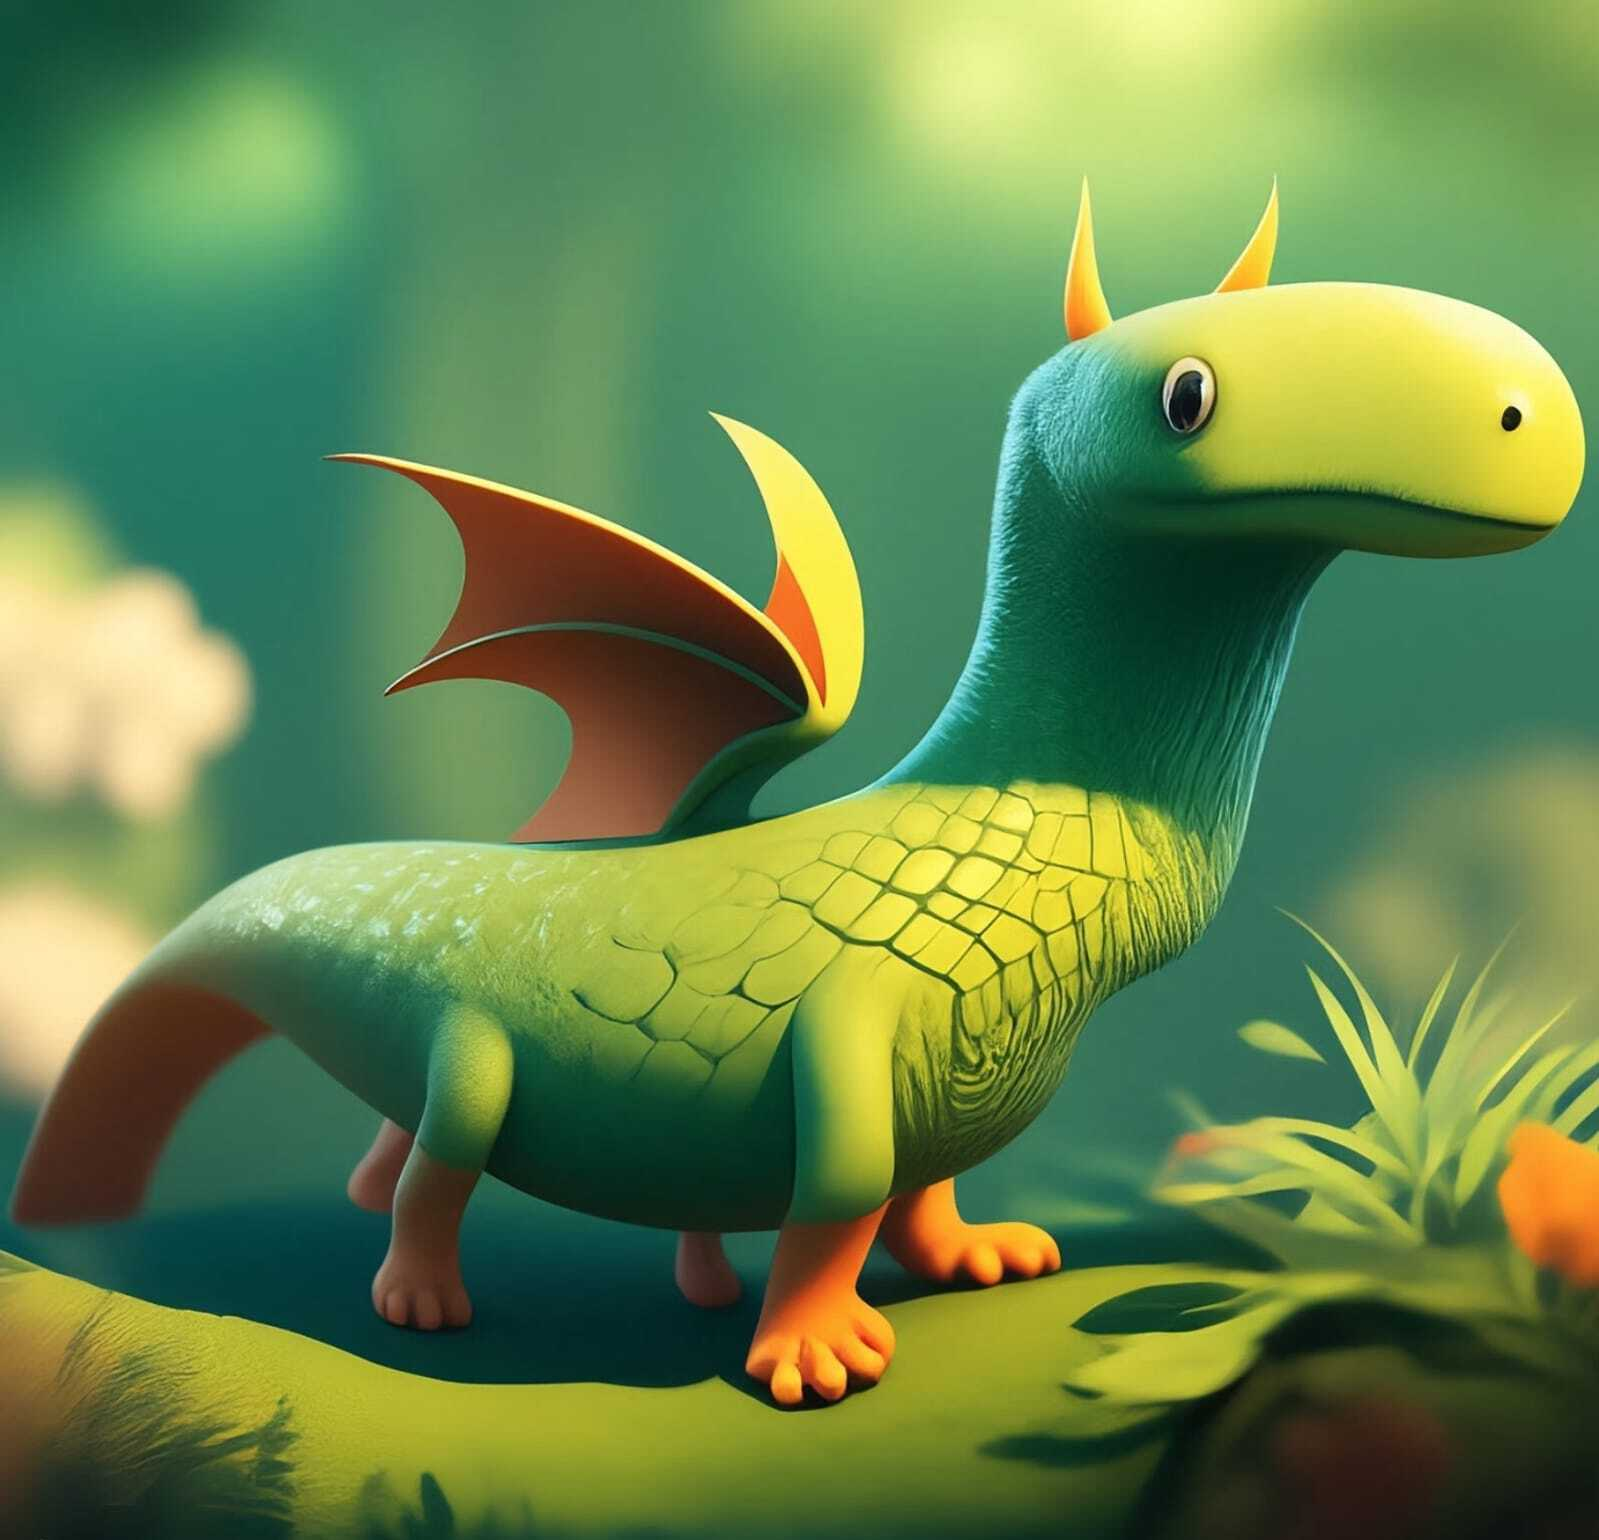
\includegraphics[width=6cm]{cover}
\end{center}
}

% theorem commands
\newtheoremstyle{c_remark}
	{}	% Space above
	{}	% Space below
	{}% Body font
	{}	% Indent amount
	{\bfseries}	% Theorem head font
	{}	% Punctuation after theorem head
	{.5em}	% Space after theorem head
	{\thmname{#1}\thmnumber{ #2}\thmnote{ \normalfont{\text{(#3)}}}}	% head content
\newtheoremstyle{c_definition}
	{3pt}	% Space above
	{3pt}	% Space below
	{}% Body font
	{}	% Indent amount
	{\bfseries}	% Theorem head font
	{}	% Punctuation after theorem head
	{.5em}	% Space after theorem head
	{\thmname{#1}\thmnumber{ #2}\thmnote{ \normalfont{\text{(#3)}}}}	% head content
\newtheoremstyle{c_plain}
	{3pt}	% Space above
	{3pt}	% Space below
	{\itshape}% Body font
	{}	% Indent amount
	{\bfseries}	% Theorem head font
	{}	% Punctuation after theorem head
	{.5em}	% Space after theorem head
	{\thmname{#1}\thmnumber{ #2}\thmnote{ \text{(#3)}}}	% head content

\ifcsname c@english\endcsname
	\theoremstyle{plain}
	\newtheorem{theorem}{Theorem}[section]
	\newtheorem{lemma}[theorem]{Lemma}
	\newtheorem{proposition}[theorem]{Proposition}
	\newtheorem*{proposition*}{Proposition}
	%\newtheorem{corollary}[theorem]{אין חלופה עברית}

	\theoremstyle{definition}
	\newtheorem{definition}[theorem]{Definition}
	\newtheorem*{definition*}{Definition}
	\newtheorem{example}{Example}[section]
	\newtheorem{exercise}{Exercise}[section]

	\theoremstyle{remark}
	\newtheorem*{remark}{Remark}
	\newtheorem*{solution}{Solution}
	\newtheorem{conclusion}[theorem]{Conclusion}
	\newtheorem{notation}[theorem]{Notation}
\else
	\theoremstyle{c_plain}
	\newtheorem{theorem}{משפט}[section]
	\newtheorem{lemma}[theorem]{למה}
	\newtheorem{proposition}[theorem]{טענה}
	\newtheorem*{proposition*}{טענה}
	%\newtheorem{corollary}[theorem]{אין חלופה עברית}

	\theoremstyle{c_definition}
	\newtheorem{definition}[theorem]{הגדרה}
	\newtheorem*{definition*}{הגדרה}
	\newtheorem{example}{דוגמה}[section]
	\newtheorem{exercise}{תרגיל}[section]

	\theoremstyle{c_remark}
	\newtheorem*{remark}{הערה}
	\newtheorem*{solution}{פתרון}
	\newtheorem{conclusion}[theorem]{מסקנה}
	\newtheorem{notation}[theorem]{סימון}
\fi

% Questions related commands
\newcounter{question}
\setcounter{question}{1}
\newcounter{sub_question}
\setcounter{sub_question}{1}

\ifcsname c@english\endcsname
	\newcommand{\question}[1][0]{
		\ifthenelse{#1 = 0}{}{\setcounter{question}{#1}}
		\section{Question \arabic{question}}
		\addtocounter{question}{1}
		\setcounter{sub_question}{1}
	}

	\newcommand{\subquestion}[1][0]{
		\ifthenelse{#1 = 0}{}{\setcounter{sub_question}{#1}}
		\subsection{Part \alph{sub_question}}
		\addtocounter{sub_question}{1}
	}
\else
	\newcommand{\question}[1][0]{
		\ifthenelse{#1 = 0}{}{\setcounter{question}{#1}}
		\section{שאלה \arabic{question}}
		\addtocounter{question}{1}
		\setcounter{sub_question}{1}
	}

	\newcommand{\subquestion}[1][0]{
		\ifthenelse{#1 = 0}{}{\setcounter{sub_question}{#1}}
		\subsection{סעיף \localecounter{letters.gershayim}{sub_question}}
		\addtocounter{sub_question}{1}
	}
\fi

% import lua and start of document
\directlua{common = require ('../common')}

\GetEnv{AUTHOR}

% headers
\author{\AUTHOR}
\date\today

\title{מבנים אלגבריים 1 --- סיכום}
\setcounter{secnumdepth}{2}

\hypersetup{}
\begin{document}
\maketitle
\maketitleprint{}

\tableofcontents

\section{שיעור 1 --- 6.5.2024}
\subsection{מבוא לחבורות}
הקורס עוסק בעיקרו בתורת החבורות, ממנה גם מתחילים. \\*
חבורה (באנגלית Group) היא מבנה מתמטי. \\*
ברעיון חבורה מייצגת סימטריה, אוסף השינויים שאפשר לעשות על אובייקט ללא שינוי שלו, קרי שהוא ישאר שקול לאובייקט במקור. \\*
מה הן הסימטריות שיש לריבוע? אני יכול לסובב ולשקף אותו בלי לשנות את הצורה המתקבלת והיא תהיה שקולה. חשוב להגיד שהפעולות האלה שקולות שכן התוצאה הסופית זהה למקורית. \\*
אפשר לסובב ספציפית אפס, תשעים מאה שמונים ומאתיים שבעים מעלות, נקרא לפעולות האלה A, B, C בהתאמה. \\*
בנוסף אפשר לשקף סביב ציר האמצע, ציר האמצע מלמעלה, ועל האלכסונים, ניתן גם לאלה שמות, נקרא לפעולות אלה בהתאמה $D, E, F, G, H$. \\*
אלה הפעולות הבסיסיות ואי אפשר לעשות פעולה שלא בקבוצה הזאת, אבל אפשר להרכיב את הפעולות האלה והתוצאה הסופית תהיה שקולה לפעולה מהקבוצה. \\*
נגדיר את הפעולות:
\[
	D_4 = \{ A, B, C, D, E, F, G, H \},
	\circ : D_4 \times D_4 \to D_4
\]
נראה כי הרכבת פעולות שקולה לפעולה קיימת:
\[
	E \circ G = C,
	E \circ B = H,
	B \circ F = F
\]
חשוב לשים לב שהפעולה הזאת לא חילופית: $X \circ Y \ne Y \circ X$. \\*
היא כן קיבוצית: $X \circ (Y \circ Z) = (X \circ Y) \circ Z$. \\*
תכונה נוספת היא קיום האיבר הנייטרלי, במקרה הזה $A$. איבר זה לא משפיע על הפעולה הסופית, והרכבה איתו מתבטלת ומשאירה רק את האיבר השני:
\[
	\forall X \in D_4 : A \circ X = X \circ A = X
\]
התכונה האחרונה היא קיום איבר נגדי:
\[
	\forall X \in D_4 \exists Y \in D_4 : X \circ Y = Y \circ X = A
\]

\begin{definition}[חבורה]
	חבורה היא קבוצה $G$ עם $\circ : G \times G \to G$ ואיבר $e \in G$ כך שמתקיימות התכונות הבאות:
	\begin{enumerate}
		\item אסוציאטיביות (חוק הקיבוץ): $\forall x, y, z \in G : (x \circ y) \circ z = x \circ (y \circ z)$.
		\item קיום איבר נייטרלי: לכל $x \in G$ מתקיים $x \circ e = e \circ x = x$.
		\item קיום איבר נגדי: לכל $x \in G$ קיים $y \in G$ כך שמתקיים $x \circ y = y \circ x = e$.
	\end{enumerate}
	חשוב לציין כי זו היא לא הגדרה מיניממלית, ניתן לצמצם אותה, לדוגמה להגדיר שלכל איבר יש הופכי משמאל בלבד (יש להוכיח שקילות).
\end{definition}

\begin{lemma}[קיום איבר נייטרלי יחיד]
	אם $e_1, e_2 \in G$ נייטרליים אז $e_1 = e_2$.
\end{lemma}
\begin{proof}
	$e_1 = e_1 \circ e_2 = e_2$
\end{proof}
דהינו, קיים איבר נייטרלי יחיד.

\subsection{דוגמות}
הקורס מבוסס על הספר ''מבנים אלגבריים'' מאת דורון פודר, אלכס לובוצקי ואהוד דה שליט, אך יש הבדלים, חשוב לשים לב אליהם. ניתן לקרוא שם דוגמות. \\*
דוגמות כלליות לחבורות,
עבור $(\FF, +, \cdot, 0, 1)$ שדה:
\begin{enumerate}
	\item חבורה החיבורית היא $(\FF, +, 0)$
	\item החבורה הכפלית היא $(\FF, \cdot, 1)$
\end{enumerate}
הסימון הכי נפוץ לפעולה של החבורה היא כפל או נקודה או לא בכלל: $xy = x \cdot y$.
\begin{definition}[חבורה קומוטטיבית]
חבורה $G$ תיקרא קומוטטיבית או חילופית או אבלית (על שם המתטיקאי אבל) אם $xy = yx$ לכל $x, y \in G$. \\*
חשוב להבין, למה שסימטריות תהינה חילופיות.
\end{definition}
\begin{example}[לחבורות קומוטטיביות]
	$(\ZZ, +, 0)$ חבורת החיבור מעל השלמים, היא חבורה קומוטטיבית. \\*
	באופן דומה גם $(\ZZ_n, +, 0)$.
\end{example}
\begin{example}[חבורות לא קומוטטיביות]
	נבחין במספר דוגמות לחבורות שאין בהן חילופיות.
	\begin{itemize}
		\item $(D_4, \circ, A)$ אשר מייצג את הריבוע עליו דובר בתחילת ההרצאה
		\item $S_n$ תמורות על $1, \dots, n$ עם הרכבה. \\*
			תמורה היא פעולה שמחליפה שני איברים כפונקציה, לדוגמה $s(1) = 2, s(2) = 1, s(n) = n$. \\*
			$S_n$ הוא מקרה פרטי של תמורות על קבוצה $\{1, \dots, n \}$
		\item $\text{Sym}(X) = \{ f : X \to X \mid f \text{ הופכית, חח''ע ועל} \}$ \\*
			תמורות הן סימטריה של קבוצה, כל תמורה היא העתקה חד־חד ערכית ועל שמשמרת את מבנה הקבוצה.
		\item $GL_n(\FF)$ מטריצות $n \times n$ הפיכות מעל שדה $\FF עם כפל$.
		\item אם $V$ מרחב וקטורי מעל שדה $\FF$ אז \\*
	$GL(V) = \{ f : V \to V \mid f \text{ לינארית וחד חד ערכית} \}$
	\end{itemize}
	נשים לב כי $GL_n(\FF) \cong GL(\FF^n)$, דהינו הם איזומורפיים. זה לא אומר שהם שווים, רק שיש להם בדיוק אותן תכונות. \\*
	גם בקבוצות שתי קבוצות עם אתו גודל הן איזומורפיות אך לא שקולות.
\end{example}

\section{תרגול 1 --- 7.5.2024}
\subsection{חבורות ותתי־חבורות}
\begin{example}
	\begin{align*}
		& (\ZZ, \cdot, 1) & \text{לא חבורה בגלל $0$} \\
		& (M_{n \times n}(\RR), \circ, I_n) & \text{לא חבורה בגלל מטריצות רגולריות ומטריצת האפס לדוגמה} \\
		& (\ZZ_4, +_4, 0) & \text{אכן חבורה} \\
		& (\ZZ_3, +_3, 0) & \text{אכן חבורה} \\
		& (\ZZ_4^*, \cdot, 1) & \text{לא חבורה, $2 \cdot 2 = 0$} \\
		& (\ZZ_3^*, \cdot, 1) & \text{אכן חבורה, מבוסס על מספר ראשוני} \\
	\end{align*}
\end{example}
הערה לא קשורה: הסימון של כוכבית מסמן הסרת כלל האיברים הלא הפיכים מהקבוצה. \\*
כל שלישייה $(\ZZ_p\setminus\{0\}, \cdot_p, 1)$ היא חבורה בתנאי ש־$p$ הוא ראשוני.
\begin{lemma}[בסיסיות של חבורות]
	\begin{align*}
		& e_1 = e_1 e_2 = e_2 & \text{יחידות האיבר הנייטרלי} \\
		& x \in G, y, y_1 = x^{-1} : y = y \cdot e = y x y_1 = e \cdot y_1 = y_1 & \text{יחידות ההופכי}
	\end{align*}
	תהי $G$ חבורה, $g = x_1 \cdot \hdots \cdot x_n$ ביטוי לא תלוי בהצבת סוגריים, טענה זו אפשר להוכיח באינדוקציה. \\*
	לכל $n, m \in \NN$ מתקיים גם ${(x^n)}^m = x^{n\cdot m}$ ואף $x^n \cdot x^m = x^{n + m}$.
\end{lemma}
\begin{definition}[תת־חבורה]
	תהי חבורה $(G, \cdot_G, e_G)$, ותהי $H \subseteq G$ תת־קבוצה, אז $(H, \cdot_G, e_G)$ תיקרא תת־חבורה אם היא מהווה חבורה תקינה. נסמן $H \le G$.
\end{definition}
\begin{example}
	$(2\ZZ, +, 0) \le (\ZZ, +, 0)$ חבורת הזוגיים בחיבור היא תת־חבורה של השלמים. \\*
	$(\diag_n(\RR), \circ, I_n) \le (GL_n(\RR), \circ, I_n)$ חבורת המטריצות האלכסוניות היא תת־חבורה של המטריצות. \\*
	$(GL_n(\QQ), \circ, I_n) \le (GL_n(\RR), \circ, I_n)$ מטריצות הפיכות מעל הרציונליים חלקיות למטריצות הפיכות מעל הממשיים.
\end{example}
\begin{proposition}[מקוצר לתת־חבורה]
	תהי $G$ חבורה ותהי קבוצה $H \subseteq G$ אז $H \le G$ (תת־חבורה של $G$) אם ורק אם:
	\begin{enumerate}
		\item $e_G \in H$, איבר היחידה נמצא ב־$H$
		\item $\forall x \in H : x^{-1} \in H$, לכל איבר גם האיבר ההופכי לו נמצא בקבוצה
		\item $\forall x, y \in H : x \cdot y \in H$, הקבוצה סגורה לכפל האיברים בה
	\end{enumerate}
\end{proposition}
\begin{example}
	\begin{align*}
		& (\NN_0, +, 0) \not\subseteq (\ZZ, +, 0) & 1 \in \NN_0 \land -1 \not\in \NN_0 \\
		& \{0, 2, 4, 6, 8\} \subseteq (\ZZ_{10}, +_{10}, 0) & \text{כלל התנאים מתקיימים} \\
	\end{align*}
\end{example}
\begin{proposition}[תת־חבורה לחבורה סופית]
	אם חבורה היא סופית, אז תנאי 2 איננו הכרחי לתתי־חבורות.
	\begin{proof}
		תהי $G$ חבורה סופית ותהי $H \subseteq G$ אשר מקיימת את סעיפים 1 ו־3 בקריטריון. \\*
		יהי $x \in H$, נבחין כי $\{ x^n \mid n \in \NN \} \subseteq H$ בעקבות סעיף 3 של הקריטריון. \\*
		לכן קיימים שני מספרים $n, m \in \NN$ כך ש־$m < n$ אשר מקיימים $x^n = x^m$. \\*
		כמובן מתקיים $x^n \cdot x^{-m} = e$ ומהסגירות לכפל נובע כי $x^{n - m} \in H$ ומצאנו כי התנאי השני מתקיים.
	\end{proof}
\end{proposition}

\subsection{חבורת התמורות}
תהי $X$ קבוצה, אז $\text{Sym}(X)$ היא קבוצת הפונקציות החד־חד ערכיות ועל מ־$X$ לעצמה. \\*
$(\text{Sym}(X), \circ, Id)$ היא חבורה, מורכבת מכלל התמורות, הרכבת פונקציות ופונקציית הזהות. \\*
אם $X$ היא קבוצה סופית אז $S_n = \text{Sym}(X)$, ובדרך כלל נגדיר $X = [n] = \{1, \hdots, n\}$, וחבורת התמורות תהיה $(S_n, \circ, Id)$.

\begin{definition}[סדר של חבורה]
	סדר של חבורה הוא מספר האיברים בחבורה. \\*
	אילו $G$ אז נגיד שסדר החבורה הוא אינסוף. \\*
	נסמן את הסדר $|G|$. \\*
	אילו $G$ חבורה ו־$x \in G$, הסדר של $x$ הוא $n \in \NN$ המינימלי כך שמתקיים $x^n = e$, נסמנו $|x|$ או $\sigma(x)$.
\end{definition}
\subsubsection{חזרה לתמורות}
נשים לב שמתקיים $|S_n| = n !$. \\* % chktex 40
$\sigma \in S_n$, נכתוב את התמורה כך:
\[
	\begin{pmatrix}
		1 & 2 & \cdots & n \\
		\sigma(1) & \sigma(2) & \cdots & \sigma(n)
	\end{pmatrix}
\]
לדוגמה $\begin{pmatrix}
	1 & 2 & 3 \\
	2 & 1 & 3
\end{pmatrix}$. \\*
אילו $\sigma \in S_n$ ו־$i \in [n]$ נקיים $\sigma(i) = i$ אז $i$ נקרא \textbf{נקודת שבט} של $\sigma$. \\*
בדוגמה שנתנו, $\sigma(3) = 3$ ולכן זוהי נקודת שבט של $\sigma$.

\subsubsection{תתי־חבורות של חבורת התמורות}
דוגמה ראשונה:
\[
	\left\{
		\begin{pmatrix}
			1 & 2 & 3 \\
			1 & 2 & 3
		\end{pmatrix},
		\begin{pmatrix}
			1 & 2 & 3 \\
			2 & 1 & 3
		\end{pmatrix}
	\right\}
	\subseteq S_3
\]
היא תת־חבורה של $S_3$ שכן כללי הקריטריון מתקיימים מבדיקה. \\*
גם $\{ \sigma \in S_n \mid \sigma(1) = 1 \}$ היא תת־חבורה, שכן $\sigma(\tau(1)) = \tau(\sigma(1)) = 1$. \\*
לעומת זאת $\{ \sigma \in S_n \mid \sigma(1) \in \{1, 2, 3\}\}$ איננה חבורה. נראה כי אם $\sigma, \tau$ המקיימות $\sigma(4) = 2, \sigma(2) = 4, \tau(2) = 1, \tau(1) = 2$
וכל השאר נקודות שבט, $\sigma(\tau(1)) = 4$ שלא נמצא בקבוצה על־פי הגדרתה.

\subsubsection{מחזורים}
מחזור הוא רצף של איברים שהתמורה מחזירה כרצף, זאת אומרת שהתמורה עבור האיבר הראשון במחזור תחזיר את השני, השני את השלישי וכן הלאה.
\begin{definition}
	מחזור פשוט $\sigma \in S_n$ יקרא \textbf{$l$־מחזור} אם קיימים $x_1, \hdots, x_l \in [n]$ כך שלכל $0 \le i < l$ מתקיים $\sigma(x_i) = x_{i + 1}$ ו־$\sigma(x_l) = x_0$.
\end{definition}
\begin{proposition}
	כל תמורה היא הרכבה של מספר כלשהו של מחזורים, ההוכחה מסתמכת על היכולת לשרשר את ערכי המחזור משרשראות שאינן נוגעות אחת לשנייה.
\end{proposition}
\begin{example}
	נבחין כי אם
	\[
		\sigma = \begin{pmatrix}
			1 & 2 & 3 & 4 & 5 & 6 & 7 \\
			6 & 2 & 7 & 5 & 1 & 4 & 3
		\end{pmatrix}
	\]
	אז נוכל להרכיב $\sigma = (1 \, 6 \, 4 \, 5)(2)(3 \, 7)$. \\*
	נשים לב למקרה מיוחד, יהי $\sigma \in S_n$ כך ש־$\sigma$ הוא $l$־מחזור, ונגדיר $\sigma = (x_1 \, x_2 \, \hdots \, x_l)$. \\*
	בהינתן $\tau \in S_n$, מתקיים
	\[
		\tau \circ \sigma \circ \tau^{-1} = (\tau(x_1) \, \tau(x_2) \, \hdots \, \tau(x_n))
	\]
	זאת שכן לדוגמה $\sigma(\tau^{-1}(\tau(x_1))) = \sigma(x_1)$ ובהתאם $(\tau \circ \sigma \circ \tau^{-1}) (x_1) = \tau(x_1)$.
\end{example}

\section{שיעור 2 --- 8.5.2024}
\subsection{מבוא לאיזומורפיות}
%אנחנו מקבלים את האחריות על תהליך הלמידה בקורס מבחינת שיעורי בית, דהינו מטלות. בבקשה תפתור לבד כמה שאפשר ואשכרה תחשוב על כל שאלה, כדי ללמוד ממנה. \\*
המטרה שלנו היא להבין מתי שתי חבורות שונות הן שקולות, ולחקור את מושג האיזומורפיות. \\*
נבחן את $\ZZ/2$ ואת $(\{\pm 1\}, \cdot)$ ובשתיהן יש רק שני איברים, אחד נייטרלי ואחד לא, ובשתיהן הפעולות מתנהגות אותו דבר בדיוק.
\[
	1 \leftrightarrow -1,
	1 \leftrightarrow 0
\]
עוד דוגמה היא $(\RR, +)$ ו־$(\RR^{>0}, \cdot)$.
\[
	(\RR, +) \xrightarrow{\exp} (\RR^{>0}, \cdot), \exp(x + y) = \exp(a) \exp(b)
\]
\begin{definition}[הומומורפיזם]
	עבור $G$ ו־$H$ חבורות,
	\textbf{הומומורפיזם} מ־$G$ ל־$H$ היא פונקציה $\varphi : G \to H$ שמקיימת:
	\begin{enumerate}
		\item $\varphi(e_G) = e_H$
		\item $\varphi(x y) = \varphi(x) \varphi(y)$
		\item $\varphi(x^{-1}) = {\varphi(x)}^{-1}$
	\end{enumerate}
\end{definition}
\begin{lemma}[תנאי הכרחי להומומורפיזם]
	$\varphi : G \to H$ היא הומומורפיזם אם ורק אם לכל $x, y \in G$ מתקיים $\varphi(xy) = \varphi(x) \varphi(y)$.
\end{lemma}
\begin{proof}
	נראה ששלושת התכונות מתקיימות:
	\begin{enumerate}
		\item נבחר $x \in G$ ונראה כי $\varphi(x) = \varphi(e_G x) = \varphi(e_G) \varphi(x) \iff e_H = \varphi(e_G)$.
		\item נתון
		\item $\varphi(e_G) = \varphi(x x^{-1}) = \varphi(x) \varphi(x^{-1}) = e_H \implies \varphi(x^{-1}) = \varphi^{-1}(x) e_H$
	\end{enumerate}
	ומצאנו כי שלושת התנאים מתקיימים.
\end{proof}

\begin{definition}[איזומורפיזם]
	איזומורפיזם $G$ ל־$H$ הוא הומומורפיזם חד־חד ערכי ועל ומסומן $\varphi : G \xrightarrow{\sim} H$.
\end{definition}

\begin{lemma}[הופכי לאיזומורפיזם]
	עבור $\varphi : G \xrightarrow{\sim} H$ גם ההופכי הומומורפיזם (ולכן גם איזומורפיזם).
\end{lemma}
\begin{proof}
	נראה כי לכל $x, y \in H$:
	\[
		\varphi^{-1}(xy)
		= \varphi^{-1}(\varphi(\varphi^{-1}(x)) \varphi(\varphi^{-1}(y)))
		= \varphi^{-1}(x) \varphi^{-1}(y)
	\]
	ומצאנו כי התנאי ההכרחי להומומורפיזם מתקיים.
\end{proof}

\begin{conclusion}[תנאי הכרחי לאיזומורפיזם]
	המומורפיזם $\varphi : G \to H$ הוא איזומורפיזם אם ורק אם קיים הומומורפיזם $\psi : H \to G$ כך שמתקיים $\varphi \circ \psi = \psi \circ \varphi = Id_G$.
\end{conclusion}

\begin{definition}[איזומורפיות]
	נגדיר שתי חבורות כ\textbf{איזומורפיות} אם ורק אם קיים איזומורפיזם ביניהן. \\*
	נשים לב שמספר האיזומורפיזמים בין החבורות, גם אם הוא אינסופי, הוא חסר משמעות, ובמקום אנו מסתכל על עצם האיזומורפיות.
\end{definition}
דוגמה לחבורות איזומורפיות הן $(\{\pm 1\}, \cdot) \cong \ZZ/2$ כפי שראינו בהתחלה. \\*
חשוב לשים לב שגם אם יש כמות איברים זהה בין החבורות, הן לא בהכרח תהינה איזומורפיות, לדוגמה
$GL_2(\FF_2)$, חבורת המטריצות ההפיכות מעל שדה עם שני איברים. יש בשורה העליונה 3 אפשרויות, ובשורה השנייה 2 ולכן יש 6 איברים בחבורה הזו.
גם ב־$S_3$ יש בדיוק שישה איברים, אבל $GL_2(\FF_2) \not\cong S_3$. גם החבורה החיבורית $\ZZ/6$ היא חבורה עם שישה איברים. החבורה הראשונה לא קומוטטיבית והשנייה כן, כי כפל מטריצות לא ניתן לשינוי סדר.
\begin{lemma}[הרכבת הומומורפיזמים]
	$\varphi : G \to H$ ו־$\psi : H \to K$ שני הומומורפיזמים, אז גם $\psi \circ \varphi : G \to K$ הוא הומומורפיזם.
\end{lemma}
\begin{proof}
	$\forall x, y \in G : (\psi \circ \varphi) (xy) = \psi(\varphi(xy)) = \psi(\varphi(x) \varphi(y)) = \psi(\varphi(x)) \psi(\varphi(y)) = (\psi \circ \varphi)(x) (\psi \circ \varphi)(y)$
\end{proof}
\begin{conclusion}[הרכבת איזומורפיזמים]
	הרכבה של איזומורפיזמים היא איזומורפיזם.
\end{conclusion}
\begin{definition}[אוטומורפיזם]
	אוטומורפיזם של $G$ הוא איזומורפיזם $G \xrightarrow{\sim} G$. נסמן ב־$Aut(G)$ את קבוצת האוטומורפיזמים של $G$.
\end{definition}
\begin{lemma}[חבורת האוטומורפיזמים]
	$Aut(G)$ היא חבורה ביחס להרכבה.
\end{lemma}
\begin{proof}
	הרכבה היא אסוציאטיבית, העתקת הזהות מוכלת בקבוצה ונייטרלי להרכבה, והוכחנו שלכל אוטומורפיזם $\varphi$ יש הופכי $\varphi^{-1} \in Aut(G)$.
\end{proof}
מהי $Aut(\ZZ)$? לדוגמה $\varphi(n) = n + 1$. פונקציה זו איננה אוטומורפיזם שכן $\varphi(1 + 3) = \varphi(4) = 5, \varphi(1) + \varphi(3) = 6$. \\*
פונקציית הזהות היא אוטומורפיזם, והפונקציה $\varphi(n) = -n$ על־פי בדיקה ישירה של הגדרות. \\*
נבחן את פונקציית הכפל בקבוע, $\varphi(n) = 2n$, נראה כי $\varphi(n + m) = 2(n + m) = 2n + 2m, \varphi(n) + \varphi(m) = 2n + 2m$. הומומורפיזם, אבל לא כל איבר שייך לקבוצה השנייה ולכן לא אוטומורפיזם.
\[
	Aut(\ZZ) = \{Id, -Id\} \cong \ZZ/2
\]
\begin{proposition}[ערך $Aut(Z)$]
	$Aut(\ZZ) = \{Id, -Id\}$.
\end{proposition}
\begin{proof}
	יהי $\varphi : \ZZ \xrightarrow{\sim} \ZZ$, ראשית נראה כי $\varphi(n) = n\varphi(1)$. \\*
	עבור $n = 0$ ברור, עבור $ n > 1$ נראה כי $\varphi(n) = \varphi(1 + \cdots + 1) = \varphi(1) + \cdots + \varphi(1) = n \varphi(1)$. \\*
	עבור $n \le 1$ נשתמש ב־$\varphi(-1) = -1$ ובהתאם $\varphi(-n) = (-n)\varphi(1)$. תתקן אחר כך את הסימנים. \\*
	לכן $\varphi(1) = \pm 1 \implies \varphi = \pm Id$.
\end{proof}
\begin{definition}[מכפלת חבורות]
	אם $G$ ו־$H$ הן חבורות, המכפלה הישרה ל $G$ ו־$H$ או $G \times H$ היא החבורה שמקיימת $G \times H = \{ (x, y) \mid x \in G, y \in H \}$.
	עם הפעולה $(x_1, y_1) \cdot (x_2, y_2) = (x_1 x_2, y_1 y_2)$ והנייטרלי $e = (e_G, e_H) \in G \times H$ \\*
	נראה בהמשך שמתקיים $\ZZ/6 \cong \ZZ_2 \times \ZZ_3$. אבל $\ZZ/4 \not\cong \ZZ/2 \times \ZZ/2$.
\end{definition}
\begin{definition}[תת־חבורה]
	$G$ חבורה, ותהי תת־קבוצה $H \subseteq G$ נקראת תת־חבורה אם
	\begin{enumerate}
		\item $e \in H$
		\item $x, y \in H \implies xy \in H$
		\item $x \in H \implies x^{-1} \in H$
	\end{enumerate}
\end{definition}
נשים לב  כי תת־קבוצה $H \subseteq G$ היא תת־חבורה אם ורק אם $H$ חבורה ביחס לאותה פעולה של $G$. \\*
מסמנים $H \le G$ תת־חבורה. \\*
דוגמות:
\begin{itemize}
	\item $\{ 0^\circ, 90^\circ, 180^\circ, 270^\circ \} \le D_4$
	\item $\{ \sigma \in S_n \mid \sigma(1) = 1 \} \le S_n$
		\subitem{-} תהי $G$ חבורה סופית אז $Aut(G) \le Sym(G) \cong S_n$
	\item $SL_n(\FF) \le GL_n(\FF)$ מטריצות עם דטרמיננטה 1 הן חלקיות למטריצות הפיכות.
	\item $B_n(\FF) \le GL_n(\FF)$ מטריצות משולשיות עליונות עם אלכסון 1 הן חלקיות אף הן להפיכות.
	\item $O_n(\FF) \le GL_n(\FF)$ חבורת המטריצות האורתוגונליות חלקיות לחבורת המטריצות ההפיכות. $O_n(\FF) = \{ A \in GL_n(\FF) \mid I_n = AA^t = A^t A$.
\end{itemize}
\begin{lemma}[חיתוך תת־חבורות]
	לכל קבוצה $S$ ומשפחה $\{ H_\alpha \le G \mid \alpha \in S\}$. של תת־חבורה של $G$ אז $\bigcap_{\alpha \in S} H_\alpha \le G$ תת־חבורה. \\*
	הערה קטנה: משפחה היא קבוצה של קבוצות ככה שאפשר לזהות כל אחת לפי מספר, אפשר להשתמש בלמה גם בקבוצות כרגיל.
\end{lemma}
\begin{proof}
	\begin{itemize}
		\item $e \in H_\alpha$ לכל $\alpha \in S$ ולכן $e \in \bigcap_{\alpha \in S}$.
		\item $x, y \in \bigcap_{\alpha \in S}$ אם ורק אם לכל $\alpha$ מתקיים $x, y \in H_\alpha$ ולכן $xy \in H_\alpha$ ובהתאם $xy \in \bigcap_{\alpha \in S}$.
	\end{itemize}
	ומצאנו כי זוהי חבורה.
\end{proof}
למשל $SO_n = SL_n(\RR) \cap O_n \le GL_n(\RR)$.
\begin{definition}[תת־חבורה נוצרת]
	$G$ חבורה ו־$S \subseteq G$, תת־קבוצה, התת־חבורה הנוצרת על־ידי $S$ מוגדרת להיות:
	\[
		\langle S \rangle = \bigcap_{S \subseteq H \le G} H
	\]
\end{definition}
נשים לב כי על־פי הלמה האחרונה מתקבל כי זוהי אכן תת־חבורה.

\section{שיעור 3 --- 15.5.2024}
\subsection{תת־חבורות}
\begin{definition}[תת־חבורה נוצרת]
	תהי $S \subseteq G$ תת־קבוצה לחבורה, נגדיר
	\[
		\langle S \rangle = \bigcap_{S \subseteq H \le G} H \le G
	\]
\end{definition}
\begin{lemma}[תת־חבורה מינימלית]
	$S \subseteq G$ התת־חבורה המינימלית $\langle S \rangle$ היא התת־חבורה המינימלית של $G$ המכילה את $S$.
\end{lemma}
קצת קשה לעבור על זה, איזה אפיון נוסף יש לדבר הזה?

\begin{proposition}[תת־חבורה נוצרת מפורשת]
	$S \subseteq G$ אז
	\[
		\langle S \rangle = \overline{S} \equiv \{ x_1^{\epsilon_1}x_2^{\epsilon_2} \cdots x_n^{\epsilon_n} \mid x_i \in S, \epsilon_i = \pm 1 \}
	\]
\end{proposition}
\begin{proof}
	\textbf{כיוון ראשון:}
	נניח שעבור תת־חבורה $H$ המכילה של $S$ סגיורת $H$ לכפל והופכי גוררת שהקבוצה $\overline{S}$ הנתונה מוכלת ב־$H$. \\*
	מצד שני נראה שזוהי כבר תת־חבורה.
	\begin{itemize}
		\item $1 \in \overline{S}$ מכפלה ריקה.
		\item $x, y \in \overline{S}$ אז נסמן
			\[
				x = x_1^{\epsilon_1}x_2^{\epsilon_2} \cdots x_n^{\epsilon_n},
				y = y_1^{\epsilon_1}y_2^{\epsilon_2} \cdots y_n^{\epsilon_n},
				xy = x_1^{\epsilon_1}x_2^{\epsilon_2} \cdots x_n^{\epsilon_n} y_1^{\epsilon_1}y_2^{\epsilon_2} \cdots y_n^{\epsilon_n}
			\]
		\item $x \in \overline{S}$ אז
			\[
				x^{-1} = x_1^{-\epsilon_1}x_2^{-\epsilon_2} \cdots x_n^{-\epsilon_n},
			\]
			וידוע כי $(x y)(x^{-1} y^{-1}) = x y x^{-1} y^{-1} = x x^{-1} = 1$
	\end{itemize}
\end{proof}

\begin{definition}[שלמות תת־חבורה יוצרת]
	אם $\langle S \rangle = G$ אומרים ש־$S - e$ יוצרת את $G$.
\end{definition}
\begin{example}
	מתקיים $\langle -1 \rangle = \langle 1 \rangle = \ZZ$. כקונספט כללי $\langle d \rangle = d\ZZ$. \\*
	מה לגבי $\ZZ/n$? מתקיים $\langle 1 \rangle = \ZZ/n$.
\end{example}
\begin{definition}[חבורה ציקלית]
	חבורה $G$ נקראת \textbf{ציקלית} אם היא נוצרת על־ידי איבר אחד, דהינו קיים $x \in G$ כך ש־$\langle x \rangle = G$.
\end{definition}
\begin{proposition}
	כל חבורה ציקלית $G$ מקיימת $G \simeq \ZZ$ או $G \overset{\sim}{=} \ZZ/n$ הוכחה בתרגיל.
\end{proposition}
\begin{example}
	$G = D_4$. \\*
	נגדיר את $\sigma$ להיות סיבוב בתשעים מעלות, ואת $\tau$ להיות היפוך על ציר האיקס. \\*
	אז יש לנו את $\langle \sigma \rangle = \{e, \sigma, \sigma^2, \sigma^3\}$ \\*
	וגם $\langle \tau \rangle = \{e, \tau\}$. \\*
	אנחנו יכולים להכפיל כל שני איברים משתי הקבוצות שסימנו עכשיו.
	\[
		D_4
		= \langle \sigma, \tau \rangle
		= \{e, \sigma, \sigma^2, \sigma^3,
		\tau, \sigma \tau, \sigma^2 \tau, \sigma^3 \tau \}
	\]
	נראה כי לדוגמה $\tau \sigma = \sigma^3 \tau, \sigma^4 = e, \tau^2 = e$. \\*
	ונראה כי $\tau \sigma \tau^{-1} = \sigma^3 = \sigma^{-1}$.
\end{example}
\begin{proposition}[תת־חבורות של Z]
	לכל $H \le \ZZ$ קיים $d \ge 0$ יחיד כך ש־$H = d \ZZ$.
\end{proposition}
\begin{proof}
	אם $H \ne \{0\}$ אז קיים $0 < d \in H$ וניקח את $d$ להיות המינימלי שמקיים את אי־השוויון. \\*
	מצד אחד $\langle d \rangle = d \ZZ \subseteq H$. \\*
	מצד שני, עבור $a \in H$ וידוע $a > 0$ אז נכתוב $a = nd + r$ כאשר $0 \le r < d$ שארית. \\*
	נקבל כי $r = a - nd \in H$. מהמינימליות של $d$ נובע כי $r = 0$ ולכן $a = nd \in d\ZZ$.
\end{proof}
יחידות של זה: תרגיל
נגלה בהמשך שתת־חבורה של חבורה ציקלית היא בעצמה ציקלית.

\begin{definition}[gcb]
	עבור שני מספרים $a, b \in \ZZ$ שלא שניהם $0$ נגדיר $\gcd(a, b) = d$ (Greatest common divisor) מחלק משותף מקסימלי כך שמתקיים:
	$d \mid a, b$ וגם לשלכל $m \mid a, b$ מתקיים גם $m \mid d$.
\end{definition}
\begin{proof}
	$\langle a, b \rangle = d\ZZ$, לאיזשהו $d \ge 0$ יחיד. \\*
	נראה ש־$d = \gcd(a, b)$. \\*
	מצד אחד $a, b \in d \ZZ$ ולכן $d \mid a, b$. \\*
	מצד שני אם $n \mid a, b$ אז $d \in d \ZZ = \{a, b \} \subseteq m \ZZ$. ולכן $m \mid d$ והוא מחלק מקסימלי.
\end{proof}
 \begin{example}
	 עבור $2 \ZZ = \langle 2 \rangle = \langle 6, 10 \rangle$
 \end{example}
 \begin{conclusion}[הלמה של Bézout]
	 לכל $a, b \in \ZZ$ קיימים $n, m \in \ZZ$ עבורם $\gcd(a, b) = na + mb$.
\end{conclusion}

\subsection{מחלקות (Cosets)}
\begin{definition}[מחלקה ימנית ושמאלית]
	תהי $G$ חבורה ו־$H \le G$ ו־$x \in G$. 
	נגדיר את המחלקה השמאלית של $x$ על־ידי
	\[
		x H = \{x h \mid h \in H\}
	\]
	ואת המחלקה הימנית של $x$ בהתאם
	\[
		H x = \{h x \mid h \in H\}
	\]
\end{definition}
\begin{exercise}
	הראו כי המחלקות הימניות והשמאליות הן איזומורפיות, והראו כי זה לא מתקיים עבור מונואידים.
\end{exercise}

\begin{lemma}[שיוך למחלקה]
	$y \in xH \iff yH = xH$
\end{lemma}
\begin{proof}
	\[
		y \in xH
		\iff  y = x h
		\iff x^{-1} y \in H
		\iff y^{-1} x \in H
		\iff x \in yH, y \in xH
		\iff xH = yH
	\]
\end{proof}
\begin{conclusion}
	לכל $x, y \in G$ מתקיים \\*
	$x H = y H$ (אם ורק אם $x^{-1} y \in H$). \\*
	או $xH \cup yH = \emptyset$
\end{conclusion}
\begin{proof}
	אם $z \not\in xH \cup yH$ אז מהלמה הקודמת $yH = ZH = xH$.
\end{proof}

\begin{proposition}[כיסוי זר]
	$G \le H$ התת־קבוצות מהצורה $xH$ עבור $x \in G$ מהוות כיסוי זר של $G$.
\end{proposition}
\begin{proof}
	נשאר לשים לב $x \in xH$ ולכן כיסוי ומהמסקנה זר.
\end{proof}

\begin{proposition}
	לכל $x, y \in G$ יש התאמה חד־חד ועל ערכית של קבוצות $xH \xrightarrow{\sim} yH$. \\*
	בפרט אם $H$ סופית אז לכל המחלקות אותו גודל, $|xH| = |yH|$.
\end{proposition}
\begin{proof}
	נגדיר
	$\varphi : xH \to yH$ על־ידי $\varphi(z) = y x^{-1} z$. \\*
	ונגדיר פונקציה חדשה $\psi : yH \to xH$ על־ידי $\psi(z) = x y^{-1} z$. \\*
	אז מתקיים $\psi = \varphi^{-1}$ ובהתאם נובע כי $\varphi$ איזומורפיזם.
\end{proof}

\begin{definition}[אוסף מחלקות]
	$H \le G$ אז נסמן
	\[
		G / H = \{ xH \mid x \in G \},
		H \backslash G = \{ Hx \mid x \in G \}
	\]
	אוסף המחלקות השמאליות והימניות בהתאמה.
\end{definition}
\begin{theorem}[משפט לאגרנז']
	אם $G$ חבורה סופית, אז לכל $H \le G$ מתקיים $\left. |H| \Big| |G| \right. $.
\end{theorem}
\begin{proof}
	ל־$G$ יש כיסוי זר על־ידי מחלקות שמאליות של $H$ ולכן הגודל של $|G| = |H| \cdot |G / H|$. \\*
	הגודל של $|G / H| = |G| / |H|$.
\end{proof}
\begin{notation}
	$|G / H| = |G : H|$ \textbf{האינדקס} של $H$ ב־$G$.
\end{notation}

\begin{example}
	המחלקות של $3\ZZ \le \ZZ$:
	\[
		3\ZZ + 0 = 3\ZZ + 3, 3\ZZ + 1, 3\ZZ + 2
	\]
	הקבוצה $\ZZ/3\ZZ$ היא השאריות האפשריות בחלוקה לשלוש.
\end{example}

\section{שיעור 4 --- 20.5.2024}
\subsection{סדר}
\begin{definition}[סדר של חבורה]
	$G$ חבורה ו־$x \in G$ מסומן $o(x)$ הוא המספר הקטן ביותר כך ש־$1 \le n \in \NN, x^n = e$. או $\infty$ אם לא קיים $n$ כזה.
\end{definition}
\begin{lemma}[סדר]
	\[
		o(x) = | \langle x\rangle|
	\]
\end{lemma}
\begin{proof}
	נוכיח שאם $o(x)$ סופי אז
	\[
		\langle x \rangle = \{ 1, x, x^2, \hdots, x^{o(x) - 1} \} \tag{1}
	\]
	ואם $o(x) = \infty$ אז
	\[
		\langle x \rangle = \{ 1, x, x^2, \hdots, \} \cup \{ x^{-1}, x^{-2}, \hdots \} \tag{2}
	\]
	הוכחה ל־$(1)$. \\*
	$(1)$ תת־חבורה:
	\begin{itemize}
		\item $x^k \cdot x^m \equiv x^{(m + k) \mod o(x)}$.
		\item ${(x^n)}^{-1} = x^{o(x) - n}$.
	\end{itemize}
	כל ההאיברים שונים כי אם $x^k = x^m$ ל־$0 \le k < k \le o(x)$ אז
	\[
		1 = x^0 = m^{m - k}
	\]
	ונקבל $1 \le m - k < o(x)$ בסתירה למינימליות של $o(x)$. \\*
	הוכחה ל־$(2)$: \\*
	אם $H = \langle x \rangle$. \\*
	סופיות נתונה בקבוצה.
	\[
		\{1, x, x^2, \hdots \} \subseteq H
	\]
	מסופיות קיימים $0 \le k < m$ עבורם
	\[
		x^k = x^m \implies x^{m - k} = 1
	\]
	ולכן ל־$x$ יש סדר סופי, משובך היונים. \\*
	$2$ תרגיל.
\end{proof}
\begin{conclusion}[משפט לגרנז' לחבורה סופית]
	$G$ חבורה סופית, אז לכל $x \in G$ מתקיים
	\[
		o(x) \Big| |G|
	\]
\end{conclusion}
\begin{conclusion}
	אם קיים $x \in G$ עבורו $o(x) = |G|$ אז $G$ ציקלית.
\end{conclusion}

\begin{proposition}[בסיס למשפט השאריות הסיני]
	לכל $a, b \ge 1$ זרים אז $\gcd(a, b) = 1$, מתקיים
	\[
		\ZZ/a \times \ZZ/b \cong \ZZ/ab
	\]
\end{proposition}
\begin{proof}
	נראה שהסדר של $x = (1, 1) \in \ZZ/a \times \ZZ/b$ הוא $ab$ ונסיק מההבחנה. \\*
	ראשית, $x^{ab} = (ab, ab) = (0, 0) = 1$. \\*
	מצד שני, אם $x^n = 1$ אז $(n, n) = (0, 0) \in \ZZ/a \times \ZZ/b$ כלומר
	\[
		0 = n \in \ZZ/a, \qquad 0 = n \in \ZZ/b
	\]
	ולכן $a | n, b | n$, $a, b$ זרים ולכן $ab | n$. \\*
	מכיוון ש־$|\ZZ/a \times \ZZ/b| = |\ZZ/a| \cdot |\ZZ/b| = ab$ \\*
	נובע ש־$\ZZ/a \times \ZZ/b$ ציקלית מגודל $ab$ ולכן איזומורפית ל־$\ZZ/ab$.
\end{proof}

\subsection{פעולות של חבורה על קבוצה}
נתעסק בחבורות לא אבליות ואיך הן מופיעות כסימטריות פעמים רבות.
הסיבה שאנחנו מתעסקים בחבורות היא לראות את הפעולות שלהן על דברים.
\begin{definition}[פעולה]
	פעולה של חבורה $G$ על קבוצה $X$ זו פונקציה $\cdot : G \times X \to X$, $(g, x) \mapsto g \cdot x$ כך שמתקיים:
	\begin{enumerate}
		\item $1 \cdot x = x$ לכל $x \in X$.
		\item $h \cdot (g \cdot x) = (hg) \cdot x$ לכל $x \in X, g, h \in G$.
	\end{enumerate}
	סימון: $G \acts X$. באנגלית Group action.
\end{definition}
\begin{example}[לפעולות]
	מספר פעולות:
	\begin{enumerate}
		\item $S_n$ פועלת על הקבוצה $X = \{1, 2, \hdots, n\}$ על־ידי
			\[
				S_n \times \{1, \hdots n\} \to \{1, \hdots, n\}
			\]
			כאשר $(\sigma, k) \mapsto \sigma(k)$.
		\item $D_n \le S_n$ כפי שהגדרנו בתרגיל. \\*
			$D_n$ פועלת על $\{1, 2, \hdots, n \}$ באותו אופן כמו $S_n$, והיא אינטואיטיבית שקולה לביצוע פעולה סימטרית נתונה על מצב מסוים של הריבוע.
		\item $\RR^n \acts GL_n(\RR)$ על־ידי
			\[
				GL_n(\RR) \times \RR^n \to \RR^n, \qquad (A, v) \mapsto Av
			\]
			קבלת וקטור ומטריצה וכפל הווקטור במטריצה. \\*
			$\RR^n \acts O_n(\RR) \le GL_n(\RR)$ פעולה אורתוגונלית על וקטורים, שקול למעשה ל־$S^{n - 1}$. \\*
			$SO_2(\RR) = O_2(\RR) \cap SL_n(\RR)$. אף היא פעולה על $\RR$. \\*
			\textbf{הערה:} הסימון $O(n) = O_n(\RR)$ הוא קבוצת האורתוגונליים על $\RR$, באופן דומה $SO_n(\RR)$ קבוצת האורתוגונליים עם דטרמיננטה $1$.
		\item דוגמה 0: המקרה הטריוויאלי, כל חבורה $G$ ולכל קבוצה $X$ יש את הפעולה הטריוויאלית של $G$ על $X$ והיא
			\[
				g \cdot x = x, \forall g \in G, x \in X
			\]
	\end{enumerate}
\end{example}

הרציונל מאחורי ההגדרה הזאת הוא שאנחנו יכולים לפרק את החבורות מתוך פעולות שאנחנו כבר מכירים ולחקור את התכונות של הפעולות האלה באופן ריגורזי ושיטתי.
נשים לב לדוגמה ש־$D_4 \acts \{ D_1, D_2 \}$, אנחנו יכולים לחקור את המקרה היחסית טריוויאלי הזה של סימטריה גאומטרית על־ידי הגדרת הפעולה המתאימה.

\begin{definition}[אינבולוציה]
	נבחן את הפעולה של $\ZZ/2$ על $X$. האיבר הנייטרלי לא עושה כלום ולכן קל להגדיר אותו, יש להגדיר פעולה רק עבור איבר לא נייטרלי. \\*
	זה אותו דבר בגדול כמו פונקציה $\tau : X \to X$ שמקיימת $\tau \circ \tau = Id_X$, זאת שכן
	\[
		\ZZ/2 \times X \to X, \qquad g \cdot x \mapsto \begin{cases}
			x, & g = 0 \\
			\tau(x), & g = 1
		\end{cases}
	\]
	לפונקציה כזאת קוראים אינבולוציה, פעולה שריבועה הוא $Id$, באנגלית Involution, וכבר ראינו פונקציות רבות כאלה.
\end{definition}

כדוגמה יש לנו לפחות שלוש פעולות $\ZZ/2$ על $\RR^2$ כאלה
\[
	\tau( \begin{bmatrix} x \\ y \end{bmatrix}) = \begin{bmatrix} -x \\ y \end{bmatrix}, \qquad
	\tau( \begin{bmatrix} x \\ y \end{bmatrix}) = \begin{bmatrix} x \\ -y \end{bmatrix}, \qquad
	\tau( \begin{bmatrix} x \\ y \end{bmatrix}) = \begin{bmatrix} x \\ y \end{bmatrix}
\]

\begin{definition}[הפעולה הרגולרית]
$G$ חבורה, \textbf{הפעולה הרגולרית (השמאלית)} של $G$ על $G$ שנתונה על־ידי
\[
	g \cdot x = gx
\]
פעולה המוגדרת על־ידי הכפל של החבורה. זוהי כמובן פעולה והסימון הוא $G \acts G$.
\end{definition}
האם פעולה ימנית גם עומדת בהגדרת הפעולה? \\*
נבדוק את $G \times G \to G$ המוגדרת על־ידי $(g, x) \mapsto xg$: \\*
נבדוק אסוציאטיביות
\[
	h \cdot (g \cdot x) = h \cdot (xg) = (xg)h, \quad (hg) \cdot x = x (hg), \quad (xg) h \ne x (hg)
\]
ומצאנו כי הביטויים לא שווים ואין שמירה על אסוציאטיביות כחלק מהגדרת הפעולה, ולכן כמובן זוהי לא פעולה. \\*
נשתמש במקום זאת בהופכית ונגדיר $(g, x) \mapsto x g^{-1}$ \\*
פעולה זאת היא אכן פעולה מוגדרת והיא נקראת \textbf{הפעולה הרגולרית הימנית}.

יש עוד פעולה מעניינת של חבורה על עצמה, על־ידי הצמדה
\begin{definition}[הצמדה]
	\[
		G \times G \to G, \quad (g, x) \mapsto x g x^{-1}
	\]
	היא פעולת ההצמדה, נחקור אותה בתרגיל. באנגלית Conjugacy.
	באופן דומה הפעולה היא conjugate.
\end{definition}

בהינתן פעולה של $G \acts X$ נגדיר פונקציה $f : G \to Sym(X) \subseteq End(X)$ על־ידי
\[
	f(g)(x) = g \cdot x
\]
זאת שכן $G \times X \to X$ שקול ל־$G \to \{ X \to X \}$.

\begin{proposition}[הצמדה היא הומומורפיזם]
	$f$ היא הומומורפיזם של חבורות.
\end{proposition}
\begin{proof}
	\[
		f(hg)(x) = (hg) \cdot x = h \cdot (g \cdot x) = f(h)(g \cdot x) = f(h)(f(g)(x)) = (f(h) \cdot f(g))(x)
	\]
\end{proof}

למה $f(g) \in Sym(X)$? \\*
כי $f(g^{-1}) \cdot f(g) = f(g^{-1} g) = f(1) = Id$.
גם $f(g) \cdot f(g^{-1}) = f(g g^{-1}) = f(1) = Id$.

בשיעור הבא נגדיר המון דברים על פעולות על קבוצות, אז צריך להבין את זה ואת הדוגמות באופן מאוד כבד ושלם.

\section{תרגול 3 --- 21.5.2024}
\subsection{שאלות מתרגיל 1}
\subsubsection{שאלה 1}
\[
	End(X) = \{ f : X \to X \}
\]
והיה צריך להוכיח שזה מונואיד. וזה חבורה רק כשהקבוצה היא הקבוצה הריקה או יחידון או משהו כזה. \\*
הסעיף השני הוא שיהא $M$ מונואיד כך שלכל $x \in M$ קיים הופכי משמאל ומראים ש־$M$ חבורה.
\begin{proof}[פתרון]
	יש לי $x \in M$ וצריך להראות שקיים $y \im M$ כך ש־$xy = yx = e$. \\*
	נתון קיום של $y \in M$ כך ש־$yx = e$ ואנחנו רוצים להראות שגם $xy \in M$.
	\[
		xy = e \implies {(xy)}^2 = e = x (yx) y = xy = e
	\]
	ולכן $\exists t \in M: tz = e$ ונקבל $z = tz^2 = tz = e$.
\end{proof}
עכשיו נגיד שיש לנו מונואיד $M$ כך ש־$x \in M$ ול־$x$ יש הופכי מימין והופכי משמאל וצריך להראות שהם שווים.
\begin{proof}[פתרון]
	קיימים $y, z, xz = yx = e$. \\*
	לכן
	\[
		z = ez = (yx) z = y (xz) = y
	\]
\end{proof}
הסעיף האחרון הוא לתת דוגמה לאיבר במונואיד עם הופכי משמאל ולא מימין. \\*
נבחן את $End(\NN)$ ונבחר את $f(x) = x + 1$ ו־$g(x) = \begin{cases}
	1, & x = 1 \\
	n - 1, & n > 1
\end{cases}$

\subsubsection{שאלה 4}
סעיף ב', צריך להראות שזה איזומורפי
\[
	\varphi : (\RR^\times, \cdot) \to \ZZ/2 \times \RR^+
\]
ונאחנו משתמשים בבינאריות של $\ZZ/2$, ואנחנו יודעים שלוגריתם משמר פעולות.
\[
	\varphi(x) = \begin{cases}
		(1, \ln|x|), & x < 0 \\
		(0, \ln|x|), & x > 0
	\end{cases}
\]
ועכשיו לסעיף ג': \\*
צריך למצור פונקציה
\[
	\varphi : GL_2(\ZZ/2) \xrightarrow{\sim} S(\{v_1, v_2, v_3\}), \qquad v_1 = (1, 0), v_2 = (0, 1), v_3 = (1, 1)
\]
\[
	\varphi(T) = \begin{pmatrix}
		v_1 & v_2 & v_3 \\
		T(v_1) & T(v_2) & T(v_3)
	\end{pmatrix}
\]
\[
	\varphi(T) \varphi(S) =
	\begin{pmatrix}
		v_1 & v_2 & v_3 \\
		T(v_1) & T(v_2) & T(v_3)
	\end{pmatrix}
	\begin{pmatrix}
		v_1 & v_2 & v_3 \\
		S(v_1) & S(v_2) & S(v_3)
	\end{pmatrix}
	=
	\begin{pmatrix}
		v_1 & v_2 & v_3 \\
		T(S(v_1)) & T(S(v_2)) & T(S(v_3))
	\end{pmatrix}
\]
וזה מן הסתם עובד די טוב. אז בקיצור זה איזומורפיזם. ועכשיו נתחיל באשכרה תרגול.

\subsection{מחלקות שקילות}
\begin{definition}
	תהא $G$ חבורה, ו־$H \le G$.
	מחלקות השקילות השמאליות של $H$ הן קבוצות מהצורה $g H, g \in G$.
\end{definition}
\begin{lemma}[תכונות מחלקות שקילות]
	תהי $H \le G$ חבורה ותת־חבורה, אז הטענות הבאות מתקיימות:
	\begin{enumerate}
		\item $gH = H \iff g \in H$
		\item אם $H$ סופית אז לכל $g \in G$ מתקיים $|g H| = |H|$.
		\item $\forall g \in G : g H = H g \iff g H g^{-1} \subseteq H$.
		\item ישנה התאמה בין הקבוצות $g H$ ל־$H g$.
	\end{enumerate}
\end{lemma}
\begin{definition}[אינדקס]
	תהי $H \le G$ חבורה ותת־חבורתה. \\*
	נגדיר $[G : H]$ להיות מספר המחלקות השמאליות של $H$.
	אם מספר זה אינסופי אז נגדיר את האינדקס $[G : H] = \infty$.
	מספר זה נקרא אינדקס של $H$ ב־$G$.
\end{definition}
\begin{example}
	נתבונן ב־$D_3$.
	חבורת הסימטריות על משולש שווה צלעות.
	יש לנו שלושה צירי סימטריה, ויש לנו שלושה סיבובים לעשות.
	\[
		D_3 = \{ r, r^2, f, fr, fr^2 \}
	\]
	וזה מן הסתם מקיים $D_3 = \langle r, f \rangle$. \\*
	נגדיר $H_1 = \{e, f_2\}, H_2 = \{e, r, r^2\}$. \\*
	נראה כי מחלקות שקילות הן:
	\[
		r H_1 = \{ r, rf \},
		r^2 H_1 = \{ r^2, r^2f \},
		H_1 = H_1
	\]
	ומהצד השני:
	\[
		H_1 r = \{ r, fr \},
		H_1 r^2 = \{ r^2, f r^2 \}
	\]
	ועבור $H_2$:
	\[
		f H_2 = \{ f, fr, fr^2 \}, etc
	\]
\end{example}
עתה נדבר על סדר.
\subsection{משפט לגרנז'}
\begin{definition}[סדר של איבר]
	תהא $G$ חבורה סופית ו־, לכן $g \in G$ נגדיר את הסדר של $g$, או $|g| = ord(g)$ הוא המינימום של המספרים הטבעיים כך ש־$g^n = e$.
\end{definition}
\begin{theorem}[משפט לגרנז']
	תהא $G$ חבורה סופית ו־$H$ תת־חבורה של $G$. אז
	\[
		[G : H] = \frac{|G|}{|H|}
	\]
	ובפרט $|H| \Big| |G|$.
\end{theorem}
\begin{conclusion}
	תהא $G$ סופית ו$g \in G$ אז $ord(g) \Big| |G|$.
\end{conclusion}
\begin{proof}
	על־ידי התבוננות ב־$H = \langle g \rangle$.
\end{proof}
\begin{lemma}
	$|H| = ord(g)$.
\end{lemma}
\begin{proof}
	נגדיר $\varphi : \ZZ/ord(g) \to H$ על־ידי $\varphi(b) = g^n$. \\*
	נראה כי $\varphi$ חד־חד ערכית ועל. \\*
	יהיו $n, m \in \ZZ/ord(g)$ ונניח כי $\varphi(n) = \varphi(m)$, אזי $g^n = g^m$ ולכן $g^{n - m} = e$ ולכן $n - m = 0$, שאם לא כן יש סתירה למינימליות של $ord(g)$. \\*
	מה החבורה הנוצרת על־ידי $\langle g \rangle = \{ g^n \mid n \in \NN\}$. \\*
	יהא $n \in \ZZ$ נחלק את $n$ עם שארית בסדר של $g$, $n = m \cdot ord(g) + r$ ו־$r \in \ZZ/ord(g)$. לכן $g^n = g^{m \cdot ord(g) + r} = g^r$. \\*
	הראינו כי $|H| = ord(g)$ ולכן הסדר של $ord(g) \Big| |G|$.
\end{proof}
\begin{conclusion}
	תהיה $G$ חבורה סופית.
	\[
		\forall g \in G, g^{|G|} = e
	\]
\end{conclusion}
\begin{proof}
	לפי המסקנה הקודמת
	\[
		g^{|G|} = g^{k \cdot ord(g)} = g^{ord(g)} = e
	\]
\end{proof}
\begin{conclusion}
	יהיה $p$ ראשוני, ו־$G$ חבורה מסדר $p$. אז
	\begin{enumerate}
		\item $G$ ציקלית.
		\item $G$ איזומורפית ל־$\ZZ/p$.
		\item כל החבורות מגודל $p$ איזומורפיות.
	\end{enumerate}
\end{conclusion}
\begin{proof}
	$G$ היא לא חבורה טריוויאלית בגלל $p$ ולכן נוכל להגדיר $g \in G \setminus \{e\}$. \\*
	נשים לב כי $1 < ord(g)$ אך מצד שני $|\langle g \rangle| = ord(g) \big|p$ \\*
	לכן $\langle g \rangle = G, |\langle g \rangle| = p$. \\*
	סעיף ב' בתרגיל 2.
\end{proof}
\begin{theorem}[משפט פרמה הקטן]
	יהיה $p$ ראשוני, ו־$a \in \ZZ$, אם $\gcd(a, p) \equiv 1$ אז $a^{p - 1} \equiv 1 (\mod p)$
\end{theorem}
\begin{proof}
	נתבונן בחבורה הכפלית של $\ZZ/p$, מסומנת $\ZZ^\times_{/p}$ שהוא השדה בלי 0 \\*
	הגודל של $\ZZ^\times_{/p}$ הוא $p - 1$ ולכן לכל $x$ בחבורה הזאת $x^{p - 1} =_{\ZZ/p} 1$. \\*
	כעת נחלק את $a$ ב־$p$ עם שארית, ונקבל $a = np + r$ כאשר $0 < r \le p - 1$, וזה נכון כי הם זרים, דהינו $r \in \ZZ^\times_{/p}$. \\*
	נשים לב כי
	\[
		a^{p - 1} \equiv {(mp + r)}^{p - 1} \implies a^{p - 1} \equiv {(mp + r)}^{p - 1} (\mod p) = \sum_{i = 0}^{n - 1} \binom{p - 1}{i} {(m p)}^{p - 1} \cdot r
		\equiv r^{p - 1} (\mod p)
	\]
	לכן $a^{p - 1} = r^{p - 1} = 1$.
\end{proof}

\subsection{שאלה 4 סעיף א'}
היה צריך למצוא תת־חבורה של $GL_n(\FF)$ שאיזומורפית ל־$S_n$.
\begin{proof}[פתרון]
	אוסף מטריצות הפרמוטציה, $H = \{ A \in M_n(\FF) \mid \text{בכל שורה או עמודה יש איבר בודד שאיננו אפס והוא אחת}\}$. \\*
	המטריצות האלה הן כידוע מטריצות שפשוט מחליפות אגפים בווקטורים ולמעשה זה פשוט תמורה על הווקטורים מסדר $n$. \\*
	$S_n = S([n])$ ולכן נגדיר $\varphi : H \to S_n$ על־ידי $\varphi(A) = \text{התמורה שפועלת על $A$}$.
\end{proof}

\section{שיעור 5 --- 22.5.2024}
נניח שיש לי $G$ חבורה סופית. מלגרז' נובע ש־$H \le G \implies |H| \Big| |G|$.
משפט קושי אומר שאם $p \Big| |G|$ ו־$p$ ראשוני אז קיימת חבורה $H \le G$ כך ש־$|H| = p$. למעשה קיים $x \in G$ עם $o(x) = p$.

\subsection{פעולות על קבוצות}
\begin{notation}
	בהינתן $G \acts X$ נסמן עבור $x, y \in X$ את $x \sim y$ כיחס שמתקיים אם $\exists g \in G : g \cdot x = y$.
\end{notation}
במילים פשוטות, שני איברים בקבוצה הם דומים אם קיים איבר בחבורה שמוביל מאחד מהם לשני. רעיונית מדובר בסימטריה, ולכן הגיוני לשאול אם שני מצבים הם סימטריים ללא קשר למה הפעולה שמשרה את הסימטריה.

\begin{proposition}[יחס שקילות בפעולה על קבוצות]
	$\sim$ הוא יחס שקילות.
\end{proposition}
\begin{proof}
	נבחין כי הגדרת יחס השקילות מתקיימת:
	\begin{itemize}
		\item רפלקסיבי $e \cdot x = x$.
		\item סימטרי: $x \sim y \implies \exists g \in G g \cdot x = y \implies g^{-1} y = x \implies y \sim x$.
		\item טרנזיטיבי: $x \sim y, y \sim z \implies \exists g, h \in G, gx = y, hy = z \implies (hg)x = h (gx) = hy = z \implies x \sim z$
	\end{itemize}
\end{proof}
משמעות הדבר היא שסימטריות הן שקולות. שוב, מדובר ברעיון מאוד הגיוני שכן אם בוחנים את הכול בעיניים של סימטריה. כלל המצבים שסימטריים בזוגות גם סימטריים בכללי.

\begin{definition}[מסלולים]
	בהינתן $G \acts X$, המסלולים של $G$ הם מחלקות השקילות של $\sim$ והמסלול של $x \in X$ הוא
	\[
		O(x) = \{ y \in X \mid y \sim x\} = \{ y \in x \mid \exists g \in G : g \cdot x = y \}
	\]
	\textbf{סימון:} קבוצת המסלולים מסומנת $G \backslash X$.
\end{definition}
\begin{conclusion}
	$X = \bigcup_{O \in G\backslash X} O$, דרך מזעזעת להגיד שהקבוצה המקורית מורכבת מהחלוקה למסלולים שלה.
\end{conclusion}
מהותית אנו מדברים פה על החלוקה של $X$ לפי השקילות, בכל קבוצה יהיו רק איברים ששקולים אחד לשני.
\begin{definition}[נקודת שבת]
	$x \in X$ נקודת שבת של $G$ אם $|O(x)| = 1$.\\*
	כלומר $\forall g \in G : g \cdot x = x$.
\end{definition}
הרעיון הוא שהפעולה על איבר מסוים תמיד מחזירה אותו עצמו, ללא קשר לאיזו סימטריה מהחבורה אנחנו בוחרים.
\begin{definition}[טרנזיטיבית]
	פעולה $G \acts X$ נקראת טרנזיטיבית אם $|G \backslash X| = 1$. \\*
	הפעולה היא טרנזיטיבית אם יש רק קבוצת מסלולים (שהיא חלוקת שקילות) אחת, דהינו שכל איבר בקבוצה סימטרי לכל איבר אחר.
\end{definition}
\begin{conclusion}
	$H \backslash G$ קבוצת המסלולים של $H \acts G$ רגולרית משמאל שקולה ל־$H \backslash G$ קבוצת המחלקות הימניות של $H$ ב־$G$.\\*
	באופן דומה $G / H$ המסלולים של הפעולה $H \acts G$ הרגולרית מימין. \\*
	יש פה התכנסות מאוד אלגנטית גם של הרעיון של מחלקות ימניות ושל השקילויות מבחינת רגולרית משמאל, זו הרי מהותית מגדירה הכפלה של האיברים משמאל, ולכן גם המסלולים מעל התת־חבורה הם המחלקות האלה.
\end{conclusion}
\begin{example}
	נבחין בכמה פעולות שונות וחשובות:
	\begin{enumerate}
		\item $G \acts G$ פעולה רגולרית שמאלית. $\forall x, y \in G, x \sim y \iff g \in G : gx = y$ ותמיד קיים $g$ כזה והוא אף יחיד, $g = yx^{-1}$. לכן יש מסלול אחד והפעולה טרנזיטיבית.
		\item יהי $H \le G$, ונבחן את $H \acts G$, רגולרית משמאל, הפעם $x \sim y \iff \exists h \in H : hx = y \iff yx^{-1} \in H \iff Hx = Hy$ מחלקות ימניות. \\*
			מצאנו הפעם כי יש מסלול בין איברים רק אם הם באותה מחלקה ימנית (על אף שמדובר על רגולרית שמאלית). נראה את המסקנה האחרונה.
		\item $GL_2(\RR) \acts \RR^2$ מטריצות הפיכות פועלות על המרחב $\RR^2$. \\*
			מסלולים: $\{ \{ 0 \}, \RR^2 \setminus \{ 0 \} \}$.\\*
			ביתר פירוט, מטריצות הפיכות משמרות את האי־איפוס, אבל כן נוכל להגיע מכל וקטור לכל וקטור אחר עם המטריצה הנכונה.
			לעומת זאת וקטור אפס ישאר אפס מכל מטריצה שתוכפל בו, ולכן הוא לא סימטרי לאף וקטור אחר בפעולה.
		\item $O_2(\RR) \acts \RR^2$, ידוע כי $O_2(\RR) \le GL_2(\RR)$. הפעם כל וקטור צריך להגיע רק לווקטור מאותו גודל.\\*
			מסלולים: $\{ \{0\}, \{ \{ v \in \RR^2 \mid |v| = a\} \mid a > 0 \} \}$. \\*
			לכל וקטור שנבחר, כל מטריצה בחבורה משמרת את הנורמה שלו, אבל לא את הכיוון, ובהתאם נוכל להסיק שכל שני וקטורים עם אותה נורמה שקולים ונמצאים באותה קבוצה.
		\item $S_n \acts \{1, \dots, n\}$ הפעולה הזו היא טרנזיטיבית. \\*
			זה די טריוויאלי בגדול, נוכל לסדר מחדש את רשימת המספרים בכל דרך על־ידי איזושהי תמורה, ובהתאם כל הסדרים דומים אחד לשני ויש ביניהם מסלול.
		\item כל הדגלים שמחולקים לשלושה פסים בשלושה צבעים, וכל האופציות לבחור את של שלושת הצבעים. יש מן הסתם שמונה דגלים כאלה.\\*
			אפשר להגדיר פעולה $\ZZ/2$ של סיבוב ב־$180^\circ$ ואז אפשר לראות אילו דגלים מתקשרים לאילו דגלים אחרים. יש שישה מסלולים.
	\end{enumerate}
\end{example}

\begin{definition}[מקבע]
	תהינה $G \acts X$, עבור $g \in G$, ונגדיר את ה\textbf{מקבע} להיות $ Fix(g) = \{ x \in X \mid gx = x \}$.\\*
	עוד סימון הוא $X^g$, אבל לא מומלץ להשתמש בו, הוא יחסית מבלבל. \\*
	עבור איבר בחבורה, המקבע הוא כל האיברים בקבוצה שהפעולה לא משנה, הם לא בהכרח נקודות שבת כי אנחנו מדברים פה בהקשר של סימטריה ספציפית.
\end{definition}
\begin{definition}[מייצב]
	יהיו $G \acts X$, אז נגדיר  את המייצב של $x \in X$ להיות $Stab(x) = \{ g \in G \mid g x = x \}$, באנגלית Stabilizer. \\*
	סימון נוסף הוא $G_x$. \\*
	במילים זוהי קבוצת איברי החבורה שלא משנים את $x$, או לחילופין שולחים אותו לעצמו.
\end{definition}
האינטואציה היא שיש איברים שסימטריות מסוימות פשוט לא משפיעות עליהם, ובהתאם המייצב הוא קבוצת הסימטריות הכאלה שנייטרליות לאיבר שבחרנו.

\begin{lemma}[מייצב הוא תת־חבורה]
	$G_x$ תת־חבורה של $G$.
\end{lemma}
\begin{proof}
	נבדוק את הגדרת תת־החבורה:
	\begin{enumerate}
		\item איבר נייטרלי: $e \cdot x = x \implies e \in G_x$.
		\item סגירות לכפל: $\forall g, h \in G, g \cdot x, h \cdot x = x \implies (gh) \cdot x = g \cdot (h \cdot x) = g \cdot x = x \implies gh \in G_x$.
		\item קיום הופכי: $g \in G \implies g \cdot x = x \implies x = g^{-1} \cdot x \implies g^{-1} \in G_x$.
	\end{enumerate}
	מצאנו כי כלל התכונות מתקיימות ולכן $G_x$, המייצב של $x$, הוא תת־חבורה של $G$.
\end{proof}
\begin{definition}[פעולה חופשית]
	$G \acts X$ נקראת חופשית אם $G_x = \{e\}$ לכל $x \in X$. במילים אחרות, הפעולה לעולם לא שולחת איבר לעצמו. \\*
	היא נקראת נאמנה אם $\bigcap_{x \in X} G_x = \{e\}$, החיתוך הזה בכללי גם נקרא גרעין.
\end{definition}
נאמנה זה שם קצת מוזר אבל הוא בגדול מבטיח שאין איבר בחבורה שכל איברי הקבוצה נייטרליים אליו, חוץ מהאיבר הנייטרלי עצמו. \\*
עניין הגרעין הוא די דומה למה שקורה בלינארית גם, איבר שהפעולה איתו לא משפיעה על אף איבר בקבוצה.
\begin{definition}
	נבחן את $G \acts G$ על־ידי הצמדה.
	\[
		O(x) = \{ g x g^{-1} \mid g \in G\}
	\]
	המסלול של $x$ הוא קבוצת האיברים שמקיימים $g x g^{-1} = y$, באופן מאוד דומה למטריצות דומות.
	נקרא למסלול הזה מחלקת צמידות.
\end{definition}
\begin{definition}[מרכז]
	ישנו המרכז של $x$ ב־$G$ והוא $C_G(x) = G_x = \{ g \in G \mid g x g^{-1} = x\} \iff gx = xg$. באנגלית Centrilizer.\\*
	מרכז הוא סוג של מייצב במקרה שבו $X = G$.
\end{definition}
\begin{theorem}[מסלול־מייצב]
	$G \acts X$ ו־$x \in X$. $|O(x)| = [G : G_x]$. וזה נכון גם כשהחבורה לא סופית. $O(x) \xrightarrow{\sim} G/G_x$.\\*
	בפרט אם $G$ סופית אז $|O(x)| = \frac{|G|}{|G_x|}$ וונובע שהגודל של כל מסלול מחלק את גודל החבורה. \\*
	במילים הטענה היא שהמסלול של $x$, שהוא מספר האיברים שאפשר להגיע אליהם ממנו, שווה לאינדקס של המייצב, דהינו מספר מחלקות השקילות השונות שאפשר ליצור בעזרת מחלקות שמאליות עם התת־חבורה שלא מושפעת מ־$x$.
\end{theorem}
\begin{proof}
	נגדיר $f : G/G_x \to O(x)$ ונראה שהיא חד־חד ערכית ועל.\\*
	נבחר $f(gG_x) = g \cdot x$. זה לא בהכרח מוגדר היטב ולכן נבדוק למה זה כן.\\*
	אם יש איבר $g' \in gG_x$ אז $g' = g \cdot h$ כך ש־$h \in G_x$. מתקיים ש־$g' \cdot x = g h x \overset{h \in G_x}{=} g \cdot x$.\\*
	על: לפי הגדרה. \\*
	חד־חד ערכי: נניח ש־$g \cdot x = f(g G_x) = f(g'G_x) = g' \cdot x = {(g')}^{-1} g x = x \implies {(g')}^{-1} g \in G_x \overset{\text{סגירות להופכי}}{\implies} g'G_x = g G_x$.
\end{proof}
\begin{example}
	תהינה חבורה $H \le G$ ותת־חבורתה, יש פעולה ''רגולרית'' של $G$ על $G / H$:
	\[
		g \cdot (x H) = (g \cdot x) H
	\]
\end{example}

\begin{theorem}[משפט קושי]
	יהיו $G$ חבורה סופית ו־$p$ ראשוני כך ש־$p \Big| |G|$. אז קיים $x \in G$ כך ש־$ord(x) = p$.
\end{theorem}
\begin{proof}
	נגדיר פעולה של החבורה $\ZZ_{/p}$ על הקבוצה $X = \{ (g_1, \dots, g_p) \in G^p \mid g_1g_2 \cdots g_p = e\}$. \\*
	הפעולה פועלת על־ידי שיפט ציקלי: $u \in \{0, 1, \dots, p - 1\}$ אז $k \cdot (g_1, \dots, g_p) = (g_{k + 1}, g_{k + 2}, \dots, g_{p \mod p}, g_{1}, \dots, g_k)$.\\*
	אז $k (g_{k + 1}, \dots, g_p) = e$ וגם $(g_{k + 1}, \dots, g_p)(g_1, \dots, g_k) = e$. \\*
	נבחין כי כלל המסלולים בפעולה הם אחד משני סוגים:
	\begin{itemize}
		\item מסלולים בגודל $p$. אם לא כל האיברים זהים, מעגל שלם יקח ככמות האיברים והיא מוגדרת להיות $p$.
		\item מסלולים בגודל $1$. אם כל האיברים זהים אז שיפט יחזיר את האיבר עצמו.
	\end{itemize}
	ממשפט מסלול־מייצב $|O(x)| \Big| p \iff |O(x)| = 1, p$.\\*
	עתה נבחין כי אם ישנו מסלול בגודל $p$ אז הוא כמובן ממלא את טענת ההוכחה ולכן נניח שאין כזה. \\*
	נראה כי מסלול בגודל $1$ הוא מסלול שמקיים $(g_1, \dots, g_p) = (g_2, \dots, g_p, g_1)$ כלומר $x = (g, \dots, g)$, $g^p = e$.\\*
	נשים לב כי נוכל לחלק את הקבוצה המקורית ומתקיים $X = \displaystyle \bigcup_{O \in \ZZ_{/p} \backslash X} O$, ובהתאם מהאיחוד הזר נקבל גם $|X| = \displaystyle \sum_{O \in \ZZ_{/p} \backslash X} |O|$. \\*
	אם $(e, \dots, e)$ היה נקודת השבת היחידה אז $\displaystyle \sum_{O \in \ZZ_{/p} \backslash X} |O| \equiv 1 (\mod p)$, שכן כל מסלול כולל $p$ חילופים ונקודת השבת היחידה הייתה תורמת $1$ בלבד. \\*
	לכן מצד אחד $p \Big| |G|^{p - 1}$ ומצד שני $|G|^{p - 1} \cong 1 (\mod p)$ ולכן קיים $x \ne e$ עם $x^n = e$.
\end{proof}
\begin{remark}
	ההוכחה מוויקיפדיה הרבה יותר ברורה.
\end{remark}

\section{שיעור 6 --- 27.5.2024}
\subsection{מקבעים של פעולות}
ניזכר בהגדרת המקבע, $X^g = \{ x \in X \mid gx = x \}$, דהינו האיברים ב־$X$ שלא משתנים על־ידי הסימטריה $g$.

לדגומה עבור החבורה $D_4$ ו־$X = \{1, 2, 3, 4\}$ אוסף קודקודי ריבוע נבחן את $g$ סיבוב על האלכסון: $g = (1\ 3)$ ואת $h = (1\ 2)(3\ 4)$ שיקוף על האמצע.
אז כמובן המקבע של $g$ ב־$X$ הוא $X^g = \{1, 3\}$ אוסף הקודקודים שלא מושפעים מהסימטריה $g$.
באופן דומה $X^h = \emptyset$, דהינו הסמיטריה $h$ תמיד משנה את כל הקודקודים ובהתאם המקבע הוא ריק.

\begin{lemma}[הלמה של ברנסייד]
	תהיה חבורה סופית $G$ ופעולה $G \acts X$ כאשר $X$ סופית גם היא.
	יהי $g \in G$ ונסמן $Fix(g) = X^g = \{ x \in X \mid gx = x\} \subseteq X$. \\*
	אז מספר המסלולים (מסומן גם $X/G$) הוא
	\[
		|X/G| = \frac{1}{|G|} \sum_{g \in G} |Fix(g)|
	\]
	דהינו ממוצע כמות האיברים שנשארים במקום היא ככמות המסלולים השונים.
\end{lemma}
\begin{proof}
	תהי חבורה סופית $G$. עבור $X$ סופית ופעולה $G \acts X$ נגדיר
	\[
		E(X) = \frac{1}{|G|} \sum_{g \in G} |X^g|
	\]
	נוכיח כי $E(x) = |X/G|$.

	נשים לב שאם $X, Y$ קבוצות זרות עם פעולה של $G$, אז נובע מהזרות ומהגדרת המסלולים של הקבוצות כי
	\[
		(X \sqcup Y)/G = X/G \sqcup Y/G
		\implies
		|(X \sqcup Y)/G| = |X/G| + |Y/G|
	\]
	עוד נראה כי	$\forall g \in G : {(X \sqcup Y)}^g = X^g \sqcup Y^g$
	ולכן גם $|{(X \sqcup Y)}^g| = |X^g| + |Y^g|$,
	ונוכל להסיק ש־$|E(X \sqcup Y)| = E(X) + E(Y)$. \\*
	נסיק כי אילו הלמה נכונה עבור $X, Y$ זרים, אז היא מתקיימת גם עבור איחודם $X \sqcup Y$.

	תהי $X$ קבוצה כלשהי, נוכל לכתוב גם
	\[
		X = \bigsqcup_{O \in G\backslash X} O
	\]
	במילים ש־$X$ היא איחוד זר של קבוצות המסלולים השונות שמוגדרות על־ידי הפעולה $G \acts X$. \\*
	על־כן מהטענה שהוכחנו זה עתה מספיק להוכיח את הטענה כאשר ל־$X$ יש מסלול יחיד $x = O$, ובמקרה הכללי נוכל לאחד איחוד זר של מסלולים. \\*
	נניח מעתה כל $X \ne \emptyset$ עם מסלול יחיד (פעולה טרנזיטיבית).
	במקרה הזה צריך להוכיח
	\[
		\frac{1}{|G|} \sum_{g \in G} |X^g| = E(X) = 1
	\]
	נגדיר עבור $x \in X, g \in G$ את $s(g, x)$ על־ידי
	\[
		s(g, x) = \begin{cases}
			1, & gx = x \\
			0, & gx \ne x
		\end{cases}
	\]
	דהינו $s$ מחזירה $1$ אם $g$ מקבעת את $x$. ואנו יודעים כי $X^g = \{ g \in G \mid gx = x \} = \{ g \in G \mid s(g, x) = 1 \}$.
	לכן נוכל להסיק שמתקיים
	\[
		|X^g| = \sum_{x \in G} s(g, x)
	\]
	ועתה נציב ונקבל כי
	\[
		\sum_{g \in G} |X^g|
		= \sum_{g \in G} \sum_{x \in X} s(g, x)
		= \sum_{x \in X} \sum_{g \in G}  s(g, x)
		\overset{(1)}{=} \sum_{x \in X} |G_x|
		\overset{(2)}{=} |X| \cdot |G_x| = |G|
	\]
	$(1)$ נובע ישירות מההגדרה של מייצב $G_x = \{ g \in G \mid g x = x\}$. \\*
	$(2)$ ממשפט מסלול־מייצב נקבל כי $|G| = |G_x| \cdot |O(x)|$ אבל ידוע שהפעולה טרנזיטיבית ולכן $\forall x \in X: O(x) = X$, לכן $|G| = |X| \cdot |G_x|$. \\*
	קיבלנו כי $|E(X)| = 1$ ולכן נוכל להסיק כי הטענה מתקיימת תמיד.
\end{proof}
\begin{example}
	בתזכורת הראינו כי עבור $D_4$ ו־$X = \{1, 2, 3, 4\}$ מתקיים $|X^g| = 2, |X^h| = 0$.
	נחשב את כלל המקבעים ונקבל על־פי הלמה:
	\[
		\frac{1}{8} (4 + 2 + 2 + 0 + 0 + 0 + 0 + 0) = 1 = |D_4 \backslash X|
	\]
	דהינו $D_4$ טרנזיטיבית לפי הלמה, שכן יש לה רק מסלול אחד.
\end{example}
דוגמה נוספת היא בחירת $G$ סופית ופעולה שלה על עצמה עם הצמדה. \\*
לכן $g(h) = ghg^{-1}$ ונשים לב כי המקבע הוא $C(g) = G^g = \{ h \in G \mid ghg^{-1} = h\}$. \\*
כמות מחלקות הצמידות --- היא מספר המסלולים על־פי הצמדה --- ניתנת לחישוב על־ידי
\[
	\frac{1}{|G|} \sum_{g \in G} |C(g)|
\]
\begin{definition}[מרכז חבורה]
	נגדיר את ה\textbf{מרכז} של חבורה $G$, המסומן $Z(G)$, להיות קבוצת האיברים שנייטרליים לסדר ההכפלה בהם:
	\[
		Z(G) = \{ h \in G \mid \forall g \in G : g h = h g\}
	\]
	לחילופין הגדרה שקולה היא קבוצת האיברים שצמודים לעצמם בלבד. \\*
	נגדיר גם $C_x$ מחלקת הצמידות של $x$, דהינו
	\[
		C_x = \{ g \in G \mid g x g^{-1} = x \}
	\]
\end{definition}
\begin{proposition}[מרכז הוא תת־חבורה]
	תהי $G$ חבורה, אז $Z(G) \subseteq G$ היא תת־חבורה.
\end{proposition}
\begin{proof}
	נראה כי תכונות החבורה חלות על $Z(G)$:
	\begin{enumerate}
		\item איבר נייטרלי: $\forall g \in G: eg = ge \implies e \in Z(G)$
		\item סגירות לכפל: $\forall a, b \in G : \forall g \in G, a b g = a g b = g a b \implies ab \in Z(G)$.
		\item סגירות להופכי: $n \in Z(G) : ng = gn \implies \forall g \in G n^{-1} g = g h^{-1}$
	\end{enumerate}
	לכן $Z(G)$ חבורה וחלקית ל־$G$ ולכן נובע $Z(G) \le G$.
\end{proof}

\begin{lemma}[חיתוך מרכזים]
	תהי $G$ חבורה, ניזכר כי המרכז של $x \in G$ מוגדר על־ידי
	\[
		C_G(x) = C(x) = \{ g \in G \mid g x g^{-1} = g \}
	\]
	ומתקיים
	\[
		Z(G) = \bigcap_{x \in G} C(x)
	\]
\end{lemma}
\begin{proof}
	נובע ישירות מההגדרות
\end{proof}
לכן נשים לב שחיתוך המרכזים הוא המרכז של החבורה, והיא תת־חבורה אבלית.

\begin{notation}[מחלקות צמידות]
	תהי חבורה $G$, אז נסמן את אוסף מחלקות הצמידות שלה:
	\[
		cong(G) := \{ X \subseteq G \mid \forall x, y \in X \exists g \in G : x = g y g^{-1} \}
	\]
\end{notation}
נשים לב שמרכז עבור צמידות מסומן באופן מיוחד, וגם כאן זהו סימון מיוחד עבור $G \backslash G$ עם פעולת ההצמדה. \\*
כל איבר ב־$cong(G)$ הוא קבוצה שכלל האיברים בה צמודים זה לזה.
נשתמש בהגדרת המרכז ונכתוב גם
\[
	cong(G) = \{ X \subseteq G \mid \forall x, y \in X : y \in C(x) \}
\]
ונסמן $[g] \in cong(G)$ איבר כלשהו מייצג מכל מחלקת צמידות. \\*
נסמן גם $C_h$ מחלקת הצמידות של $h$ ומתקיים
\[
	C_h = \{ g \in G \mid \exists k \in G : k h k^{-1} = g \}
\]

\begin{proposition}[נוסחת המחלקות]
	תהי חבורה סופית $G$, אז מתקיים
	\[
		|G| = |Z(G)| + \sum_{[h] \in cong(G), h \notin Z(G)} \frac{|G|}{|G_h|}
	\]
\end{proposition}
\begin{proof}
	תחילה נבחין כי נוכל לפרק את $G$:
	\[
		G = \bigsqcup_{[h] \in cong(G)} C_h
	\]
	ונבחין כי לכל $h \in G$ מתקיים
	\[
		h \in Z(G)
		\iff
		|C_h| = 1
		\iff
		\forall g \in G : g h g^{-1} = h
	\]
	אז נוכל לראות כי
	\[
		G = Z(G) \sqcup \bigsqcup_{[h] \in cong(G), h \notin Z(G)} C_h
	\]
	ומכאן נסיק
	\[
		|G|
		= |Z(G)| + \sum_{[h] \in cong(G), h \notin Z(G)} |C_h|
		\overset{\text{מסלול־מייצב}}{=} |Z(G)| + \sum_{[h] \in cong(G), h \notin Z(G)} \frac{|G|}{|G_h| (= |C_G(h))|}
	\]
\end{proof}

\section{תרגול 4 --- 28.5.2024}
\subsection{צביעות}
\begin{definition}[צביעה]
	תהי קבוצה $X$ ותהי צביעה עם $m$ צבעים, אז אז \textbf{צביעה} של $X$ עם $m$ היא פונקציה $f : x \to [m]$.
\end{definition}
הרעיון פה הוא שאנחנו יכולים לקחת את הקבוצה ולסווג לכל איבר בה צבע (מספר) ומן הסתם יש לנו ${[m]}^{|X|}$ צביעות רעיוניות כאלה.
\begin{proposition}[צביעה מעל פעולה]
	תהי קבוצה $X$ ו־$G \acts X$ חבורה ופעולה המסומנת על־ידי $\ldotp$, ויהי ${[m]}^X$ אוסף הצביעות ב־$m$ של $X$. \\*
	אז הפונקציה $\ldotp : G \times {[m]}^X \to {[m]}^X$ המוגדרת על־ידי
	\[
		\forall g \in G, f \in {[m]}^X, \forall x \in X : g \ldotp f(x) = f(g^{-1} \ldotp x)
	\]
	היא פעולה של $G$ על ${[m]}^X$.
\end{proposition}
\begin{proof}
	אנו צריכים לבדוק ששתי התכונות של פעולה של החבורה על הקבוצה מתקיימות.
	\begin{itemize}
		\item נייטרליות האיבר הנייטרלי: $\forall f \in {[m]}^X, x \in X : e \ldotp f(x) = f(e^{-1} x) = f(x)$.
		\item סגירות לכפל: $\forall f \in {[m]}^X, x \in X : g \ldotp (h \ldotp f)(x) = (h \ldotp f)(g^{-1} \ldotp x) = f(h^{-1} g^{-1} \ldotp x) = (gh) \ldotp f(x)$
	\end{itemize}
	ומצאנו כי התנאים לפעולה מתקיימים ומתקיים $G \acts {[m]}^X$.
\end{proof}
מה שבעצם עשינו פה הוא להרחיב פעולה של $G$ על $X$ להשרות פעולה מעל אוסף הצביעות השונות שלו, ועשינו את זה על־ידי שימוש בכפל בהופכי.
מאוד חשוב לשים לב שאנחנו מקבלים את הצביעה כפונקציה של אוסף האיברים ב־$X$ לאוסף הצבעים, אבל זה עדיין איבר בקבוצת הצביעות.

\begin{definition}[שימור צביעה]
	נגדיר שצביעה $f \in {[m]}^X$ נשמרת על־ידי $g \in G$ אם $f \in Fix(g)$, דהינו ש־$g \cdot f = f$.
\end{definition}

\subsection{טטרההדרון}
נבחן עתה את הטטרההדרון (ארבעון) שמרכזו הוא $0 \in \RR^3$ ושקודקודיו מסומנים על־ידי $v_0, \dots, v_3$ ונגדיר אותו מעתה להיות $\Delta^3$.
ונגדיר את חבורת הסימטריה $\Sym(\Delta^3)$ להיות אוסף האיזומטריות הלינאריות שמשמרות את הטטרההדרון:
\[
	\Sym(\Delta^3) = \left\{ T \in GL_3(\RR) \middle| |\det T| = 1, T\Delta^3 = \Delta^3\right\}
\]
ונגדיר גם את חבורת הסימטריות האיזומטריות שנוצרות על־ידי פעולות נוקשות:
\[
	\Sym_+(\Delta^3) = \left\{ T \in \Sym(\Delta^3) \middle| \det T = 1 \right\}
\]

נשים לב כי כל $T \in \Sym(\Delta^3)$ היא למעשה תמורה בין קודקודי הטטרההדרון. יותר מזה גם נשים לב כי אם שתי העתקות סימטריות משנות את הקודקודים באופן זהה אז הן מתנהגות באופן זהה. \\*
נגדיר אם כן את התורה $\sigma_T$ כתמורה שמזיזה את הקודקודים על־פי $T \in \Sym(\Delta^3)$.

\begin{proposition}[פעולת סימטריות על הקודקודים]
	הפעולה $\cdot : \Sym(\Delta^3) \times \{v_0, \dots, v_3\} \to \{v_0, \dots, v_3\}$ הנתונה על־ידי $T \cdot v_i = T(v_i)$ היא פעולה על הקבוצה $\{v_0, \dots, v_3\}$.
\end{proposition}
\begin{proof}
	בתרגיל
\end{proof}
\begin{conclusion}[איזומורפיות הסימטריות]
	הפונקציה $\varphi : \Sym(\Delta^3) \to S(\{v_0, \dots, v_3\})$ המוגדרת על־ידי $\varphi(T) = \sigma^T$ היא איזומורפיזם.
\end{conclusion}
\begin{proof}
	מספיק להוכיח ש־$\varphi$ היא הומומורפיזם ושכל מחזור מהצורה $(v_i, v_j)$ הוא בתמונת $\varphi$.
	העובדה שהיא הומומורפיזם נובעת מיידית מהיותה פעולה על הקבוצה.
	יהיו $i \ne j$ המתארים קודקודים, אז ישנו מישור העובר בין שני הקודקודים האחרים ודרך $\frac{v_i + v_j}{2}$.
	השיקוף סביב מרחב זה שולח את $v_i$ ל־$v_j$ והפוך, בלי להשפיע על שאר הקודקודים.
	לכן $(v_i, v_j) \in \varphi(\Sym(\Delta^3))$. נראה כי $\varphi(\Sym(\Delta^3))$ היא תת־חבורה של $S(\{v_0, \dots, v_3\})$ ולכן היא מכילה קבוצה יוצרת, ומכאן נקבל
	$\varphi(\Sym(\Delta^3)) = S(\{v_0, \dots, v_3\})$, מהטענות הקודמות נקבל גם חד־חד ערכיות.
\end{proof}
מעתה נתייחס באופן שקול ל־$T \in \Sym(\Delta^3)$ ו־$\sigma_T$.
\begin{conclusion}[טרנזיטיביות הפעולה]
	הפעולה של $\Sym(\Delta^3)$ על הקודקודים היא טרנזיטיבית.
\end{conclusion}
\begin{proof}
	נסיק מכך שכל $(v_i, v_j) \in \Sym(\Delta^3)$ שהמסלול של הגעה מכל קודקוד לכל קודקוד הוא יחיד, ולכן ככלל יש מסלול יחיד בפעולה.
\end{proof}

נבחן עתה את הפעולה של $\Sym(\Delta^3)$ על ${[m]}^X$ כאשר $X = \{v_0, \dots, v_3\}$ כפי שהגדרנו בחלק הקודם.

\begin{proposition}[מקבעי הסימטריות]
	יהי $T \in \Sym(\Delta^3)$, אז נוכיח כי $|Fix(T)|$ תלוי בסוג המחזור של $T$ בלבד.
\end{proposition}
\begin{proof}
	נכתוב את כלל סוגי המחזורים ב־$\Sym(\Delta^3)$ על־פי אורכם:
	\begin{align*}
		& 1\ 1\ 1\ 1 \\
		& 2\ 1\ 1 \\
		& 2\ 2 \\
		& 3\ 1 \\
		& 4
	\end{align*}
	מספר התמורות מכל סוג ב־$S_4$ הן $1, 6, 3, 8, 6$ בהתאמה. עתה נחשב את הצביעות המשתמרות על כל מקרה. \\*
	עבור $1\ 1\ 1\ 1$ ישנה רק תמורת הזהות, ובהתאם היא משמרת את הצבע של כל קודקוד, ולכן $|Fix(e)| = m^4$. \\*
	עתה נבחן מחזור בגודל $2$, דהינו $\sigma = (i, j)$. התמורה הזו תשמר את הצביעה של קודקודים אם ורק אם $v_i, v_j$ הם מאותו הצבע.
	לכן לשני הקודקודים $v_i, v_j$ יכולות להיות $m$ צביעות שונות כך שהתמורה תשמר את הצביעה, כאשר שאר הקודקודים בלתי תלויים, ולכן במקרה זה ישנן $m^3$ צביעות משתמרות. \\*
	באופן דומה יש $m^2$ צביעות משתמרות עבור שרשור שני מחזורים מגודל $2$. \\*
	כאשר בוחנים מחזורים בגודל $3$ אז יכולה להיות רק צביעה אחת לשלושת הקודקודים כך שהצביעה תשתמר, ולקודקוד הנותר הצבע חופשי, ונקבל $m^2$. \\*
	עבור תמורות שהן מחזור בודד מגודל $4$ אז על כלל הקודקודים להיות באותו צבע, ונקבל כמובן את מספר הצבעים עצמו $m$.
\end{proof}

נשתמש בלמה של ברנסייד כדי לחשב את מספר המסלולים של סימטריות על קודקודים על צביעות שונות של הקודקודים.
\[
	|\Sym(\Delta^3) \backslash {[m]}^X| = \frac{1}{|\Sym(\Delta^3)|} \sum_{T \in \Sym(\Delta^3)} |Fix(T)| = \frac{1m^4 + 6m^3 + 11m^2 + 6m}{24}
\]
\begin{conclusion}[מסלולים מעל צביעה]
	בעוד הפעולה של הסימטריות על $X$ היא טרנזיטיבית, הפעולה מעל הצביעות היא עצמה לא כזו בהכרח, דהינו הטרנזיטיביות של פעולה לא מעידה על טרנזיטיביות הצביעה מעליה.
\end{conclusion}
\begin{proposition}[כמות הצביעות בסימטריות חיוביות]
	נבחן את הפעולה של $\Sym_+(\Delta^3)$ על הצביעות של הקודקודים ונחשב את כמות המסלולים השונים בה.
\end{proposition}
\begin{proof}[פתרון]
	נובע ממשפט לגרנז'. סיבובים ללא היפוך יכולים להיות מורכבים רק מסיבוב סביב אחת הפאות, ולכן רק ממחזורים מהצורה $(i\ j\ k)$. \\*
	יש כמובן $8$ סיבובים אפשריים כאלה (סביב כל פאה יש שניים).
	לכן יש בחבורה $\Sym_+(\delta^3)$ לפחות 9 איברים יחד עם הנייטרלי, וממשפט לגרנז' נובע כי $\Sym_+(\delta^3) \Big| 24$ ולכן $\Sym_+(\delta^3) \in \{12, 24\}$. \\*
	אבל אנו יודעים כי $|\Sym_+(\delta^3)| < |\Sym(\delta^3)|$ שכן ישנן העתקות שהופכות את הצורה, ולכן נקבל $|\Sym_+(\delta^3)| = 12$. \\*
	נחפש אם כן את שלוש התמורות החסרות. נשים לב כי תמורות מהצורה $(i\ j)(l\ l)$ מוכלות גם הן ב־$\Sym_+(\delta^3)$ שכן הן הופכות את סימן הדטרמיננטה פעמיים.
	לכן נוכל לבחור את התמורה בין שלושה זוגות כפולים של קודקודים ונקבל את שלוש התמורות החסרות.
\end{proof}
\begin{definition}[מספר המסלולים בסימטריות סיבוביות]
	נשתמש בלמה של ברנסייד ונקבל כי מספר המסלולים של $\Sym_+(\delta^3)$ על ${[m]}^X$ היא
	\[
		|\Sym_+(\Delta^3) \backslash {[m]}^X| = \frac{1}{|\Sym_+(\Delta^3)|} \sum_{T \in \Sym_+(\Delta^3)} |Fix(T)| = \frac{1m^4 + 11m^2}{12}
	\]
\end{definition}
\begin{remark}[צביעה של פאות]
	נשים לב כי ישנן ארבע פאות ולכן נוכל לקשר כל פאה לקודקוד ונקבל כי מספר הצביעות של פאות שקול למספר הצביעות של הקודקודים.
\end{remark}

\section{שיעור 7 --- 29.5.2024}
\subsection{חבורות p}
\subsubsection{תזכורת: מרכז של חבורה}
המרכז של חבורה $Z(G)$ הוא תת־חבורה נורמלית של איברים שמתחלפים עם כלל האיברים בחבורה המקורית.
\[
	Z(G) = \{ g \in G \mid \forall h \in, g h = hg \}
\]

\begin{definition}[חבורת p]
	תהי חבורה סופית $G$, אז נקרא ל־$G$ חבורת $p$ אם קיים $p$ ראשוני ו־$n \in \NN$ כך שמתקיים $|G| = p^n$.
\end{definition}
\begin{proposition}[מרכז של חבורת p]
	אם $G$ חבורת $p$ ו־$|G| \ne 1$ ($G$ לא טריוויאלית) אז $|Z(G)| > 1$.
\end{proposition}
\begin{proof}
	למעשה נוכיח ש־$p \Big| |Z(G)|$ ולכן $|Z(G)| \ge p$. \\*
	נשתמש בנוסחת המחלקות
	\[
		|G| = |Z(G)| + \sum_{[h] \in cong(G), n \notin Z(G)} \frac{|G|}{|C_G(h)|}
	\]
	ידוע כבר כי $|G|$ מתחלק ב־$p$ ומספיק לבדוק את הסכום ולקבל את החלוקה. \\*
	כמובן ש־$|G|$ מחולק על־ידי $p$, ולכן גם חלוקתו בגודל מרכז מחולק ב־$p$ או ב־$1$. \\*
	אם $|C(h)| = |G|$ אז $C(h) = G$ ולכן $h \in Z(G)$. ולכן נניח ש־$|C(h)| < |G|$ בלי להגביל את כלליות ההוכחה ונקבל כי $p \Big| \frac{|G|}{|C(h)}$ וקיבלנו כי הסכום מחולק על־ידי $p$.
\end{proof}
\begin{example}
	עבור $S_3$, נקבל $|S_3| = 6$, והמרכז כולל רק את האיבר הטריוויאלי ולכן $|Z(S_n) = 1|$,
	מחלקות הצמידות בתמורות הן תמורות שקולות מחזור ולכן ישנן שלוש מחלקות צמידות, מתוכן שתיים לא במרכז.
	אז נקבל
	\[
		6 = 1 + \frac{6}{3} + \frac{6}{2}
	\]
\end{example}

\subsection{הומומורפיזמים}
ניזכר בהגדרת ההומומורפיזם.
תהינה $G, H$ חבורות אז הומומורפיזם $\varphi : G \to H$ היא העתקה שמקיימת
\[
	\varphi(g_1 g_2) = \varphi(g_1) \varphi(g_2)
\]
ומכאן נובע גם $\varphi(e_G) = e_H$ וגם $\varphi(g^{-1}) = \varphi^{-1}(g)$.
\begin{definition}
	אם $\varphi$ חד־חד ערכית אז נאמר שהיא \textbf{מונומורפיזם}. \\*
	אם היא על היא תיקרא \textbf{אפימורפיזם}. \\*
	אם היא חד־חד ערכית ועל אז היא תיקרא \textbf{איזומורפיזם}.
\end{definition}
\begin{definition}[גרעין]
	יהי $\varphi$ הומומורפיזם $\varphi : G \to H$.
	ה\textbf{גרעין} של $\varphi$ ושמסומן $\ker(\varphi)$ מוגדר להיות
	\[
		\ker(\varphi) = \{ g \in G \mid \varphi(g) = e_H \}
	\]
	כלל האיברים שההעתקה שולחת לאיבר הנייטרלי.
\end{definition}

\begin{definition}[תמונה]
	יהי $\varphi : G \to H$ המומורפיזם, ה\textbf{תמונה} של $\varphi$ המסומנת $\im(\varphi)$ מוגדרת על־ידי
	\[
		\im(\varphi) = \{ h \in H \mid \exists y \in G : \varphi(y) = h \}
	\]
	בדומה לתמונה של פונקציות.
\end{definition}

\begin{proposition}[גרעין ותמונה הם תת־חבורות]
	אם $\varphi : G \to H$ הומומורפיזם אז:
	\begin{enumerate}
		\item $\im(\varphi)$ תת־חבורה של $H$.
		\item $\ker(\varphi)$ תת־חבורה של $G$.
	\end{enumerate}
\end{proposition}
\begin{proof}
	נתחיל בטענה הראשונה, על־פי הגדרת תת־חבורה:
	\begin{enumerate}
		\item איבר נייטרלי: $e_h = \varphi(e_G) \implies e_H \in \im(\varphi)$
		\item סגירות לכפל: $h_1, h_2 \in \im(\varphi) \implies \exists g_1, g_2 : \varphi(g_1) = h_1, \varphi(g_2) = h_2$
		\item סגירות להופכי: $h \in \im(G) \implies \exists g \in \varphi(G) = h \implies \varphi(g) = h^{-1} \implies h^{-1} \in \im(\varphi)$
	\end{enumerate}
	ונוכיח את הטענה השנייה באופן דומה:
	\begin{enumerate}
		\item איבר נייטרלי: $e_G \in \ker(\varphi)$ נובע מ־$\varphi(e_G) = e_H$
		\item סגירות לכפל: $ g_1, g_2 \in \ker(\varphi) \implies \varphi(g_1) = e_H, \varphi(g_2) = e_H \implies \varphi(g_1g_2) = e_H e_H \implies g_1g_2 \in \ker(\varphi)$.
		\item סגירות להופכי: $g \in \ker(\varphi) \implies\ \varphi(g) = e_H \implies \varphi(g^{-1}) = \varphi^{-1}(g) = e_H$
	\end{enumerate}
\end{proof}

\begin{proposition}[תנאי מספיק לאפימורפיזם ומונומורפיזם]
	אם $\varphi$ הומומורפיזם אז:
	\begin{enumerate}
		\item $\im(\varphi) = H$ אם $\varphi$ על (אפימורפיזם).
		\item $\ker(\varphi) = \{e\}$ אם ורק אם $\varphi$ חד־חד ערכית (מונומורפיזם).
	\end{enumerate}
\end{proposition}
\begin{proof}
	טענה 1 היא טריוויאלית ונובעת מההגדרה, נוכיח את הטענה השנייה. \\*
	אם $\varphi$ חד־חד ערכית אז הטענה ברורה. \\*
	נניח כעת כי $\ker(\varphi)$ הוא טריוויאלי ונוכיח כי $\varphi$ חד־חד ערכית. \\*
	נניח בשלילה כי $\exists g_1, g_2 \in G : g_1 \ne g_2, \varphi(g_1) = \varphi(g_2)$. \\*
	נסתכל על $g_2 g_1^{-1} \ne e_G$
	אבל $\varphi(g_2g_1^{-1}) = \varphi(g_2) \varphi(g_1^{-1}) = \varphi(g_2)\varphi^{-1}(g_1) = e_H$.
\end{proof}

נראה עתה מספר דוגמות להומומורפיזמים:
\begin{example}[דטרמיננטה]
	נשים לב כי הדטרמיננטה המוגדרת על־ידי $\det : GL_n(\RR) \to \RR^\times$ היא הומומורפיזם, שכן $|AB| = |A| \cdot |B|$. \\*
	נראה גם כי $\im(|\cdot|) = \RR^\times$ וגם $\ker(| \cdot|) = SL_n(\RR)$.
\end{example}
\begin{example}[מטריצה שקולה למרוכביבם]
	יהי הומומורפיזם $\varphi : C^\times \to GL_2(\RR)$ המוגדר על־ידי 
	\[
		a + bi \mapsto
		\begin{pmatrix}
			a & b \\
			-b & a
		\end{pmatrix}
	\]
	נוכיח כי זהו הומומורפיזם:
	\[
		\varphi(a + ib)\varphi(c + id) = 
		\begin{pmatrix}
			a & b \\
			-b & a
		\end{pmatrix}
		\begin{pmatrix}
			c & d \\
			-d & c
		\end{pmatrix}
		=
		\begin{pmatrix}
			ac - bd & ad + bc \\
			-ad + bc & ac - bd
		\end{pmatrix}
		= \varphi(ac - bd + i(ad + bc))
		= \varphi((a + ib)(c + id))
	\]
	זוהי למעשה העתקה איזומורפית למרוכבים המשמרת כפל מרוכבים.
\end{example}
\begin{example}[העתקות לינאריות]
	כל העתקה לינארית $T : \RR^d \to \RR^m$ היא לינארית ולכן הומומורפיזם.
\end{example}
\begin{example}[בלוקי ז'ורדן]
	ההעתקה $\varphi : \RR \to GL_2(\RR)$ המוגדרת על־ידי
	\[
		a \mapsto \begin{pmatrix}
			1 & a \\
			0 & 1
		\end{pmatrix}
	\]
	היא הומומורפיזם, נוכיח:
	\[
		\varphi(a)\varphi(b)
		=
		\begin{pmatrix}
			1 & a \\
			0 & 1
		\end{pmatrix}
		\begin{pmatrix}
			1 & b \\
			0 & 1
		\end{pmatrix}
		=
		\begin{pmatrix}
			1 & a + b \\
			0 & 1
		\end{pmatrix}
		= \varphi(a + b)
	\]
	נשים לב כי העתקה זו מגדירה עבור כל מספר את בלוק הז'ורדן המתאים אליו, דהינו בלוק ז'ורדן משמר את תכונתו בכפל.
\end{example}
\begin{example}[מטריצה בתמורה]
	נגדיר את ההעתקה $\varphi : S_n \to GL_n(\RR)$ על־ידי
	\[
		\tau \mapsto P_\tau,
		\qquad
		{(P_\tau)}_{ij} = \delta_{i\ \tau(j)}
	\]
	כאשר $\delta_{ij}$ מוגדרת על־ידי
	\[
		(\delta_{ij}) = \begin{cases}
			1, & i = j \\
			0, & i \ne j \\
		\end{cases}
	\]
	זוהי למעשה פונקציה המקשרת תמורה למטריצה הפיכה, על־ידי שינוי סדר השורות להיות על־פי התמורה. נוכיח כי זהו הומומורפיזם:
	\[
		\varphi(\tau)\varphi(\sigma)
		= P_\tau P_\sigma
		= \sum_{k = 1}^{n} {(P_\tau)}_{ik} {(P_\sigma)}_{kj}
		= \delta_{i\ \tau(\sigma(j))}
	\]
	ולכן $P_\tau P_\sigma = P_{\tau \circ \sigma}$ וקיבלנו כי ההעתקה היא הומומורפיזם. \\*
	נוכל לראות כי זהו גם איזומורפיזם, דהינו יש יצוג יחיד לכל תמורה כמטריצה בצורה הנתונה, והפוך.
\end{example}
\begin{example}[צמצום להומומורפיזם]
	אם $\varphi : G \to H$ הומומורפיזם, אז עבור $\im(\varphi) \subseteq H' \subseteq H$ היא תת־חבורה ומתקיים
	\[
		\varphi' : G \to H',
		\qquad
		\varphi'(g) = \varphi(g)
	\]
\end{example}
\begin{example}[שרשור הומומורפיזמים]
	אם $\varphi : G \to H$ וגם $\phi : H \to K$ שני הומומורפיזמים, אז גם $\phi \circ \varphi : G \to K$ הומומורפיזם. \\*
	נוכיח:
	\[
		\phi \circ \varphi(g_1 g_2) = \phi(\varphi(g_1 g_2)) = \phi(\varphi(g_1) \varphi(g_2)) = (\phi \circ \varphi)(g_1) (\phi \circ \varphi)(g_2)
	\]
\end{example}
\begin{example}[סימן של תמורה]
	נבחן את שרשור ההומומורפיזמים:
	\[
		S_n \xrightarrow{P} GL_n(\RR) \xrightarrow{\det} \RR^\times
	\]
	תמונת השרשור היא $\{ -1, 1 \}$ בלבד, נשתמש בהומומורפיזם זה כדי להגדיר סימן לתמורות. \\*
	לתמורות עם סימן חיובי נקרא תמורות זוגיות ולשליליות נקרא אי־זוגיות. \\*
	נגדיר את ההעתקה:
	\[
		sign : S_n \to \{1, -1\} \cong \RR_{/2}
	\]
	ואף נגדיר את תת־חבורת התמורות החיוביות
	\[
		A_n := \ker(sign)
	\]
	אוסף התמורות הזוגיות. \\*
	כך לדוגמה $|A_3| = 3 = |\{e, (1\ 2\ 3), (3\ 2\ 1)\}|$.
\end{example}
\begin{example}[פעולה על חבורה]
	תהי קבוצה $X$ ותהי פעולה $G \acts X$. הפעולה ניתנת להגדרה על־ידי ההעתקה $\varphi : G \to \Sym(X)$, \\*
	שכן $\varphi(g_1 g_2) = \varphi(g_1) \varphi(g_2)$.
	לכן פעולות על קבוצות שקולות להומומורפיזמים מחבורות לסימטריות של $X$.
	נוכיח:
	\begin{proof}
		נגדיר
		\[
			\varphi(g) \in \Sym(X),
			\qquad
			\varphi(g) = fx
		\]
		נבחן את $\varphi(g_1g_2)$ על־ידי הצבה:
		\[
			\varphi(g_1g_2)(x)
			= (g_1 g_2)(x)
			= g_2(g_1(x))
			= \varphi(g)(g_2(x))
			= \varphi(g_1)(\varphi(g_2)(x))
			= (\varphi(g_1) \circ \varphi(g_2))(x)
		\]
	\end{proof}
	זאת למעשה טענה חזקה במיוחד, שכן היא קושרת כל פעולה על חבורה להומומורפיזם בין חבורה לסימטריות של קבוצה ומאפשרת לנו להסיק עוד מסקנות על הפעולה.
\end{example}
\begin{example}[שיכון]
	יהי חבורה ותת־חבורה שלה $H \le G$. \\*
	אז אפשר לבנות את העתקת השיכון ונקבל $\varphi(h \in H) = h \in G$ ונקבל $\im(\varphi) = H$, דהינו כל תת־חבורה יכולה להוות תמונה להומומורפיזם כלשהו.
\end{example}
\begin{proposition}[צמוד לגרעין]
	יהי $\varphi : G \to H$ הומומורפיזם. \\*
	לכל $g \in G$ מתקיים
	\[
		g \ker(\varphi) g^{-1} = \ker(\varphi)
	\]
\end{proposition}
\begin{proof}
	יהי $h \in \ker(\varphi)$ ו־$g \in G$ אז
	\[
		\varphi(g h g^{-1}) = \varphi(g) \varphi(h) \varphi(g^{-1}) = \varphi(g) e_H \varphi^{-1}(g) = e_H
	\]
	וקיבלנו כי השוויון מתקיים.
\end{proof}

\begin{definition}[תת־חבורה נורמלית]
$N \le G$ תת־חבורה של חבורה $G$ נקראת \textbf{נורמלית} אם לכל $g \in G$ מתקיים $g N g^{-1} = N$. \\*
נסמן $N \trianglelefteq G$. \\*
נבחין כי מההגדרה נובע כי כל איבר ב־$N$ הוא חילופי לשאר איברי $G$. \\*
נשים לב כי מצאנו שלכל $\varphi : G \to H$ הומומורפיזם נובע מיידית ש־$\ker(\varphi) \trianglelefteq G$.
\end{definition}

\begin{theorem}[משפט האיזומורפיזם הראשון]
	יהי $\varphi : G \to H$ הומומורפיזם, אז $\im(\varphi) \xrightarrow{\sim} G/\ker{\varphi}$. \\*
	דהינו התמונה של הומומורפיזם והמחלקות השמאליות של הגרעין הן איזומורפיות.
\end{theorem}
\begin{proof}
	נסמן $N = \ker(\varphi)$ אז
	\[
		g N \mapsto \varphi(g) \varphi(N) = \varphi(g) \in \im(g)
	\]
	נוכל לבחור נציג לכל מחלקה שכן:
	\[
		\forall g_1, g_2 \in G : g_1 N = g_2 N \iff g_1 g_2^{-1} \in N \iff \varphi(g g_2^{-1}) = e_h \iff \varphi(g_1) = \varphi(g_2)
	\]
	ומצאנו כי זהו הומומורפיזם. קל לראות כי הוא אף הפיך, ולכן גם איזומורפיזם.
\end{proof}
\begin{theorem}[משפט ההתאמה]
	תהי $G$ חבורה ו־$N \trianglelefteq G$ תת־חבורה נורמלית שלה. \\*
	יש התאמה חד־חד ערכית ועל בין תת־חבורות של $G/N$ לבין תת־חבורות של $G$ המכילות את $N$. \\*
	דהינו קיימת פונקציה חד־חד ערכיתו על $\varphi : \{ H \mid N \le H \le G \} \to \{ K \mid K \le G/N \}$. \\*
	ההתאמה נוצרת על־ידי $\pi : G \to G/N$ הומומורפיזם המתאים לפעולת חלוקה לאגפים. \\*
	התאמה זו שומרת על יחסי הכלה, נורמליות, אינדקסים.
\end{theorem}

\section{שיעור 8 --- 3.6.2024}
\subsection{הומומורפיזמים}
\begin{proposition}[תנאי התמונה לאיזומורפיזם]
	העתקה $f : G \to H$ היא חד־חד ערכית אם ורק אם $G \xrightarrow{\sim} \im(f)$.
\end{proposition}
\begin{example}[דוגמות להומומורפיזמים]
	$D_n \hookrightarrow S_n$ על־פי הגדרה. \\*
	גם $P \cdot S_n \hookrightarrow GL_n(\FF)$ מטריצות הפרמוטציה היא שיכון ואף אחד מאוד חשוב. \\*
	ראינו כי $P : S_n \hookrightarrow GL_n(\FF) \xrightarrow{\det} \RR^\times$ שמייצג סימן עבור תמורות. \\*
	ראינו גם את $\CC^\times \hookrightarrow GL_2(\RR)$ על־ידי $a + bi \mapsto \begin{pmatrix} a & -b \\ b & a \end{pmatrix}$.
\end{example}
ניזכר כי מצאנו קשר בין פעולה לבין הומומורפיזם וננסחו כלמה.
\begin{lemma}[הומומורפיזם ופעולה]
	הומומורפיזם $G \xrightarrow{f} \Sym(X)$ היא זהה לפעולה $G \acts X$  כך שמתקיים
	\[
		\forall g \in G, \pi_g \in \Sym(X) : \pi_g(x) = g \cdot x, \pi_g \circ \pi_h = \pi_{gh}
	\]
	ונסיק $f(g) = \pi_g$ הומומורפיזם. \\*
	עוד נבחין כי $\ker(f) = \{ g \in G \mid \pi_g = Id_X \}$
	ונסיק כי $g \in \ker(G) \iff gx = x \forall x \in X$
	ולכן $\ker(f) = \bigcap_{x \in X} G_x$.
\end{lemma}
\begin{theorem}{משפט קיילי}
	לכל חבורה $G$ קיימת קבוצה $X$ ושיכון $G \hookrightarrow \Sym(X)$. \\*
	אם $|G| = n$ אז יש שיכון $G \hookrightarrow S_n$.
\end{theorem}
\begin{proof}
	$G$ פועלת רגולרית (משמאל) על $G$.
	כלומר $\forall x \in G : G_x = \{e\}$ שכן $gx = x \iff g = e$. \\*
	בפרט אם $f : G \to \Sym(G)$ ההומומורפיזם המתאים אז $\ker(f) = \cap_{x \in G} G_x = \{ e \}$
	וקיבלנו כי $f$ חד־חד ערכית.
\end{proof}
\begin{example}
	נקבל כי $D_n \hookrightarrow S_{2n}$, עוד נקבל מהמשפט שאפשר ליצור את השיכון $S_n \hookrightarrow S_{n!}$.
	זה לא הכי עוזר לנו אבל זה כן אפשרי, אנו רואים כי המשפט מבטיח שיכון אבל הוא עלול להיות די חסר תועלת ומהיכרות עם החבורה נוכל לבנות שיכון מוצלח יותר.
\end{example}
\begin{notation}
	העתקה חד־חד ערכית מסומנת $\hookrightarrow$,
	העתקה על מסומנת $\twoheadrightarrow$.
\end{notation}
\begin{proposition}[תנאי לתת־חבורה נורמלית]
	התנאים הבאים הם שקולים ואם אחד מהם מתקיים אז $N$ תת־חבורה נורמלית.
	\begin{enumerate}
		\item $\forall g \in G : g N g^{-1} \subseteq N$.
		\item $\forall g \in G : g g N g^{-1} = N$.
		\item $\forall g \in G : g N = N g$.
	\end{enumerate}
	ההוכחה בתרגיל.
\end{proposition}
\begin{conclusion}
	לא קיים הומומורפיזם $f : S_3 \to H$ כך שמתקיים $\ker(f) = \{ Id, (1\ 2) \}$.
\end{conclusion}
\begin{proof}
	נבחין כי $\{ Id, (1\ 2)\}$ היא לא תת־חבורה נורמלית של $S_3$ כי $(1\ 3)(1\ 2)(3\ 1) = (1)(2\ 3)$.
\end{proof}
דהינו לא כל תת־חבורה יכולה לשמש כגרעין, נשאל את עצמנו האם כל תת־חבורה נורמלית היא גרעין של הומומורפיזם כלשהו, על שאלה זו נענה עתה.

\begin{proposition}[תמונת תת־חבורה נורמלית]
	כאשר $f : G \to H$ הומומורפיזם ו־$N = \ker(f)$ אז $f^{-1}(f(x)) = x N$, התמונה ההפוכה של תמונת $x$ היא המחלקה $x N$. \\*
	יתרה מכך הפונקציה $\im(f) \to G/N$ המוגדרת על־ידי $h \mapsto f^{-1}(h)$ היא חד־חד ערכית ועל.
\end{proposition}
\begin{proof}
	תחילה נבחין כי מתקיים
	\[
		{f(x)}^{-1} f(y) = x^{-1} y \in N \iff xN = yN
	\]
	נראה כי ההעתקה היא על:
	\[
		f^{-1}(f(x)) = xN
	\]
	נראה כי ההעתקה היא גם חד־חד ערכית,
	עבור $f(x), f(y) \in \im(f)$ מתקיים
	\[
		f^{-1}(f(x)) = f^{-1}(f(y)) = yN
		\iff
		x^{-1} y \in N
		\iff
		f(x^{-1} y) = e
	\]
\end{proof}

\subsection{חבורת המנה}
תהינה $N \triangleleft G$ ונגדיר $G/N$ מבנה של חבורה.

\begin{proposition}[מכפלת מחלקות]
	$N$ נורמלית אם ורק אם $\forall x, y \in G : (xN) \cdot (yN) = (xy)N$.
\end{proposition}
\begin{proof}
	$(x N)(y N) = x (Ny) N \overset{\text{נורמליות}}{=} x (yN) N = (xy)(NN) = (xy)N$
\end{proof}

\begin{proposition}[חבורת כפל מחלקות]
	$G/N$ עם הכפל של מחלקות היא חבורה עם האיבר הנייטרלי $eN$.
\end{proposition}
\begin{proof}
	נבדוק את התנאים לחבורה:
	\begin{enumerate}
		\item איבר נייטרלי: $\forall x \in N: (eN)(xN) = xN = (xN)(eN)$.
		\item אסוציאטיביות: $((xN)(yN))(zN) = ((xy)z)N = (xyz)N = (xN)(yN)(zN)$.
		\item סגירות להופכי: $(xN)(x^{-1}N) = (xx^{-1})N = eN$.
	\end{enumerate}
\end{proof}
\begin{proposition}
	תהי הפונקציה $\pi : G \to G/N$ המוגדרת על־ידי $x \mapsto x N$. \\*
	הפונקציה $\pi$ היא הומומורפיזם כך שגם $\ker(\pi) = N$.
\end{proposition}
\begin{proof}
	$\pi(x) \cdot \pi(y) = (xN)(yN) = (xy)N = \pi(xy)$. \\*
	עוד נבחין כי $x N = \pi(x) = N \iff x \in N$.
\end{proof}
\begin{example}
	נבחין בחבורות המנה הבאות:
	\begin{enumerate}
		\item עבור החבורה $\ZZ$. זוהי חבורה אבלית ולכן כל תת־חבורה שלה היא נורמלית ומתקיים $n \ZZ \triangleleft \ZZ$. \\*
			בהתאם $\ZZ/n \cong \ZZ / n \ZZ = \{ n \ZZ, 1 + n \ZZ, \dots, (n - 1) + n \ZZ \}$. \\*
			ונראה גם $(a + n \ZZ) + (b + n \ZZ) = ((a + b) + n \ZZ) \equiv (a + b \mod n) + n \ZZ$.
		\item ראינו בתרגול כי $GL_n(\FF) / SL_n(\FF) \cong \FF^\times, A \cdot SL_n(\FF) \mapsto \det(A)$. \\*
			ואנחנו רואים כי $\det : GL_n(\FF) \twoheadrightarrow \FF^\times$ וגם כי $SL_n(\FF) = \ker(\det)$.
	\end{enumerate}
\end{example}

\section{תרגול 5 --- 4.6.2024}
\subsection{תת־חבורות נורמליות}
\begin{example}
	תהי $H \subseteq GL_n(\FF)$ חבורת הייזנברג, המוגדרת על־ידי
	\[
		H = \left\{
			\begin{pmatrix}
				1 & a & c \\
				0 & 1 & b \\
				0 & 0 & 1
			\end{pmatrix}
			\middle|
			a, b, c \in \FF
		\right\}
	\]
	נבחין כי זו אכן חבורה שכן מטריצות מולשיות סגורות לפעולת הכפל ומכילות הופכי. \\*
	נגדיר גם
	\[
		Z = \left\{
			\begin{pmatrix}
				1 & 0 & c \\
				0 & 1 & 0 \\
				0 & 0 & 1
			\end{pmatrix}
			\middle|
			c \in \FF
		\right\}
	\]
	נבחין כי $Z \trianglelefteq H$ ואף מתקיים $H/Z \cong \FF^2$.
\end{example}
\begin{lemma}
	תזכורת: אם $|G| = p$ אז $G$ היא ציקלית.
\end{lemma}
\begin{lemma}
	אם $|G| = p^2$ כאשר $p$ ראשוני, אז $G$ אבלית.
\end{lemma}
\begin{proof}
	ידוע כי $Z(G)$ לא טריוואלית, ולפי משפט לגרנז' מתקיים $|Z(G)| \Big| |G|$ אז נקבל כי $|Z(G)| \in \{ p, p^2 \}$. \\*
	נקבל כי $G/Z(G)$ היא מגודל $1$ או מגודל $p$. לכן נקבל כי החלוקה הזו היא ציקלית ואז נובע כי היא אבלית.
\end{proof}
נבחין כי לא בהכרח כל $G$ ציקלית היא מגודל $p^2$, לדוגמה ${(\ZZ_{/p})}^2$ היא לא ציקלית כלל שכן לא כל האיברים הם מסדר $p$ ועל־כן אי־אפשר ליצור את החבורה מאיבר בודד. נשים לב לכן גם ש־${(\ZZ/p)}^2 \not\cong \ZZ_{/p^2}$.
\begin{proposition}
	יהי $p$ ראשוני ו־$G$ חבורה. אם $|G| = p^2$ אז $G$ איזומורפית לאחת החבורות
	\[
		\ZZ_{/p^2}, \ZZ_{/p} \times \ZZ_{/p}
	\]
	אם $|G| = p^3$ בהתאם היא איזומורפית לאחת החבורות
	\[
		\ZZ_{/p^3}, \ZZ_{/p^2} \times \ZZ_{/p}, \ZZ_{/p} \times \ZZ_{/p} \times \ZZ_{/p}
	\]
\end{proposition}

\section{שיעור 9 --- 5.6.2024}

\subsection{משפטי האיזומורפיזם}
בשיעור הקודם דיברנו על זה שאם יש לנו הומומורפיזם $f : G \to H$ אז $\ker(f) \trianglelefteq G$.
מצד שני אם $N \trianglelefteq G$ אז קיים $\pi : G \to G/N$ העתקה מהחבורה למחלקות השמאליות של $N$ על־ידי כפל תת־חבורות וזוהי חבורה.
מה שאמרנו זה ששתי הטענות הן כמעט הופכיות אחת לשנייה. מצאנו כי $\ker(\pi) = N$.
נבחין כי $N \subseteq G, N \in G/N$.
בזמן שאי־אפשר לשחזר את הפונקציה המקורית, אנחנו כן יכולים להסיק על התמונה שלה על־פי הגרעין.

\begin{theorem}[משפט האיזומורפיזם הראשון]
	תהינה $G, H$ חבורות, ו־$f : G \to H$ הומומורפיזם אז נובע $G/\ker(f) \xrightarrow{\sim} \im(f)$. \\*
	אף קיים איזומורפיזם יחיד $\alpha$ כך ש־$\alpha \circ \pi = f$.
\end{theorem}
\begin{proof}
	בנינו פונקציה חד־חד ערכית ועל $\alpha : G/\ker(f) \to \im(f)$ על־ידי $\alpha(x \ker(f)) = f(x)$. \\*
	נראה ש־$\alpha$ הומומורפיזם.
	\[
		\alpha(x \ker(f)) \alpha(y \ker(f)) = f(x) f(y) = f(xy) = \alpha((xy) \ker(f))
	\]
	נותר להוכיח את היחידות של $\alpha$. \\*
	לכל $y \in G/\ker(f)$ קיים $x \in G$ כך ש־$y = x \ker(f)$ ולכן
	\[
		\alpha(y) = \alpha(x \ker(f)) = \alpha(\pi(x)) = f(x)
	\]
	וקיבלנו כי $f = \alpha \circ \pi$ וזהו אכן איזומורפיזם יחיד.
\end{proof}
מתברר שכל הומומורפיזם בעולם הם הרכבה של חלוקה למחלקות גרעין, הליכה לתמונה ואז הפעלת אוטומורפיזם כלשהו.
\begin{example}
	יהי $\ZZ \xrightarrow{\mod n} \ZZ_{/n}$ וראינו כי $n\ZZ \trianglelefteq \ZZ$ ונקבל $\ZZ / n\ZZ \xrightarrow{\sim} \ZZ_{/n}$ ממשפט האיזומורפיזם הראשון.
\end{example}
\begin{example}
	יהי $GL_n(\RR) \xrightarrow{\det} \RR^\times$ הומומורפיזם שהוא על. הגרעין הוא הדטרמיננטות עם גודל 1, דהינו $SL_n(\RR) \trianglelefteq GL_n(\RR)$.
	לכן גם $GL_n(\RR) / SL_n(\RR) \cong \RR^\times$.
\end{example}
\begin{example}
	$GL_n(\RR)$, ונראה את המרכז $Z(GL_n(\RR)) = \{ a I_n \mid a \in \RR^\times \}$, המטריצות הסקלריות. \\*
	 נחלק עתה את חבורה במרכזה ונקבל
	 \[
		 GL_n(\RR) / Z(GL_n(\RR)) := PGL_n(\RR)
	 \]
\end{example}
\begin{example}
	אם יש שתי חבורות $G, H$, נבחן את $H \xleftarrow{\pi_H} G \times H \xrightarrow{\pi_G} G$, כאשר $\pi_G(gh) = g$ ו־$\pi_H(gh) = h$. \\*
	$\ker(\pi_G) = \{(e, h) \mid h \in H \} = \{e\} \times H$ ובאופן דומה $\ker(\pi_H) = G \times \{e \}$. \\*
	ממשפט האיזומורפיזם הראשון אנו מקבלים כי $(G \times H) / (G \times \{e\}) \cong H$, גם אינטואיטיבית זה מאוד הגיוני שכן אנו מקבצים לפי איברי $G$.
\end{example}
\begin{remark}
	אם $G$ סופית ו־$N \trianglelefteq G$ אז $|G| = |N| \cdot |G/N|$ כנביעה ממשפט לגרנז'.
\end{remark}
בהינתן שתי חבורות $G, H$, אז נוכלי לבנות חבורה $E$ כך ש־$G \trianglelefteq E$ כך ש־$H \xrightarrow{\sim} E/G$.
כך לדוגמה אם נבחן את $\ZZ_{/2} = G = H$ אז נוכל להגדיר $E = \ZZ_{/2} \times \ZZ_{/2}$ או גם $E = \ZZ_{/4}$, ולכן נקבל $\ZZ_{/2} \times \ZZ_{/2} \xrightarrow{\sim} \ZZ_{/2}$ אשר מקיימת את הטענה.

בהינתן חבורות $G, H, K$ והומומורפיזמים $K \xrightarrow{\alpha} G, K \xrightarrow{\beta} H$
אז נוכל לבנות גם $K \xrightarrow{(\alpha, \beta)} G \times H$ על־ידי $(\alpha, \beta)(x) = (\alpha(x), \beta(x))$. \\*
הגרעין מקיים במקרה זה $\ker(\alpha, \beta) = \ker(\alpha) \cap \ker(\beta)$.

בהינתן $\ZZ_{/b} \xleftarrow{\pi_b} \ZZ \xrightarrow{\pi_a} \ZZ_{/a}$ נוכל להגדיר $\ZZ \xrightarrow{\pi} \ZZ_{/a} \times \ZZ_{/b}$ ונקבל $\ker(\pi) = a\ZZ \cap b\ZZ = lcm(a, b) \ZZ$.
\begin{conclusion}
	$\ZZ_{/lcm(a, b)} \cong \im(\pi) \le \ZZ_{/a} \times \ZZ_{/b}$ ואם $\gcd(a, b) = 1$ אז $lcm(a, b) = ab$ ונקבל את משפט השאריות הסיני:
	\[
		\ZZ_{/ab} \xrightarrow{\sim} \ZZ_{/a} \times \ZZ_{/b}
	\]
\end{conclusion}

נבחן עתה על $G, G/N$ בלבד, ומה המבנה שלה. נגדיר כי $G \xrightarrow{\pi} G/N$. אם $K \le G$ אז בהתאם $\pi(K) \le G/N$ כנביעה ישירה מהעובדה ש־$\pi$ הומומורפיזם. \\*
אם $L \le G/N$ אז $\pi^{-1}(L) \ge N$, שכן כל איבר בחבורת המנה מתרגם למספר איברים (למעשה מחלקות שקילות שלמות) בחבורה המקורית, וכל תת־חבורה מכילה איבר נייטרלי שמתרגם לחבורה $N$ עצמה במקור.
נסמן את התמונה על־ידי $\overline{\pi}(K) = \{ \pi(x) \mid x \in K\}$ מטעמי נוחות.
\begin{theorem}
	תהי $G$ חבורה ו־$N \trianglelefteq G$ תת־חבורה נורמלית שלה, אז
	\[
		\{ K \le G \mid N \le K \} \xrightarrow{\overline{\pi}} \{ L \le G/N \}
		\qquad
		\{ L \le G/N \} \xrightarrow{\pi^{-1}} \{ K \le G \mid N \le K \} 
	\]
\end{theorem}
\begin{proof}
	\textbf{כיוון ראשון:}
	יהי $L \le G/N$ ונקבל מהגדרת $\pi$ כי
	\[
		\overline{\pi}(\pi^{-1}(L)) \subseteq L
	\]
	מצד שני נטען כי $L \subseteq \overline{\pi}(\pi^{-1}(L))$ שכן $y \in L \implies y = \pi(x)$ לאיזשהו $x \in \pi^{-1}(L)$.
	לכן $y = \pi(x) \in \overline{\pi}(\pi^{-1}(L))$.

	\textbf{כיוון שני:}
	תהי $N \le K \le G$ ונחשב
	\[
		K \overset{\text{לפי הגדרה}}{\subseteq} \pi^{-1}(\overline{\pi}(K)) \overset{(1)}{\subseteq} K
	\]
	ונסביר את $(1)$:
	\[
		\overline{\pi}(K) = \{ \pi(x) \mid x \in K \} = \{ xN \mid x \in K \}
	\]
	ולכן
	\[
		\pi^{-1}(\overline{\pi}(K)) = \bigcup_{x \in K} \pi^{-1}(x N) = \bigcup_{x \in K} x N \subseteq K
	\]
\end{proof}
\begin{remark}
	שתי הפונקציות $\pi^{-1}, \overline{\pi}$ משמרות הכלה.
\end{remark}
\begin{notation}
	אם $N \subseteq K \le G$ אז נסמן $\overline{\pi}(K) = K / N$.
\end{notation}
\begin{theorem}[משפט האיזומורפיזם השלישי]
	תהי $N \trianglelefteq G$ אז לכל $N \trianglelefteq K \le G$ מתקיים
	\[
		K \trianglelefteq G \iff K/N \trianglelefteq G/N
	\]
	ובמקרה זה
	\[
		G/K \cong (G/N)/(K/N)
	\]
\end{theorem}
\begin{proof}
	נניח $K/N \trianglelefteq G/N$ ונסתכל על ההומומורפיזם
	\[
		G \overset{\pi}{\twoheadrightarrow} G/N \overset{\varphi}{\twoheadrightarrow} (G/N)/(K/N)
	\]
	אז
	\[
		\ker(\varphi \circ \pi) = \pi^{-1}(\ker(\varphi)) = \pi^{-1}(K/N) = K
	\]
	ממשפט האיזומורפיזם הראשון נקבל $G/K \xrightarrow{\sim} (G/N)/(K/N)$. \\*
	שכן קיבלנו כי $G/\ker(\varphi \circ \pi) \xrightarrow{\sim} \im(\varphi \circ \pi)$.

	כיוון שני:
	נניח כי $N \trianglelefteq K \trianglelefteq G$ ונסתכל על הפונקציה
	\[
		\alpha : G/N \to G/K,
		\qquad
		xN \mapsto (xN)K = x(NK) = xK
	\]
	ונראה ש־$\alpha$ הומומורפיזם. \\*
	פונקציה זו היא בבירור הומומורפיזם שכן מדובר על כפל חבורות.
	נבחין כי
	\[
		\ker(\alpha) = \{ xN \mid xK = K \}
		= \{ xN \mid x \in K \}
		= K/N
	\]
	ונוכל להסיק ממשפט האיזומורפיזם הראשון כי
	\[
		(G/N)/(K/N) \xrightarrow{\sim} G/K
	\]
\end{proof}
\begin{example}
	נגדיר את ההומומורפיזם $\ZZ \to \ZZ / n\ZZ$. אנו יודעים כי $n \ZZ \le d \ZZ \le \ZZ$ לכל $d \big| n$, ולכן נוכל להשתמש במשפט האיזומורפיזם השלישי ונקבל
	\[
		(\ZZ/n\ZZ)/(d\ZZ/n\ZZ) \xrightarrow{\sim} \ZZ_{/d}
	\]
	ולמעשה הצלחנו לפשט משמעותית את חבורת המנה הזו.
\end{example}

\section{שיעור 10 --- 10.5.2024}
\subsection{מכפלות}
\begin{definition}[מכפלה ישרה]
	יהיו $X, Y$ חבורות, נגדיר על $X \times Y$ מבנה של חבורה על־ידי
	\[
		(x_1, y_1) \cdot (x_2, y_2) = (x_1 x_2, y_1 y_2)
	\]
\end{definition}
\begin{example}
	$\ZZ_{/n} \cong \ZZ_{/m}$ אם ורק אם $\gcd(m, n) = 1$.
\end{example}
\begin{example}
	אם $A$ חבורה אבלית ו־$K, H$ תתי־חבורות של $A$ כך ש־$HK = A$ ו־$H \cap K = \{e\}$ אז $A \cong H \times K$ כפי שמצאנו בהרצאות הקודמות.
\end{example}
\begin{theorem}
	תהי $G$ חבורה ו־$X, Y \le G$ אז $\varphi(x, y) = xy$ הוא איזומורפיזם אם ורק אם מתקיימים התנאים הבאים:
	\begin{enumerate}
		\item $G = XY$
		\item $X \cap Y = \{e\}$
		\item $X, Y \trianglelefteq G$
	\end{enumerate}
\end{theorem}
\begin{proof}
	נראה כי 1 שקול להיות $\varphi$ על: \\*
	אם $\varphi$ על, אז $\im(\varphi) = X \cdot Y = G$. \\*
	אם $XY = G$ אז נקבל $\im(\varphi) = XY = G$.

	נניח כי $\varphi$ חד־חד ערכית.
	נניח ש־$g \in X \cap Y$ אז $\varphi(g, e) = ge = eg = \varphi(e, g) \implies g = e$. \\*
	מצד שני נניח כי $X \cap Y = \{e\}$, ונניח כי $x_1 y_1 = x_2 y_2$ ונקבל $x_2^{-1} x_1 = y_2 y_1^{-1}$ ונקבל כי $x_2^{-1} x_1 = e \implies x_1 = x_2$ ונקבל באופן דומה כי גם $y_1 = y_2$.

	נניח ש־$\varphi$ היא איזומורפיזם.
	אנחנו רוצים להראות כי $\forall g \in G, gXg^{-1} = X, g Y g^{-1} = Y$.
	בפרט $\varphi$ היא הומומורפיזם, לכן $\varphi(x_1, y_1) \cdot \varphi(x_2, y_2) = \varphi(x_1 y_1, x_2 y_2)$ ולכן נקבל $x_1 y_1 x_2 y_2 = x_1 x_2 y_1 y_2$,
	נובע כי $y_1 x_2 = x_2 y_1$ ובהתאם $\forall x \in X, y \in Y : xy = yx$. \\*
	יהיה $g \in G$ וידוע כי ההעתקה על ולכן קיימים $x, y$ כך ש־$xy = g$ ולכן אנחנו יודעים ש־$g X g^{-1} = xy X y^{-1} x^{-1}$ ומהחילופיות נקבל $x X y y^{-1} x^{-1} = x X x^{-1} = X$, נעשה תהליך דומה ל־$Y$.

	נניח ששלושת התנאים מתקיימים, וצריך להראות כי $x_1 y_1 x_2 y_2 x_1 y_1 x_2 y_2 \iff y_1 x_2 = x_2 y_1 \iff \forall x \in X, y \in Y : xy = yx$. \\*
	אנחנו צריכים להראות כי $xy = yx \iff x^{-1} (y_{-1} x y) = e$ ולכן $x^{-1} \in X, y^{-1} x y \in Y$ ולכן $x^{-1} y^{-1} x y \in X, Y$ ולכן נובע $x^{-1} y^{-1} x y = e$.
\end{proof}
\begin{proposition}
	$D_4$ היא לא איזומורפית למכפלה ישרה של תת־חבורות ממש שלה.
\end{proposition}
\begin{proof}
	נניח בשלילה ש־$X, Y \le D_4$ כך ש־$\varphi : X \times Y \to D_4$ המוגדרת על־ידי $\varphi(x, y) = xy$ היא איזומורפיזם. \\*
	ראינו כי תת־החבורה הנורמלית היחידה מגודל $2$ של $D_4$ היא $\langle \sigma^2 \rangle$ ולכן נניח כי $Y = \langle \sigma^2 \rangle$. \\*
	בנוסף ב־$X$ חייב להיות איבר מסדר ארבע, דהינו $\sigma, \sigma^3$ האיברים היחידים מסדר 4 ולכן $\sigma \in X$ ונקבל כי $X \cap Y \ne \{ e \}$. \\*
	חייב להיות איבר מסדר ארבע ב־$X$, נוכיח שלא.
	נניח שלא ונקבל כי ${(xy)}^2 \mapsto x^2 y^2 = e$, וקיבלנו כי לא יתכן שהסדר של $x$ הוא שתיים בלבד. \\*
	קיבלנו גם כי $\tau \notin X, Y$ ולכן בהכרח $\varphi$ לא על $D_4$.
\end{proof}
ברצוננו להגדיר מבנה של חבורה על מכפלה $X \cdot Y$ כאשר $X, Y \le D_4$ כך ש־$\varphi$ כן תהיה איזומורפיזם.
נתבונן ב־$X = \langle \sigma \rangle, Y = \langle \tau \rangle$.
נראה כי $XY = D_4$ וגם כי $X \cap Y = \{ e \}$, לכן $\varphi : X \times Y \to D_4$ שהגדרנו על־ידי $\varphi(x, y) = xy$ היא חד־חד ערכית ועל. \\*
ננסה להגדיר פעולה חדשה על תת־חבורות שתניב מבנה חבורה.
נגדיר על $X \times Y$ מבנה של חבורה על־ידי
\[
	(x_1, y_1) \cdot (x_2, y_2) = ( x_1(y_1 x_2 y_1^{-1}), y_1 y_2) \in X \times Y
\]
\begin{proposition}
	המבנה שהגדרנו הוא אכן חבורה.
\end{proposition}
\begin{proof}
	אסוציאטיביות:
	\begin{align*}
		( (x_1, y_1) \cdot (x_2, y_2) ) \cdot (x_3, y_3)
		& = (x_1 y_1 x_2 y_1^{-1}, y_1 y_2) (x_3, y_3) \\
		& = (x_1 y_1 x_2 y_1^{-1} y_1 y_2 x^3 y_2^{-1} y_1^{-1}, y_1 y_2 y_3) \\
		& = (x_1 y_1 x_2 y_2 x^3 y_2^{-1} y_1^{-1}, y_1 y_2 y_3) \\
		& = (x_1, y_1) \cdot ((x_2, y_2) \cdot (x_3, y_3))
	\end{align*}
	קיום איבר יחידה:
	\[
		(x, y) \cdot (e, e) = (e y e y^{-1}, y) = (x, y)
	\]
	ובאופן דומה גם
	\[
		(e, e) \cdot (x, y) = (e e x e^{-1}, y) = (x, y)
	\]
	קיום הופכי:
	נחפש ל־$(x_1, y_1)$ איבר הופכי:
	\[
		y_1 y_2 = e \implies y_2 = y_1^{-1},
		\qquad
		x_1 y_1 x_2 y_1^{-1} = e \implies x_2 = y_1^{-1} x_1^{-1} y_1
	\]
	מצאנו איבר כזה ולכן זוהי אכן חבורה.
\end{proof}
$\varphi : X \times Y \to D_4$ המוגדרת על־ידי $\varphi(x, y) = xy$ היא איזומורפיזם לפי מה שמצאנו, $\varphi$ חד־חד ערכית ונבדוק הומומורפיזם.
\[
	\varphi(x_1, y_1) \varphi(x_2, y_2) = x_1 y_1 x_2 y _2,
	\qquad \varphi((x_1, y_1) \cdot (x_2, y_2)) = \varphi(x_1 y_1 x_2 y_1^{-1}, y_1 y_2) = x_1 y_1 x_2 y_2 = \varphi(x_1, y_1) \cdot \varphi(x_2, y_2)
\]
\begin{definition}[מכפלה פנימית חצי ישרה]
	תהי $G$ חבורה ויהיו $H, K \le G$ כך ש־$H \trianglelefteq G$. \\*
	נגדיר את הפעולה הבינארית על $H \times K$ על־ידי
	\[
		(h_1, k_1) \cdot (h_2, k_2) = (h_1 k_1 h_2 k_1^{-1}, k_1 k_2)
	\]
	פעולה זו נקראת המכפלה הפנימית החצי ישרה, ונסמן את החבורה שנוצרת על־ידה על־ידי $H \rtimes K$.
\end{definition}
\begin{remark}
	סדר המכפלה חשוב, ולא בהכרח $H \rtimes K$ איזומורפי ל־$K \rtimes H$.
\end{remark}
\begin{theorem}
	תהי $G$ חבורה ו־$H, K \le G$ כך ש־$H \trianglelefteq G$, $H \cdot K = G$ ו־$H \cap K = \{ e \}$, \\*
	אז $\varphi : H \rtimes K \to G$ המתקבלת על־ידי $\varphi(h, k) = h \cdot k$ היא איזומורפיזם.
\end{theorem}
\begin{proof}
	נבדוק ונקבל
	\[
		\varphi(h_1, k_1) \cdot \varphi(h_2, k_2) = h_1 k_1 h_2 k _2,
		\qquad \varphi((h_1, k_1) \cdot (h_2, k_2)) = \varphi(h_1 k_1 h_2 k_1^{-1}, k_1 k_2) = h_1 k_1 h_2 k_2 = \varphi(h_1, k_1) \cdot \varphi(h_2, k_2)
	\]
	וקיבלנו מהחד־חד ערכיות ועל כי זהו איזומורפיזם.
\end{proof}
\begin{conclusion}
	תהי $D_n$ החבורה הדהידרלית מסדר $n$ ונגדיר $\sigma = (1\ 2\ \dots\ n)$ ונגדיר $\tau(k) = n - k + 1$ אז
	\[
		D_n \overset{\varphi}{\cong} \langle \sigma \rangle \rtimes \langle \tau \rangle
	\]
	דהינו, $D_n$ איזומורפית לחבורה של זוגות סדורים של שתי תת־החבורות יחד עם פעולת הכפל הפנימי החצי ישר.
\end{conclusion}
\begin{definition}[מכפלה חצי ישרה חיצונית]
	יהיו $H, K$ חבורות כלשהן.
	נניח כי $\theta : K \to Aut(H)$ וכי $\theta$ היא הומומורפיזם. \\*
	נגדיר על $H \times K$ פעולה בינארית על־ידי
	\[
		(h_1, k_1) \cdot (h_2, k_2) = (h_1 \cdot \theta(k_1)(h_2), k_1 k_2)
	\]
	פעולה זו על המכפלה $H \times K$ משרה מבנה של חבורה ונסמן חבורה זו על־ידי $H \rtimes_\theta K$, נקרא לה \textbf{המכפלה החצי ישרה החיצונית} כאשר $K$ פועלת על $H$ ביחס ל־$\theta$.
\end{definition}
\begin{theorem}
	תהי $G$ חבורה, אז $G$ איזומורפית למכפלה חצי ישרה חיצונית רק אם קיימים $H, K$ חבורות כך שקיימים הומומורפיזמים $\pi : G \to K, s : K \to G$ כך ש־$\pi \circ s = id_H$.
\end{theorem}
\begin{proof}
	נניח כי $G = H \rtimes_\theta K$ אז נצטרך למצוא $\pi : G \to K, s : K \to G$ אז נגדיר
	\[
		\pi(h, k) = k, s(k) = (e, k)
	\]
	ונקבל מבדיקה ישירה כי אלו הם הומומורפיזמים, ואף $\pi(s(k)) = k$. \\*
	כעת נניח כי קיימת $\pi : G \to K$ ו־$s : K \to G$ כך ש־$\pi, s$ הומומורפיזמים ואף כי $\pi \circ s = id_K$. \\*
	נגדיר $H = \ker \pi$ ונגדיר $s(K) h s^{-1}(k) = \theta(k)(h)$ ולכן נובע $\theta$ היא הומומורפיזם ל־$Aut(H)$ וגם $s$ הומומורפיזם.
	\[
		\varphi(h, k) = h \cdot s(k)
	\]
	נוכיח כי $\varphi$ חד־חד ערכית אם היא הומומורפיזם. \\*
	נניח ש־$\varphi(h, k) = e$ אז נקבל $h \cdot s(k) = e$ וגם $s(k) = h^{-1} \in H$ אבל אם $s(k) \in H = \ker(\pi)$ נקבל $k = \pi(s(k)) = e$.
	קיבלנו כי $k = e_K$ ולכן גם $h = e_G$.

	על: אנו מחפשים ל־$g \in G$ איברים כך ש־$h \cdot s(k) = g$.
	נגדיר $k = \pi(g)$ וידוע לנו כי $\pi(g \cdot s^{-1}(k)) = \pi(g) \pi(s^{-1}(k)) = k \pi^{-1}(s(k)) = k k^{-1}$.
\end{proof}
\begin{remark}
	יתר על־כן, $G \cong H \rtimes_\theta K$ כאשר $H = \ker \pi$.
\end{remark}
\begin{example}
	נגדיר $\pi : S_n \to \ZZ_{/2}$ על־ידי $\sigma \mapsto sign(\sigma)$ ונגדיר $s : \ZZ_{/2} \to S_n$ על־ידי $s(n) =\tau^n$. \\*
	אז $\pi \circ s = id_K$ ולכן $S_n$ תהיה מכפלה חצי ישרה חיצונית, ונקבל
	\[
		S_n \cong \ker(sign) \rtimes \ZZ_{/2}
	\]
\end{example}
\begin{example}
	נתבונן ב־$FL_n(\FF)$ ו־$\tau(A) = \det(A), \pi : GL_n(\FF) \to \FF^\times$, ולכן
	\[
		\det(s(x)) = x, s(x) = \begin{pmatrix}
			x & 0 & \dots \\
			0 & 1 & 0 \\
			\vdots & 0 & 1
		\end{pmatrix}
		s(xy) = s(x)s(y)
	\]
\end{example}

\section{שיעור 11 --- 17.5.2024}
\subsection{משפטי האיזומורפיזם}
\begin{remark}[תזכורת]
	דיברנו בשיעור הקודם על משפטי האיזומורפיזם.
	משפט האיזומורפיזם הראשון קובע כי הומומורפיזם $\varphi : G \to H$ גורס כי $G / \ker(f) \xrightarrow{\sim} \im(f)$. \\*
	משפט האיזומורפיזם השלישי טוען כי אם $N \triangleleft K \triangleleft G$ אז מתקיים
	\[
		(G/N) / (K/N) \cong G/K
	\]
	אבל למעשה משפט זה מדבר בצורה כוללנית על היכולת שלנו לבחור תת־חבורות שמוכלות בגרעין ותת־חבורות המכילות את הגרעין, והמשפט קושר קשר בין תת־חבורות אלה.
	טענה זו נובעת ממשפט ההתאמה.
\end{remark}
עתה נעסוק במשפט השני, אם יש לנו $N \triangleleft G \ge H$ אנו לא יכולים לדבר על $H / N$ שכן הן לא קשורות בהכרח אחת לשנייה בשום דרך.
אפשר להקטין את $N$ ולדבר על $H/(N \cap H)$ וזה מן הסתם מוגדר, אבל אפשר לנסות להגדיל במקום את $H$ עצמה, דהינו לבחון את $HN$ ולבדוק אותה במקום, ונוכל לבחון כך את $NH / N$.
\begin{theorem}[משפט האיזומורפיזם השני]
	אם $N \triangleleft G \ge H$ חבורה ותת־חבורות שלה, אז
	\[
		(HN)/N \cong H/(N \cap H)
	\]
	בפרט $N \cap H \triangleleft H$ ו־$N \triangleleft HN \le G$.
\end{theorem}
\begin{proof}
	ברור ש־$N \cap H$ תת־חבורה של $H$. עבור נורמליות לכל $h \in H$ ו־$x \in N \cap H$ צריך להראות כי $h x h^{-1} \in N \cap H$.
	נראה כי $h x h^{-1} \in N$ כי $N \triangleleft G$ וגם $h h x x^{-1} \in H$ כי $x \in H$ ו־$H \le G$. \\*
	נראה ש־$HN \le G$. לכל $g_i \in HN$ נוכל להגדיר $h_i x_i = g_i$ עבור $h_i \in H, x_i \in N$, עבור $i = 1, 2$. מתקיים
	\[
		g_1 \cdot g_2 = (h_1 x_1)(h_2 x_2) = (h_1 h_2) (h_2^{-1} x_1 h_2 x_2)
	\]
	ונבחין כי $h_2^{-1} x_1 h_2 x_2 \in N$. \\*
	סגירות להופכי דומה בהוכחתה ומושארת כתרגיל.

	נתבונן בהומומורפיזם $H \hookrightarrow G \xrightarrow{\pi} G/N$ ונקרא להרכבה זו $f$.
	נראה כי $\ker(f) = \ker(\pi) \cap H = N \cap H$.
	נבחן את התמונה גם ונקבל $\im(f) = \{ hN \mid h \in H \} \subseteq G/N$.
	נותר להראות ש־$\im(f) = HN/N$. ההכלה $\im(f) \subseteq HN / N$ ברורה.
	בכיוון השני לכל $hx = g \in HN$ עם $h \in H, x \in N$ מתקיים
	\[
		gN = hxN = h(xN) = hN
	\]
	ולכן שייך ל־$\im(f)$. \\*
	לכן ממשפט האיזומורפיזם הראשון נקבל $H/\ker(f) \cong \im(f)$ ולכן $H/(H \cap N) \cong HN/N$.
\end{proof}
\begin{remark}[תזכורת]
	ממשפט האיזומורפיזם השלישי מצאנו כי
	\[
		3\ZZ / 6\ZZ \cong \ZZ_{/2}
	\]
	ואנו יודעים כי $6\ZZ \triangleleft \ZZ$ ולכן $\ZZ / 6\ZZ \cong \ZZ_{/6}$, ונקבל
	\[
		3\ZZ / 6\ZZ \cong \ZZ_{/2}
	\]
	שכן $\ZZ \xrightarrow{\cdot 3} 3\ZZ$. עוד נראה כי $2\ZZ \xrightarrow{\cdot 3} 6\ZZ$ וחבורות אלה איזומורפיות בהתאמה (מקור למקור).
\end{remark}
\begin{example}
	ניקח את $\ZZ$ ואת $a \ZZ$ ו־$b \ZZ$ ונבחין כי $a\ZZ \cap b\ZZ = lcm(a, b) \ZZ$.
	נבחן גם את $a\ZZ + b\ZZ = \gcd(a, b) \ZZ$ (הלמה של בוזו).
	משפט האיזומורפיזם השלישי גורר כי $\ZZ / \frac{a}{\gcd(a, b)}\ZZ \cong \gcd(a, b) \ZZ / a\ZZ \cong b\ZZ / lcm(a, b) \ZZ \cong \ZZ / \frac{lcm(a, b)}{b} \ZZ$. \\*
	לכן נקבל ממשפט האיזומורפיזם השני
	\[
		\frac{a}{\gcd(a, b)} = \frac{lcm(a, b)}{b}
	\]
\end{example}

\subsection{חבורת הסימטריות של קוביה}
כשהגדרנו את $D_4$ לא הראינו למה היא שקולה לסימטריות של ריבוע, ולכן נוכל להגדיר ריבוע במרחב $C_2 = \{ (x, y) \in \RR^2 \mid -1 \le xy \le 1 \}$
ואת ההזזות על־ידי העתקות אורתוגונליות $G_2 = \{ v \in C_2, g \in O(2) \mid gv \in C_2 \}$.
נבחין כי $G_2 \le O(2)$.
\begin{proposition}
	$G_2 \cong D_4$.
\end{proposition}
\begin{proof}
	לכל $g \in G_2$ מתקיים $gv \in \{v_1, v_2, v_3, v_4\} := V$ הקודקודים של הריבוע במרחב.
	ידוע כי $V \subseteq C_2$ קבוצת וקטורים עם אורך מקסימלי ($\sqrt{2}$) ו־$g$ משמרת אורכים. \\*
	בפרט $G_2$ פועלת על $V$, כלומר מקבלים הומומורפיזם $G_2 \xrightarrow{\varphi} \Sym(V) \cong S_4$.
\end{proof}
\begin{lemma}
	$\varphi$ חד־חד ערכית.
\end{lemma}
\begin{proof}
	אם $\varphi(g) = Id$ אז בפרט $g(v_1) = v_1$ ו־$g(v_2) = v_2$. מכיוון ש־$\{v_1, v_2\}$ בסיס של $\RR^2$ נובע ש־$g = Id$.
\end{proof}
נבחין כי שיקוף בתשעים מעלות מעל המרחב שהגדרנו הוא
\[
	A = \begin{pmatrix}
		0 & -1 \\
		1 & 0
	\end{pmatrix},
	B = \begin{pmatrix}
		-1 & 0 \\
		0 & 1
	\end{pmatrix}
	\in G_2
\]
ולכן $\varphi(A) = (1\ 2\ 3\ 4) = \sigma$ ו־$\varphi(B) = (1\ 2)(3\ 4) = \tau$.
\begin{conclusion}
	$\im(\varphi) \supseteq \langle \sigma, \tau \rangle = D_4$
\end{conclusion}
נותר להראות $|G_2| \le 8$. \\*
כל $g \in G_2$ היא העתקה לינארית הפיכה ולכן לוקחת זוג וקטורים בלתי תלויים לינאית ב־$V$ לזוג וקטורים בת''ל ב־$V$,
לכן אם $g(v_1) = v_i$ אז נובע כי $g(v_2) \ne v_i, -v_i$ ולכן יש ארבע אפשרויות ל־$v_i$ ולכל בחירה שלו יש שתי אפשרויות ל־$g(v_2)$, ונקבל כי יש שמונה אפשרויות שונות.

נעבור לבחון את $\RR^3$, בניסיון לבסס פורמלית את הסימטריות של קוביה, נגדיר
\[
	C_3 = \{ (x, y, z) \in \RR^3 \mid -1 \le x, y, z \le 1 \}
\]
ונגדיר גם
\[
	G_3 := \{ g \in O(3) \mid \forall v \in C_3, g v \in C_3 \}
\]
\begin{theorem}
	$G_3 \cong S_4 \times \ZZ_{/2}$.
\end{theorem}
נגדיר $V = \{ (1, 1, 1), (-1, 1, 1), (1, -1, 1), (-1, -1, 1), (1, 1, -1), (-1, 1, -1), (1, -1, -1), (-1, -1, -1)\} \subseteq C_3$
ונקבל כי $\lVert (x, y, z) \rVert = \sqrt{x^2 + y^2 + z^2}$ ונקבל מקסימום אורך אם ורק אם $x, y, z = \pm 1$, דהינו אם ורק אם $(x, y, z) \in V$. \\*
מקבלים הומומורפיזם $G_3 \xrightarrow{\varphi} S_8$ והוא חד־חד ערכי כי $V$ פורשת את המישור.
\begin{conclusion}
	$G_3$ חבורה סופית.
\end{conclusion}

\section{תרגול 6 --- 18.6.2024}
\subsection{מענה על שאלות מתרגיל 4}
\begin{proposition}
	בחבורה $S_n$ כל מחלקת צמידות מכילה תמורות מאותה חלוקה למחזורים, מבחינת גודל.
\end{proposition}
\begin{proof}
	בתרגיל.
\end{proof}
נתחיל בשאלה 2, יש להראות כי הפעולה של החבורה $\Sym_+(\Delta^3)$ על הטטרההדרון משרה פעולה על צלעות הטטרההדרון.

ראינו כי $A_4 \cong \Sym_+(\Delta^3) \trianglelefteq \Sym(\Delta^3) \cong S_4$, כאשר $A_n = \ker(sign)$. נקבל כי גם $A_4 \trianglelefteq S_4$ (ידוע כבר).
אם $g \in \Sym_+(\Delta^3)$ אז $g \ldotp (v_i, v_j) = (g \ldotp v_i, g \ldotp v_j)$.
נבדוק את איבר היחידה ונראה כי $e \ldotp (v_i, v_j) = (e \ldotp v_i, e \ldotp v_j) = (v_i, v_j)$.
נראה גם $h \ldotp (g \ldotp (v_i, v_j)) = h \ldotp (g \ldotp v_i, g \ldotp v_j) = (h \circ g \ldotp v_i, h \circ g \ldotp v_j)$.
מצאנו כי זו פעולה המוגדרת היטב.

נעבור לסעיף ב', נאמר כי $X = {[m]}^E$ כאשר $m \in \NN$ צביעה ב־$m$ צבעים והתבקשנו לראות כי הפעולה מהסעיף הקודם משרה פעולה של $\Sym_+(\Delta^3)$ על $X$.
נובע מטענה 2 בתרגול 4.

בסעיף ג' עלינו למצוא את מספר המסלולים שהפעולה משרה על הצביעות. \\*
נשתמש בלמה של ברנסייד, הגורסת כי מספר המסלולים הוא ממוצע המייצבים, דהינו
\[
	|X/\Sym_+(\Delta^3)| = \frac{1}{|\Sym_+(\Delta^3)|} \sum_{g \in \Sym_+(\Delta^3)} |Fix(g)|
\]
יהי $g \in \Sym_+(\Delta^3)$, נבחן את $A_4$ כדי לענות על השאלה.
דהינו, ב־$S_4$ ישנן תמורות מהמבנה
\begin{align*}
	& 1\ 1\ 1\ 1
	& \implies \{ e \} \\
	& 1\ 1\ 2 
	& \implies \{(i\ j) \mid i, j \in [4]\} \\
	& 1\ 3 & \implies \{ (i\ j\ k) \} \\
	& 2\ 2 & \implies \{ (i\ j)(k\ l) \} \\
	& 4 & \implies \{ (i\ j\ k\ l) \}
\end{align*}
כל שורה מגדירה מחלקת צמידות ב־$S_4$.
נבחין כי $A_4 = \{ e, (i\ j\ k), (i\ j)(k\ l) \}$.
עבור מחזורים מגודל 3 נבחין כי הם מסובבים את הצלעות של בסיס בטטרההדרון ובהתאם $Fix(g) = m^2$. עבור שני מחזורים מגודל 2 נקבל כי $Fix(g) = m^4$ משיקולים גאומטריים. \\*
נקבל אם כן כי
\[
	|X/\Sym_+(\Delta^3)| = \frac{1}{12}(m^6 + m^4 \cdot 3 + m^2 \cdot 8)
\]

נעבור לשאלה 5, שהייתה על הקוונטרניונים.
\[
	Q = \{ \pm 1, \pm i, \pm j, \pm k \}
\]
המוגדרת על־ידי $ijk = -1, i^2 = j^2 = k^2 = -1$. \\*
בסעיף ב' התבקשנו להראות כי $Q \not\cong D_4$.
נמנה ונראה כי $D_4 = \{ \sigma, \sigma^2, \sigma^3, e, \tau, \tau \sigma, \tau \sigma^2, \tau \sigma^3 \}$. נבחן את הסדרים. \\*
$i, j, k$ הם מסדר $4$, וכך גם $-i, -j, -k$, לעומת זאת רק $\sigma, \sigma^3$ הם מסדר $4$. \\*
עתה נוכיח ונניח בשלילה שקיים $\varphi : Q \to D_4$, נבחין כי $\varphi(i) \ne \varphi(j) \ne \varphi(k)$ אך בגלל הסדר של איברים אלה נקבל כי הסדר של $\varphi(i)$ מסדר $4$, אבל יש שני איברים בלבד שונים כאלה. \\*
בהמשך השאלה עלינו למצוא את $Z(Q)$ ומצאנו כי הוא $Z(Q) = \{1, -1\}$, שכן אלו הם האיברים המתחלפים היחידים. לדוגמה $i$ לא מתחלף עם $j$, נראה כי $-j i j = -j k = -i$ ולכן $ij \ne ji$. \\*
נמצא את מחלקות הצמידות, הן $\{1\}, \{-1\}, \{i, -i\}, \{j, -j\}, \{k, -k\}$.

\subsection{חבורת התמורות}
\begin{proposition}
	תהי $\sigma \in S_n$ המוגדרת על־ידי $\sigma = \tau_1 \circ \cdots \circ \tau_k$ הרכבה של מחזורים, כאשר ישנם $m$ מחזורים מגודל זוגי, אז
	\[
		sgn(\sigma) = {(-1)}^m
	\]
\end{proposition}
\begin{proof}
	נבחין כי $sgn : S_n \to \{1, -1\}$ היא הומומורפיזם, דהינו
	\[
		sgn(\sigma) = sgn(\tau_1) \cdots sgn(\tau_k)
	\]
	אנו יודעים כי $sgn((i\ j)) = -1$ כנביעה מההגדרה מבוססת דטרמיננטות, ונבחין כי $(i\ j\ k) = (i\ j)(j\ k)$ מבדיקה ישירה. \\*
	לכן נקבל כי $sgn((i\ j\ k)) = sgn((i\ j)) \cdot sgn((j\ k)) = (-1)(-1) = 1$. \\*
	נקבל גם $(i\ j\ k\ l) = (k\ j)(k\ i)(k\ l)$ ועבור מחזור מאורך $m$ ניתן לרשום אותו על־ידי הרכבה של $m - 1$ חילופים. \\*
	נקבל בהתאם כי מחזור מאורך זוגי יהיה בעל סימן שלילי, וכי מחזור מגודל אי־זוגי יהיה מסימן חיובי.
\end{proof}
\begin{proposition}
	אם $G$ חבורה ו־$N \trianglelefteq G$ אז $N$ היא איחוד של מחלקות צמידות של $G$.
\end{proposition}
\begin{proof}
	נובע מההגדרה של מחלקות צמידות ושל תת־חבורה נורמלית ישירות.
	ידוע כי $\forall g \in G, h \in N : g h g^{-1} \in N$.
\end{proof}
\begin{example}
	נמצא את תתי־החבורות הנורמליות של הלא טריוויאליות של $S_5, A_5, A_4$. \\*
	החבורה הנורמלית היחידה של $S_5$ היא $A_5$.
\end{example}
\begin{proof}
	עבור $sgn : S_n \to \{1, -1\}$, נבחין כי $\ker(sgn) = A_n$ ולכן $A_n \trianglelefteq S_n$. \\*
	נבחן את מחלקות הצמידות של $S_5$:
	\begin{align*}
		& 1\ 1\ 1\ 1\ 1 \implies Id \implies 1 \\
		& 1\ 1\ 1\ 2 \implies (i\ j) \implies \binom{5}{2} = 10 \\
		& 1\ 2\ 2 \implies (i\ j)(k\ l) \implies \frac{1}{2} \binom{5}{2} \binom{3}{2} = 15 \\
		& 1\ 1\ 3 \implies (i\ j\ k) \implies 2 \binom{5}{3} = 20 \\
		& 1\ 4 \implies (i\ j\ k\ l) \implies 3! \binom{5}{4} = 30 \\
		& 2\ 3 \implies (i\ j)(k\ l\ m) \implies 2 \binom{5}{2} \\
		& 5 \implies (i\ j\ k\ l\ m) \implies 4! = 24
	\end{align*}
	נחפש לפי משפט לגרנז' מחלקות שכמות איבריהן מחלקות את $S_5$, דהינו שמחלקות את $120$, ונראה שאין אף קומבינציה שאיננה $A_5$ שמחלקת את $120$.
\end{proof}
\begin{definition}[חבורה פשוטה]
	חבורה נקראת פשוטה אם אין לה תת־חבורות נורמליות לא טריוויאליות.
\end{definition}
נקבל כי ל־$A_5$ אין תת־חבורה נורמלית לא טריוויאלית, דהינו היא פשוטה.
עוד נבחין כי $N \trianglelefteq A_5 \nRightarrow N \trianglelefteq S_5$. \\*
מחלקות הצמידות של $A_5$ הן מגודל $1, 15, 12, 20, 12$ בלבד. \\*
מכאן נוכל להסיק כי הטענה נכונה.

\section{שיעור 12 --- 19.5.2024}
\subsection{קוביות}
בשיעור הקודם התחלנו לבחון את הקודקדים של קוביה והסיבוב שלה על־פי $G_3 \le (3)$,
איברים אלה משמרים את מבנה הקבוצה של הקודקדים, היא $C_3$. \\*
ראינו גם שהקודקדים הם הרחוקים ביותר ממרכז הקוביה, ומשום שהעתקות אורתוגונליות משמרות מרחק, הן גם מזיזות קודקודים לקודקודים בלבד.
\begin{theorem}
	$G_3 \cong S_4 \times \ZZ_{/2}$
\end{theorem}
משפט זה יוכח בשלבים במהלך ההרצאה. \\*
נראה כי הקודקודים הם
\[
	V = \{ (1, 1, 1), (-1, 1, 1), (1, -1, 1), (-1, -1, 1), (-1, -1, -1), (1, -1, -1), (-1, 1, -1), (1, 1, -1) \}
\]
וידוע כי $\lVert (x, y, z) \rVert = \sqrt{x^2 + y^2 + z^2}$.
\begin{lemma}
	לכל $g \in G_3$ ו־$v \in V$ מתקיים $gv \in V$.
\end{lemma}
ההוכחה זהה למקרה של $G_2$ ולא נחזור עליה. \\*
מקבלים $\varphi : G_3 \to S_8$.
\begin{lemma}
	$\varphi$ חד־חד ערכית ובפרט $|G_3| < \infty$.
\end{lemma}
במקום לבחון פאות נבחן את מרכזי הפאות, מטעמי נוחות ופשטות.
יש שש פאות ובהתאם שישה וקטורים המייצגים את הפאות. נגדיר
\[
	F = \{ (1, 0, 0), (0, 1, 0), (0, 0, 1), (-1, 0, 0), (0, -1, 0), (0, 0, -1) \}
\]
\begin{lemma}
	$G_3$ משמרת את $F$.
\end{lemma}
\begin{proof}
	נראה שלכל $g \in G_3$ מתקיים $ge_1 \in F$. \\*
	$v_1 = (1, 1, 1), v_2 = (1, -1, -1)$ אז נקבל $e_1 = \frac{v_1 + v_2}{2}$ ולכן נקבל גם $g e_1 = \frac{gv_1 + gv_2}{2}$. \\*
	ניזכר שמתקיים $\langle (x, y, z), (x', y', z') \rangle = xx' + yy' + zz'$ ולכן עבור וקטורים ב־$V$ נקבל את כמות האגפים בהם הם זהים פחות כמות האגפים בהם הם שונים. \\*
	לכן $\langle gv_1, gv_2 \rangle = \langle v_1, v_2 \rangle = -1$ ולכן $ve_1 = \frac{gv_1 + gv_2}{2} \in F$.
\end{proof}
מקבלים המומורפיזם $\varphi : G_3 \to S_6$.
\begin{lemma}
	הפעולה שקיבלנו $G_3 \acts F$ היא טרנזיטיבית.
\end{lemma}
\begin{proof}
	בתרגיל.
\end{proof}
ניזכר במשפט מסלול־מייצב
\[
	G \acts X, |Q_x| = \frac{|G|}{|G_x|}
\]
אנו יודעים את גודל המסלול, ואנו רוצים למצוא את $|G|$, אז נמצא את גודל המייצב.
\begin{lemma}
	${(G_3)}_{e_1} = \left\{
		\begin{pmatrix}
			1 & 0 & 0 \\
			0 & a & b \\
			0 & c & d
		\end{pmatrix}
		\middle|
		\begin{pmatrix}
			a & b \\
			c & d
		\end{pmatrix}
		\in G_2
	\right\}$
\end{lemma}
\begin{proof}
	נגדיר את המטריצה החיצונית $A$ ואת הפנימית $B$.
	נראה כי
	\[
		\begin{pmatrix}
			1 & 0 & 0 \\
			0 & a & b \\
			0 & c & d
		\end{pmatrix}
		\begin{pmatrix}
			x \\ y \\ z
		\end{pmatrix}
		=
		\begin{pmatrix}
			x \\
			ay + bz \\
			cy + dz
		\end{pmatrix}
	\]
	אז $A \in G_3 \iff (\begin{pmatrix} x \\ y \\ z \end{pmatrix} \implies A \begin{pmatrix} x \\ y \\ z \end{pmatrix} \in C_3)$.
	מכיוון ש־$A \begin{pmatrix} x \\ y \\ z \end{pmatrix} = \begin{pmatrix}
		x \\
		B \begin{pmatrix}
			y \\ z
		\end{pmatrix}
	\end{pmatrix}$
	זה שקול לכך ש־$B \in G_2$.
\end{proof}
\begin{conclusion}
	$|G_3| = 48$
\end{conclusion}
\begin{proof}
	ממשפט מסלול־מייצב לפעולה $G_3 \acts F$ ו־$e_1 \in F$ מקבלים
	\[
		|O(e_1)| = \frac{|G_3|}{{(G_3)}_{e_1}}
	\]
	מטרנזיטיביות $O(e_1) = F$ ולכן $|O(e_1)| = 6$ וגם ${(G_3)}_{e_1} \cong G_2 \cong D_4$ ולכן $|{(G_3)}_{e_1}| = 8$ ונקבל
	\[
		|G_3| = |O(e_1)| \cdot |{(G_3)}_{e_1}| = 6 \cdot 8
	\]
\end{proof}
נגדיר את קבוצת האלכסונים הראשיים $D = \{x_1, x_2, x_3, x_4\}$, כאשר לדוגמה $x_1 = \{ (1, 1, 1), (-1, -1, -1) \}$, דהינו $x = \{v, -1\}$. \\*
נגדיר גם עבור $g \in G_3$ את $gx = \{ gv, g(-v)\}$.
\begin{proposition}
	זוהי פעולה של $G_3$ על $D$.
\end{proposition}
מקבלים הומומורפיזם $f : G_3 \to S_4$.
\begin{lemma}
	$\ker(f) = \{ Id \}$.
\end{lemma}
\begin{proof}
	ברור ש־$-Id, Id \in \ker(f)$.
	נניח ש־$g \in \ker(f)$.
	נבחר $v_1 \in V$.
	מספיק להראות שאם $g v_1 = v_1$ אז $gv = v$ לכל $v \in V$.
	בלי הגבלת הכלליות $v_1 = (1, 1, 1)$ ולכן עבור $v = (x, y, z)$ נקבל
	\[
		\langle v, v_1 \rangle = x + y + z \ne -x - y - z = \langle -v, v_1 \rangle
	\]
	מכיוון שצריך להתקיים $\langle gv, v_1 \rangle = \langle gv, gv_1 \rangle = \langle v, v_1 \rangle$
	וגם $gv = \pm v$ כי $g \in \ker(f)$ נובע ש־$gv = v$ כי $\langle v, v_1 \rangle \ne 0$ ולכן
	\[
		\langle v, -v_1 \rangle = - \langle v, v_1 \rangle \ne \langle v, v_1 \rangle
	\]
\end{proof}
\begin{conclusion}
	$f$ על.
\end{conclusion}
\begin{proof}
	ממשפט האיזומורפיזם הראשון נקבל
	\[
		G_3 / \{\pm Id\} \cong \im(f)
	\]
	ולכן בפרט גם $48 / 2 = |G_3| / |\{ \pm Id \} = |\im(f)| = |S_4|$.
\end{proof}
נסתכל על $G \xrightarrow{\det} \{ \pm 1 \} \cong \ZZ_{/2}$, נסמן $SG_3 = \ker(\det) \triangleleft G_3$.
נתבונן בהומומורפיזם $\psi : G_3 \to S_4 \times \{\pm 1\}$ המוגדר על־ידי $g \mapsto (f(g), \det(g))$.
\begin{proposition}
	$\psi$ היא איזומורפיזם.
\end{proposition}
\begin{proof}
	מתקיים כי $|G_3| = 48 = 24 \cdot 2 = |S_4 \times \{\pm 1\}|$ ולכן מספיק להראות כי $\psi$ היא חד־חד ערכית. \\*
	נחשב:
	\[
		\ker(\psi) = \ker(f) \cap \ker(\det) = \{ \pm Id \} \cap SG_3 = \{ Id \}
	\]
	ולכן $\psi$ חד־חד ערכית.
\end{proof}
בנינו העתקה ל־$S_4$ על־ידי האלכסונים ואז בנינו העתקה לדטרמיננטה, ואז הוכחנו שהם הפיכים.
אפשר להוכיח את הגודל של קוביה n־ממדית על־ידי שימוש במשפט מסלול מייצב והגודל של הקוביה מממד אחד יותר נמוך באינדוקציה בשיטה שבה עבדנו גם עכשיו עם הפאות. \\*
$G_3 \le O(3)$ אבל לא מצאנו מהם האיברים שנמצאים בחבורה זו. אז מהם האיברים הללו?
\begin{enumerate}
	\item שיקופים:
		\[
			\begin{pmatrix}
				\pm 1 & & \\
				  & \pm 1 & \\
				  & & \pm 1 \\
			\end{pmatrix}
			\cong {(\ZZ_{/2})}^3
		\]
		יש 8 כאלה.
	\item מטריצות הפרמוטציה:
		לדוגמה
		\[
			\begin{pmatrix}
				0 & 1 & 0 \\
				1 & 0 & 0 \\
				0 & 0 & 1 \\
			\end{pmatrix}
			\cong S_3
		\]
		כאלה יש 6.
\end{enumerate}
$G_3$ וגם $G_n$ הן מטריצות פרמוטציה מוכללות. \\*
נבחין כי $S_3$ פועל על הצירים, או על זוגות של פאות.

\section{שיעור 13 --- 24.6.2024}
\subsection{חבורות סופיות}
הפעם נניח שחבורה היא סופית וננתח את המבנה שלה לעומק. \\*
ראינו כי אם חבורה היא מגודל ראשוני אז אין לה תת־חבורות, וכי היא ציקלית, וראינו גם כי אפשר לבנות חבורות מתת־חבורות ראשוניות.
\[
	|G| = p_1^{\alpha_1} p_2^{\alpha_2} \dots
\]
\begin{definition}[חבורת p]
	חבורת $p$ היא חבורה $G$ מגודל $p^n$ לאיזשהו $n \in \NN$.
\end{definition}
\begin{proposition}
	אם $G$ חבורת $p$ אז $Z(G) \ne \{ e \}$.
\end{proposition}
שימושי לנו ליכולת לפרק חבורות מסוג זה על־ידי שימוש במרכז.
\begin{conclusion}
	חבורת $p$ לא אבלית איננה פשוטה.
\end{conclusion}
\begin{conclusion}
	אם $|G| = p^n$ אז קיימת $H \le G$ כך ש־$|H| = p^k$ לכל $0 \le k \le n$.
\end{conclusion}
\begin{proof}
	$Z(G)$ תת־חבורת $p$ לא טריוויאלית, דהינו $p \mid |Z(G)|$ ולכן ש תת־חבורה $H \le Z(G)$ כך ש־$|H| = p$.
	מכיוון ש־$H$ מרכזית היא נורמלית ב־$G$.
	מתקיים $|G/H| = p^{n - 1}$.
	לכן באינדוקציה לכל $0 \le k \le n - 1$ יש תת־חבורה $\overline{K} \le G/H$ כך ש־$|\overline{K}| = p^k$.
	ממשפט ההתאמה $\overline{K}$ מתאימה לאיזושהי $K \le G$ עם $\overline{K} = K/H$ ונקבל
	\[
		[G : K ] = [G/H : \overline{K}] = p^{n - k - 1}
	\]
	לכן $|K| = p^{k + 1}$.
\end{proof}
עתה נעסוק בשאלה איך ניתן למצוא שרשרת של תת־חבורות נורמליות עבור חבורה סופית כלשהי.
השאלה המעניינת היא באיזה סדר מספר תת־החבורות גדל ביחס לגודל החבורה הסופית.

נעבור עתה לעיסוק בחבורה $|G| = n = p^r \cdot m$ כאשר $\gcd(m, p) = 1$.
\begin{definition}[חבורות סילו]
	תת־חבורה $P \le G$ מגודל $p^r$ נקראת $p$־סילו (p-Sylow).
\end{definition}
\begin{theorem}[משפט סילו הראשון]
	לכל חבורה סופית $G$ וראשוני $p$ יש ל־$G$ תת־חבורה $p$־סילו.
\end{theorem}
\begin{remark}
	$p \nmid |G|$ אם ורק אם $\{e \} \le G$ היא $p$־סילו.
\end{remark}
\begin{example}
	אם $G$ חבורת $p$ אז $P = G \le G$ היא $p$־סילו יחידה של $G$.
\end{example}
\begin{example}
	נניח $G = \ZZ_{/n}$ אז יש $p$־סילו יחידה $P = m\ZZ / n\ZZ$ מגודל $\frac{n}{m} = p^r$.
	ממשפט השאריות הסיני נקבל גם
	\[
		\ZZ_{/n} \cong \ZZ_{/m} \times \ZZ_{/p^r}
	\]
	במקרה זה $P \cong \{ e \} \times \ZZ_{/p^r}$.
\end{example}
\begin{example}
	$G = S_p$, $|S_p| = p! = p \cdot (p - 1)! $. ונגדיר $m = (p - 1)! $.
	נוכל לבחור $P = \langle  (1\ 2\ \dots\ p)\rangle \le S_p$
	נוכל גם להשתמש במשפט קיילי ולקבל
	\[
		\ZZ_{/p} \hookrightarrow \Sym(\ZZ_{/p}) \cong S_p
	\]
\end{example}
\begin{example}
	$G = GL_n(\FF_p)$,
	נבחן את המטריצות המשולשיות העליות, כאשר האלכסון הוא $1$, ונוכל לבחור במשלוש עצמו מה שאנחנו רוצים, נגדיר חבורה זו להיות $U_n(\FF_p)$.
	\[
		|GL_n(\FF_p)| = (p^n - 1)(p^n - p)(p^n - p^2) \cdots (p^n - p^{n - 1})
	\]
	משיקולי אלגברה לינארית.
	נראה גם
	\[
		|U_n(\FF_p)| = p^0 p^1 \cdots p^{n - 1} = p^{\binom{n}{2}}
	\]
	לכן נקבל
	\[
		|GL_n(\FF_p) / U_n(\FF_p)| = (p^n - 1) (p^{n - 1} - 1) \cdots (p - 1)
	\]
	וזה זר ל־$p$.
\end{example}
\begin{lemma}
	$\gcd(p, m) = 1$ אז
	\[
		\binom{p^r m}{p^r} \equiv m (\mod p)
	\]
\end{lemma}
\begin{proof}
	נבחן את הפולינום ${(x + y)}^p = \sum_{k = 0}^{p} \binom{n}{k} x^k y^{n - k}$. \\*
	עבור $0 < k < p$ מתקיים ש־$p \mid \binom{p}{k}$ שכן
	\[
		\binom{p}{k} = \frac{p!}{k!(p - k)!}
	\]
	ולכן ${(x + y)}^p \equiv x^p + y^p (\mod p)$ ולכן באינדוקציה
	\[
		{(x + y)}^{p^r} \equiv x^{p^r} + y^{p^r} (\mod p)
	\]
	לכן ${(x + y)}^{p^r m} \equiv {(x^{p^r} + y^{p^r})}^m (\mod p)$.
	לכן בפרט יש שוויון של המקדמים של $x^{p^r} \cdot y^{p^r (m - 1)}$, כלומר
	\[
		\binom{p^r m}{p^r} = \binom{m}{1} (\mod p)
	\]
\end{proof}
\begin{theorem}[משפט סילו הראשון]
	לכל חבורה $G$ מהגודל $p^r m$ יש תת־חבורה $p$־סילו.
\end{theorem}
\begin{proof}
	נבחן את $X = \{ S \subseteq G \mid |S| = p^r \}$. לא כל האיברים פה הם תת־חבורות וננסה להוכיח שאחד מהם הוא כן. \\*
	נסתכל על הפעולה הרגולרית של $G$ על $X$ המוגדרת על־ידי
	\[
		g \cdot S = gS = \{ gs \mid s \in S \}
	\]
	ראית נשים לב כי  $|X| = \binom{p^r m}{p^r}$ לפי הגדרת הבינום.
	ואנו יודעים כי ביטוי זה שקול ל־$m (\mod p)$ ולכן בפרט
	\[
		p \nmid |X|
	\]
	לכן קיים מסלול $O(S)$ כך ש־$p \nmid |O(S)|$. \\*
	ממשפט מסלול־מייצב נקבל $|O(S)| = |G| / |G_S|$ ולכן $|G_S| \ge p^r$. \\*
	נקבל ש־$G_S$ פועלת (רגולרית) על $S$.
	לכל $x \in G_S$ ו־$s \in S$ מתקבל כי $xs \in S$. \\*
	בפרט אם $xs = ys$ אז $x = y$ לכל $x, y \in G_S$.
\end{proof}
\begin{lemma}
	עבור $s \in S$ הפונקציה $G_s \to S$ על־ידי $x \mapsto s_0$ היא חד־חד ערכית.
\end{lemma}
\begin{proof}
	$x, y \in G_S$ אם $xs_0 = ys_0$ אז על־ידי כפל מימין ב־$s_0^{-1}$ נקבל $x = y$.
\end{proof}
\begin{conclusion}
	\[
		|G_S| \le |S| = p^r
	\]
	ולכן
	\[
		|G_S| = p^r
	\]
\end{conclusion}
\begin{theorem}[משפט סילו השני]
	כל תת־החבורות $p$־סילו של $G$ הן צמודות זו לזו.
\end{theorem}
ישנו ינסוח מורחב למשפט, נראה גם אותו
\begin{theorem}[משפט סילו השני המורחב]
	תהי $G$ חבורה מסדר סופי ותהיה $P$ חבורת $p$־סילו של $G$, אז לכל $K \le G$ קיים $a \in G$ כך ש־$a P a^{-1} \cap K$ היא חבורת $p$־סילו של $K$.
	בפרט, כל חבורות $p$־סילו צמודות זו לזו.
\end{theorem}
\begin{proposition}
	$P \le G$ תת־חבורה $p$־סילו ו־$Q \le G$ תת־חבורה $p$ כלשהי אז קיים $g \in G$ כך ש־$g Q g^{-1} \le P$.
\end{proposition}
הטענה הזו גוררת את משפט סילו השני משיקלוי גודל.
\begin{lemma}[למת הספירה היסודית]
	אם $G$ חבורת $p$ פועלת על $X$ סופית אז
	\[
		|Fix_G(X)| \equiv |X| (\mod p)
	\]
\end{lemma}
נקראת גם ''הלמה היסודית''.
\begin{proof}
	לכל $x \in X$ נקבל
	\[
		|O(x)| = |G| / |G_x| \in \{ 1, pm \}
	\]
	ולכן בפרט
	\[
		|X| = \sum |O(x)| \equiv |Fix_G(x)| (\mod p)
	\]
\end{proof}

\section{שיעור 14 --- 26.6.2024}
\subsection{חבורות p־סילו}
נתחיל בתזכורת לשיעור הקודם.
\begin{definition}
	$G$ חבורה כך ש־$|G| = p^r m$ כאשר $p \nmid m$. תת־חבורה $P \le G$ נקראת \textbf{$p$־סילו} אם $|P| = p^n$ (או באופן שקול אם $[G : P]$ זר ל־$p$).
\end{definition}
\begin{theorem}[משפט סילו הראשון]
	לכל $G$ סופית וראשני $p$ יש ל־$G$ תת־חבורה $p$־סילו.
\end{theorem}
\begin{proposition}
	לכל $P \le G$ תת־חבורה $p$־סילו ו־$Q \le G$ תת־חבורה $p$. קיים $g \in G$ כך ש־$g Q g^{-1} \le P$.
\end{proposition}
\begin{proof}
	\[
		Q \acts X = G / P
	\]
	על־ידי כפל משמאל.
	אז $q (gP) = qg P$.
	$Q$ חבורת $p$ ו־$|X| = m$ ובפרט שונה מאפס מודולו $p$. \\*
	לכן מהלמה היסודית מקבלים כי ישנה נקודת שבת:
	\[
		|Fix_Q(G/P) = |G/P| = m \ne 0 (\mod p)
	\]
	לכל $q \in Q$ מתקיים $qg P = gP$, כלומר $g^{-1} q g \in P$ ולכן $g^{-1} Q g \subseteq P$.
\end{proof}
\begin{theorem}[משפט סילו השני]
	לכל $G$ סופית וראשוני $p$ כל ה־$p$־סילו צמודים זה לזה.
\end{theorem}
\begin{proof}
	$P, Q$ הן $p$־סילו, קיים $g \in G$ כך ש־$g^{-1} Q g \subseteq P$. \\*
	מכיוון ש־$|g^{-1} Q g| = |P| = p^n$ נובע ש־$g^{-1} Q g = P$.
\end{proof}
\begin{conclusion}
	$P \le G$ תת־חבורה $p$־סילו.
	$P$ נורמלית ב־$G$ אם ורק אם $p$־סילו יחידה.
\end{conclusion}
כאשר $G = p^r m$ נסמן ב־$Syl_p(G)$ את קבוצת תת־חבורות $p$־סילו של $G$ וב־$n_p = |Syl_p(G)|$ מספר חבורות אלה.
\begin{definition}[מנרמל]
	תהי חבורה $G$ ו־$H \le G$, אז נגדיר את המנרמל של $H$ ונסמנו $N_G(H) = N(H)$ על־ידי
	\[
		N(H) = \{ x \in G \mid x^{-1} H x = H \}
	\]
	דהינו, חבורת האיברים שמצמידים את $H$ לעצמה, וקבוצת האיברים כך שהמחלקה הימנית והשמאלית של $H$ שוות.
\end{definition}
תזכורת:
\begin{definition}[מרכז]
	המרכז של $H \le G$ הוא
	\[
		C_G(H) = \{ x \in G \mid \forall h \in H\ x^{-1} h x = h \}
	\]
	אוסף האיברים שמצמידים כל איבר ב־$H$ לעצמו. \\*
	נבחין כי $C_G(H) \le N_G(H)$. \\*
	נקרא מרכז כי הוא כמו המרכז עבור איברים מסויימים.
\end{definition}
\begin{theorem}[משפט סילו השלישי]
	\begin{enumerate}
		\item $n_p \mid m$
		\item $n_p \equiv 1 (\mod p)$
	\end{enumerate}
\end{theorem}
\begin{proof}
	\textbf{1.}
	$G \acts Syl_p(G)$ על־ידי הצמדה.
	ממשפט סילו השני נובע כי הפעולה היא טרנזיטיבית. \\*
	לכן ממשפט מסלול־מייצב אם נבחר $P \in Syl_p(G)$ אז $n_p = |Syl_p(G)| = |G| / |G_P|$. \\*
	מכיוון שלכל $x \in P$ מתקיים $x^{-1} P x = P$ מקבלים ש־$P \le G_P$ ולכן
	\[
		|G| / |G_P| \Big| |G|/|P| = m
	\]
	הערה: $G_P = N_G(P)$, המנרמל של $P$, זה מה שמשאיר במקום את $P$. תת־החבורה הגדולה ביותר של $G$ בה $P$ היא תת־חבורה נורמלית.

	\textbf{2.}
	$P \acts Syl_p(G)$ על־ידי הצמדה.
	לפעולה זו יש נקודת שבת $P$.
	נראה ש־$P$ נקודת השבת היחידה. \\*
	נניח ש־$Q$ גם היא נקודת שבת ולכן
	\[
		P \le N(Q) \trianglerighteq Q
	\]
	$P$ ו־$Q$ גם תת־חבורות $p$־סילו של $N(Q)$ ומכיוון ש־$Q$ היא $p$־סילו נורמלית ב־$N(Q)$ אז נובע שהיא היחידה, כלומר $P = Q$. \\*
	המסקנה היא ש־$Fix_P(Syl_p(G)) = \{ P \}$.
	מהלמה היסודית מקבלים כי
	\[
		|Syl_p(G)| = |Fix_P(Syl_p(G))| \equiv 1 (\mod p)
	\]
\end{proof}
תזכורת לתנאים של משפט סילו השלישי הם: $|G| = p^r m$ כאשר $p \nmid m$, $n_p$ הוא מספר ה־$p$־סילו של $G$, אז התנאים הם $n_p \mid m$ וכי $n_p \equiv 1 (\mod p)$.
\begin{example}
	$|G| = 40 = 5^8 \cdot 8$ אז נגדיר $m = 8, p = 5$ ומסילו III מקבלים כי $n_5 \mid 8$ וגם כי $n_5 \equiv 1 (\mod 5)$. \\*
	מבין המספרים $1\ 2\ 4\ 8$ רק $1$ מקיים את שני התנאים ולכן $n_5 = 1$ ולכן יש תת־חבורה $5$־סילו יחידה $P \triangleleft G$ נורמלית ($P \cong \ZZ_{/5}$).
\end{example}
\begin{proposition}
	תהי $G$ אבלית, אז $G$ פשוטה אם ורק אם $G \cong \ZZ_{/p}$.
\end{proposition}
\begin{proof}
	$\ZZ_{/p}$ פשוטה כי אין לה תת־חבורות נורמליות חוץ מ־$\{ 0 \}, \ZZ_{/p}$.

	מצד שני, אם $G$ פשוטה אז ניקח $e \ne x \in G$ ונסתכל על $N \langle x \rangle = G$ ולכן $G$ ציקלית, כלומר $G \cong \ZZ_{/p}$ או $G \cong \ZZ$. \\*
	ל־$\ZZ$ יש תת־חבורה לא טריוויאלית $n \ZZ$ לכל $n \ne 0, 1$, ולכן $G \not\cong \ZZ$ ול־$\ZZ_{/n}$ יש תת־חבורה לכל $d \mid n$ שאיננה טריוויאלית $d \ne 1, n$ ולכן בהכרח $n = p$.
\end{proof}
\begin{proposition}
	חבורת $p$ סופית $P$ היא פשוטה אם ורק אם $|P| = p$.
\end{proposition}
\begin{proof}
	אם $P \ne \{ e \}$ אז $Z(P) \ne \{ e \}$ ולכן מפשטות $Z(P) = P$. כלומר $P$ אבלית והטענה נובעת מהטענה הקודמת.
\end{proof}
בתרגיל ראינו כי $A_5$ פשוטה לא אבלית.
מתקיים $|A_5| = 60$.
\begin{proposition}
	$A_5$ החבורה הלא אבלית הפשוטה הקטנה ביותר.
\end{proposition}
\begin{proposition}
	אם $p > m$ אז $n_p = 1$.
\end{proposition}
\begin{proof}
	אם $n_p \ne 1$ אז $n_p \ge p + 1$ ולכן $n_p > m$ בסתירה לכך ש־$n_p \mid m$.
\end{proof}
לדוגמה $33 = 11 \cdot 3$ ונבחן את הפירוק של $3$ הוא $1\ 3$ ו־$11$ גדול משניהם ומבטל את היכולת שיהיו יותר מתת־חבורה $p$־סילו אחת, בהתאם היא נורמלית. \\*
נשארים לטפל במספרים $12, 24, 30, 36, 48, 56$. \\*
נניח ש־$H \lneq G$ חבורה ותת־חבורתה. נבחן את $G \acts G / H$ רגולרית, ונקבל הומומורפיזם $f : G \to \Sym(G/H)$.
אנו יודעים כי $\ker(f) \trianglelefteq G$ תת־חבורה נורמלית.
מאיזו I נקבל $G / \ker(f) \cong \im(f)$ ובהתאם $|G| / |\ker(f)| = |\im(f)| \ge |G|/|(|G|/|H|)! $.
מכיוון ש־$G \acts G/H$ טרנזיטיבית מתקיים $\ker(f) \ne G$.
\begin{conclusion}
	אם $|G/H|! < |G|$ אז $G$ לא פשוטה.
\end{conclusion}
\begin{proposition}
	$|G| = p^n m, |P| = p^n$, אם $m! < p^n m$ אז $G$ איננה פשוטה, לכן גם $(m - 1)! < p^n$.
\end{proposition}
\begin{proof}
	$H = P$ ו־$|G|/|H| = m$.
\end{proof}
נראה כי $12 = 2^2 \cdot 3$ אבל $(3 - 1)! < 2^2 = 4$.
גם $36 = 3^2 2^2$ ו־$3^2 = 9 > 6 = (4 - 1)! $.

נבדוק עתה את $56 = 7 \cdot 2^3$.
\begin{proposition}
	אין חבורה פשוטה מגודל $56$.
\end{proposition}
\begin{proof}
	$n_7 \mid 8$ וגם $n_7 \equiv 1 (\mod 7)$ ולכן $n_7 = 1, 8$. אם $n_7 = 1$ סיימנו ולכן נניח כי $n_7 = 8$, נגדיר $P_1, \dots, P_8$ להיות החבורות $7$־סילו השונות של $G$.
	$|P_i| = 7$ ולכן $P_i \cong \ZZ_{/7}$ לכל $i = 1, \dots, 8$, וגם $P_i \cap P_j = \{ e \}$ לכל $i \ne j$ ולכן יש ב־$G$ בדיוק $6 \cdot 8$ איברים מסדר $7$.
	משאיר $56 - 48 = 8$ איברים שאינם מסדר $7$.
	ל־$G$ יש חבורת $2$־סילו $Q$ מגודל $8$ ולכן $Q = \{ x \in G \mid 7 \ne \text{order of }x \}$ ולכן נורמלית.
\end{proof}

\section{שיעור 15 --- 1.7.2024}
\subsection{פירוק חבורות סופיות}
בשיעור הקודם ראינו כי $N \triangleleft G \xrightarrow{\pi} G / N$ ובחנו את ההתנהגות והקשר בין החבורות האלה.
\begin{definition}[סדרה תת־נורמלית]
	עבור חבורה $G$ סדרה תת־נורמלית של $G$ היא סדרה של תת־חבורות
	\[
		\{e\} \trianglelefteq G_r \trianglelefteq G_{r - 1} \trianglelefteq \dots \trianglelefteq G_1 \trianglelefteq G_0 = G
	\]
\end{definition}
\begin{remark}
	סדרה נקראת נורמלית אם בנוסף כל $G_i \trianglelefteq G$.
\end{remark}
\begin{remark}
	סדרה נקראת לא מגמגמת אם $G_i \triangleleft G_{i + 1}$.
\end{remark}
\begin{remark}
	סדרה תת־נורמלית א' נקראת עידון של סדרה תת־נורמלית ב' אם סדרה ב' מתקבלת מסדרה א' על־ידי השמטת איברים.
\end{remark}
\begin{definition}
	חבורה $G$ נקראת פתירה (Solvable) אם קיימת ל־$G$ סדרה תת־נורמלית $(G_i)$ כך ש־$G_i / G_{i + 1}$ אבלית לכל $1 \le i \le r$.
\end{definition}
חבורה אבלית גורר שהחבורה פתירה.
\begin{example}
	$\{0\} \triangleleft V \triangleleft \overbrace{A_4 \triangleleft S_4}^{\ZZ_{/2}}$, כאשר $V = \{ (1\ 2)(3\ 4), (1\ 3)(2\ 4), (1\ 4)(2\ 3) \dots \} \simeq \ZZ_{/2} \times \ZZ_{/2}$. \\*
	לכן $S_4$ פתירה. לעומת זאת $S_n$ לא פתירה עבור $n \ge 5$.
\end{example}
\begin{definition}[סדרת הרכב]
	סדרת הרכב (Composition series) של $G$ זו סדרה תת־נורמלית ${(G_i)}_{i = 0}^r$ כך ש־$G_i / G_{i + 1}$ פשוטה לכל $i$.
\end{definition}
\begin{remark}
	יש חבורות שאין להן סדרת הרכב, למשל $\ZZ$.
\end{remark}
אנחנו נטען שהבעיה היא רק עם חבורות אינסופיות.
\begin{proposition}
	תהי $G$ חבורה סופית. \\*
	כל סדרה תת־נורמלית לא מגמגמת $(G_i)$ של $G$ ניתן לעדן לסדרת הרכב.
\end{proposition}
\begin{proof}
	תהי $\{e \} = G_r \triangleleft G_{r - 1} \triangleleft \dots \triangleleft G_1 \triangleleft G_1 = G$. \\*
	אם יש מנה לא פשוטה $G_i / G_{i + 1}$ יש $\{e\} \ne \overline{N} \triangleleft G_i / G_{i + 1}$ ממשפט ההתאמה יש $G_{i + 1} \triangleleft N \triangleleft G_i, \overline{N} = N / G_{i + 1}$. \\*
	מתקיים $|G_i / N|, |N / G_{i + 1}| < |G_i / G_{i + 1}|$. \\*
	נניח באינדוקציה שכל סדרה תת־נורמלית $(H_i)$ של $G$, אם $\max_{i} |H_i / H_{i + 1}| < n$ יש עידון שהוא סדרת הרכב ונקבל שאם $\max |G_i / G_{i + 1}| = n$ אז ל־$(G_i)$ יש עידון שהוא סדרת הרכב. \\*
	הסבר: באינדוקציה על הגודל של המנה $G_i / G_{i + 1}$ המקסימלית ומספרן יש עידון שהוא סדרת הרכב.
\end{proof}
אפשר להסתכל על חבורת הרכב כעל הרחבה לקונספט של חבורות פשוטות. במקום שתהיה סדרה של 1, תהיה סדרה כזו באורך כלשהו.
נעבור לשאול את השאלה האם סדרת הרכב היא יחידה. התשובה היא שלא, נראה דוגמה.
\begin{example}
	נבחן את
	\[
		0 \overbrace{\triangleleft}^{\ZZ_{/2}} 3\ZZ_{/6} \overbrace{\triangleleft}^{\ZZ_{/3}} \ZZ_{/6}
	\]
	ואת
	\[
		0 \overbrace{\triangleleft}^{\ZZ_{/3}} 2\ZZ_{/6} \overbrace{\triangleleft}^{\ZZ_{/2}} \ZZ_{/6}
	\]
	ואלה כמובן סדרות הרכב \textbf{שונות}.
\end{example}
בדוגמה מקודם $0 \overset{\ZZ_{/3}}{\triangleleft} A_4 \overset{\ZZ_{/2}}{\triangleleft} S_4$ הסדר הוא סדר זה בלבד.
\begin{theorem}[משפט ז'ורדן־הולדר]
	תהי $G$ חבורה עם סדרת הרכב $\{e\} = G_r \triangleleft \dots \triangleleft G_0 = G$. \\*
	כל סדרת הרכב אחרת $\{e\} = H_s \triangleleft \dots \triangleleft H_0 = G$ מקיימת $r = s$ וגם
	\[
		H_i / H_{i + 1} \simeq G_{\sigma(i)} / G_{\sigma(i) + 1}
	\]
	לאיזושהי תמורה $\sigma$ על ${0, \dots, r - 1}$.
\end{theorem}
\begin{lemma}
	תהי $G$ חבורה עם סדרת הרכב $\{e\} = G_r \triangleleft \dots \triangleleft G_0 = G$. \\*
	לכל תת־חבורה $N \triangleleft G$ הסדרה ${e} = G_r \cap N \triangleleft \dots \triangleleft G_0 \cap N = N$
	נהיית סדרת הרכב אחרי שמוחקים כפילויות.
\end{lemma}
\begin{proof}[הוכחת המשפט]
	נוכיח את הטענה באינדוקציה על $r$ שמייצג את אורך סדרת ההרכב הקצרה ביותר של $G$. \\*
	תהינה שתי הסדרות $\{e\} = G_r \triangleleft \dots \triangleleft G_0 = G$, $\{e\} = H_s \triangleleft \dots \triangleleft H_0 = G$. \\*
	נסתכל $H_1 \triangleleft GH_1 \triangleleft G$, מנה זו פשוטה ולכן $G_1 H_1 = H_1$ או $G_1 H_1 = H$. \\*
	במקרה הראשון אז $G_1 \subseteq H_1$ ולכן $G_1 \triangleleft H_1 \triangleleft G$ והמנה פשוטה, ולכן $H_1 = G_1$. \\*
	באינדוקציה $r - 1 = s - 1$ והמנות העוקבות $G_i / G_{i + 1} \simeq H_{\sigma(i)} / H_{\sigma(i) + 1}$ ל־$\sigma \in \Sym(\{1, \dots, r - 1\})$ וסיימנו. \\*
	אם המקרה השני נכון אז נגדיר $K = G_i \cap H_i$ ונקבל $G = G_1 H_1$ ו־$G_1 = H_1$ שווה ל־$K = G_1 \cap H_1$, ונקבל ממשפט האיזומורפיזם השני
	\[
		G / G_1 = G_1 H_1 / G_1 \simeq H_1 / (G_1 \cap H_1) = H_1 / K
	\]
	ומצד שני
	\[
		G / H_1 = G_1 H_1 / G_1 \simeq G_1 / (G_1 \ cap H_1) = G_1 / K
	\]
	וקיבלנו
	\[
		K \triangleleft G_1 \triangleleft G,
		\qquad
		K \triangleleft H_1 \triangleleft G
	\]
	כאשר המנות מתחלפות באלכסון (המנה הראשונה שקולה למנה השנייה בשרשרת השנייה והפוך). \\*
	ל־$K$ מהלמה נקבל שיש סדרת הרכב $K_l \triangleleft \dots \triangleleft K_3 \triangleleft K_2 = K$. \\*
	לכן נוכל לבנות ולקבל
	\[
		\{e\} = K_l \triangleleft \dots K_2 \triangleleft G_1 \triangleleft G
		\qquad
		\{e\} = K_l \triangleleft \dots K_2 \triangleleft H_1 \triangleleft G
	\]
	וקיבלנו ארבע סדרות (יחד עם הסדרות המקוריות).
	מאינדוקציה על $G_1$ אנחנו מקבלים כי $r = l$ וכי המנות העוקבות של $G_i$ שקולות למנות בסדרה הראשונה הנוספת עד כדי שינוי סדר והמשפט מתקיים. \\*
	מאינדוקציה על $H_i$ והסדרה השנייה שיצרנו נקבל $s = l$ והמשפט מתקיים. \\*
	אבל גם לשתי הסדרות שהגדרנו זה עתה יש אותן מנות עוקבות עד כדי שינוי סדר כפי שכבר ראינו, ולכן משפט ז'ורדן־הולדר מתקיים גם לשתי הסדרות השונות המקוריות.
\end{proof}
סדרת הרכב מאורך 1 היא חבורה פשוטה.
\begin{proof}[הוכחת הלמה]
	צריך להראות
	\[
		(G_i \cap N) / (G_{i + 1} \cap N)
	\]
	פשוטה או טריוויאלית.
	נרצה להפעיל את איזו 2 אבל זה לא המקרה וצריך לעבוד יותר קשה.
	\[
		(G_i \cap N) / (G_{i + 1} \cap N)
		= (G_i \cap N) / (G_{i + 1} \cap N \cap G_i)
		\overset{\text{איזו 2}}{\simeq}
		((G_i \cap N) \cdot G_{i + 1}) / G_{i + 1}
	\]
	אבל
	\[
		(G_i \cap N) \cdot G_{i + 1} \subseteq (G_i \cap N) \cdot G_i = G_i
	\]
	ולכן
	\[
		((G_i \cap N) \cdot G_{i + 1}) / G_{i + 1}
		\triangleleft
		G_i / G_{i + 1}
	\]
	וזו כמובן פשוטה ולכן כל תת־חבורה היא או $G_i / G_{i + 1}$ ולכן פשוטה או טריוויאלית. \\*
	צריך לבדוק שאכן $(G_i \cap N) G_{i + 1} \triangleleft G_i$ תת־חבורה נורמלית (תרגיל).
\end{proof}

\section{שיעור 16 --- 3.7.2024}

\subsection{סדרות נורמליות --- המשך}
חפש ביוטיוב finite simple group of order 2.
\begin{definition}[גורמי הרכב]
	עבור $G$ עם סדרת הרכב, ונגדיר כי היא סופית,
	אז \textbf{גורמי ההרכב} של $G$ הם הקבוצה של $G_i / G_{i + 1}$ קבוצה עם כפילויות לכל סדרת הרכב ${(G_i)}_{i = 1}^r$.
\end{definition}
ישנן חבורות אינסופיות ויש חבורות סופיות ויש מקרים שבהם אלו נוצרות יחדיו, לדוגמה במקרה של $GL_n(\FF)$, נוכל לבחור $\FF_p$ וליצור חבורות סופיות.
\begin{proposition}
	עבור $G$ חבורה סופית מתקיים ש־$G$ פתירה אם ורק אם גורמי ההרכב שלה כולם ציקליים מסדר ראשוני ($\ZZ_{/p} \simeq$).
\end{proposition}
\begin{proof}
	אם גורמי הרכב מהצורה $\ZZ_{/p}$ אז הם בפרט אבליים ולכן $G$ פתירה.

	לכיוון ההפוך אם היא פתירה אז ניקח סדרה תת־נורמלית עם מנות עוקבות $G_i / G_{i + 1}$ אבליות, ונעדן אותה לסדרת הרכב.
	כל גורם ברכב מקיים $G_{i + 1} \triangleleft \dots \triangleleft K \triangleleft H \triangleleft \dots \triangleleft G_i$ ולכן כל גורם הרכב הוא אבלי כי הוא מנה של תת־חבורה של חבורה אבלית $G_i / G_{i + 1}$.
	מכיוון שפשוטה סופית ואבלית היא ציקלית מגודל ראשוני קיבלנו את הטענה.
\end{proof}
מחוץ לקונטקסט של הקורס כי זאת הוכחה עצומה אבל לידע כללי המשפט הזה קיים
\begin{theorem}[משפט Feit-Thompson]
	כל חבורה סופית מגודל אי־זוגי היא פתירה.
\end{theorem}
\begin{proposition}
	$G$ חבורה פתירה אז
	\begin{enumerate}
		\item כל $H \le G$ פתירה אף היא.
		\item לכל $N \triangleleft G$ חבורת המנה $G/N$ פתירה.
		\item לכל תת־חבורה נורמלית $N$ וגם $G/N$ פתירות אז גם $G$ פתירה.
	\end{enumerate}
\end{proposition}
\begin{lemma}
	עבור חבורה $G$ עם סדרה תת־נורמלית $\{e\} = G_r \triangleleft \dots \triangleleft G_0 = G$ ותת־חבורה $H \le G$ נגדיר
	\[
		\{e\} = H_r \triangleleft \dots \triangleleft H_0 = H
	\]
	על־ידי $H_i = G_i \cap H$. אז מתקיים
	\[
		H_i / H_{i + 1} \simeq G_i / G_{i + 1}
	\]
	בפרט זה גורר את סעיף 1 של הטענה הקודמת שכן אם $G_i / G_{i + 1}$ אבלית אז $H_i / H_{i + 1}$ אבלית.
\end{lemma}
\begin{proof}
	ראשית נשים לב כי $H_{i + 1} = H \cap G_{i + 1} \triangleleft H \cap G_i = H_i$. \\*
	נחשב ונקבל
	\[
		H_i / H_{i + 1} \simeq (H_i) / (H \cap G_{i + 1})
		= H_i / ((H \cap G_i) \cap G_{i + 1})
		= H_i / (H_i \cap G_{i + 1})
	\]
	לכן נקבל כי
	\[
		H_i / (H_i \cap G_{i + 1}) \overset{\text{Iso II}}{\simeq} H_i G_{i + 1} / G_{i + 1} \le G_i / G_{i + 1}
	\]
\end{proof}
\begin{lemma}
	\[
		\{e\} = G_r \triangleleft \dots \triangleleft G_0 = G
	\]
	ו־$N \triangleleft G$ עם $K = G/N$ נגדיר
	\[
		K_i = G_i N / N
	\]
	מתקיים כי $K_i / K_{i + 1}$ איזומורפית למנה של $G_i / G_{i + 1}$ ובפרט אם $G$ פתירה אז $G/N$ פתירה.
\end{lemma}
\begin{proof}
	\[
		K_i / K_{i + 1}
		= (G_i N / N) / (G_{i + 1}N / N)
		\overset{\text{Iso III}}{\simeq} 
		(G_i N) / (G_{i + 1} N)
		\simeq
		\frac{G_i (G_{i + 1} N)}{G_{i + 1} N}
		\overset{\text{Iso II}}{\simeq} 
		G_i / (G_i \cap G_{i + 1} N)
	\]
	מכיוון ש־$G_{i + 1} \le G_i \cap G_{i + 1} N$ נובע ש־$G_i / (G_i \cap G_{i + 1} N)$ איזומורפית למנה של $G_i / G_{i + 1}$. \\*
	הסבר: $G_{i + 1} \triangleleft G_i \cap G_{i + 1} N \triangleleft G_i$ והפעלת משפט האיזומורפיזם השלישי על המנה של הדברים האלה.
\end{proof}
\begin{lemma}
	$N \triangleleft G$ עם מנה $K = G / N$ ו־$\{e\} = N_r \triangleleft \dots \triangleleft N_0 = N$. \\*
	$\{e\} = G_r / N \triangleleft \dots \triangleleft G_0 / N = G/N$. \\*
	אז $\{e\} = N_r \triangleleft \dots \triangleleft N_0 = G_s \triangleleft \dots \triangleleft G_0 = G$
	עם מנות עוקבות איזומורפיות $N_i / N_{i + 1}$ ו־$G_i / G_{i + 1} \simeq (G_i / N)/(G_{i + 1} / N)$. \\*
	בפרט אם $N$ ו־$G / N$ פתירות אז $G$ פתירה.
\end{lemma}
\begin{proof}
	ממשפט האיזומורפיזם השלישי נקבל ישר $G_i / G_{i + 1} \simeq (G_i / N) / (G_{i + 1} / N)$.
\end{proof}
איך אפשר לפרק חבורה סופית $G$ כלשהי בלי להכיר אותה לפני זה?
בשלב הראשון אנו מחפשים תת־חבורה נורמלית $N \triangleleft G$ כך ש־$G/N$ אבלית.
לכאורה אנו יכולים לבחור את החבורה הלא נכונה ואז להיתקע בתהליך, אבל למעשה על־ידי עידון לסדרת הרכב ומשפט ז'ורדן־הורדר מהשיעור הקודם נקבל כי נוכל להמשיך את מלאכת הפירוק.
אבל יש דבר אפילו יותר יעיל, בכל שלב אפשר לעשות את המנה הכי גדולה שאפשר, למצוא את החלוקה הכי יעילה בכל שלב.
ככה כל צעד יהיה הכי גדול ויכיל כמה שיותר עבודה. נבחן את
\[
	\pi : G \twoheadrightarrow G / N
\]
צריך שיתקיים $\pi(x) \pi(y) = \pi(y) \pi(x)$ ונבחין כי נקבל מהם $\pi(xy) = \pi(yx)$ וזה קורה אם ורק אם $\pi(xyx^{-1}y^{-1}) = e$, דהינו אם $\pi(x) \pi(y) {(\pi(x))}^{-1} {(\pi(y))}^{-1} = e$,
טם $x y x^{-1} y^{-1} \in \ker(\pi) = N$.
\begin{conclusion}
	$G/N$ אבלית אם ורק אם לכל $x, y \in G$ מתקיים $xyx^{-1} y^{-1} \in N$
\end{conclusion}
\begin{definition}[קומוטטור]
	הביטוי $xyx^{-1}y^{-1} = \lceil x, y \rceil$ נקרא הקומוטטור של $x$ ו־$y$.
\end{definition}
נקבל כי $\lceil x, y \rceil yx = xy$.
\begin{definition}[חבורה נגזרת]
	עבור חבורה $G$ ה\textbf{חבורה הנגזרת} של $G$ המסומנת על־ידי $G' = \langle \{ \lceil x, y \rceil \mid x, y \in G \} \rangle$.
\end{definition}
\begin{proposition}
	$G'$ תת־חבורה נורמלית של $G$.
\end{proposition}
\begin{proof}
	מספיק להראות שלכל $z \in G$ ולכל יוצר מהצורה $\lceil x, y \rceil$ ב־$G$ מתקיים $z \lceil x, y \rceil z^{-1} \in G'$. \\*
	זה נובע מ־$z \lceil x, y \rceil z^{-1} = z xy x^{-1} y^{-1} z^{-1} = z x z^{-1} z y z ^{-1} z x^{-1} z^{-1} z y^{-1} z^{-1} = \lceil zxz^{-1}, zyz^{-1} \rceil$
\end{proof}
בהוכחה השתמשנו באוטומורפיזם ולכן נוכל לטעון טענה יותר משמעותית על כל אוטומורפיזם. במקרה הזה זה סוג של אפשרי, נקרא חבורה אופיינית (Characteristic).
\begin{definition}[אבליזציה]
	האבליזציה של $G$ מוגדרת להיות
	\[
		G^{ab} := G / G'
	\]
\end{definition}
\begin{remark}
	 אם $N \triangleleft G$ כך ש־$G / N$ אבלית אז $G' \triangleleft N$ ו־$G / N$ איזומורפית למנה של $G^{ab}$.
\end{remark}
\begin{definition}
	$G$ חבורה. לכל $n \ge 0$ נסמן $G^{(0)} = G$ ו־$G^{(n + 1)} = (G^{(n)})'$. \\*
	הסדרה הנגזרת $\dots \triangleleft G^{(2)} \triangleleft G^{(1)} \triangleleft G^{(0)} = G$.
\end{definition}
\begin{proposition}
	$G$ פתירה אם ורק אם קיים $0 \le n$ כך ש־$G^{(n)} = \{e\}$.
\end{proposition}
\begin{proof}
	אם $G^{(n)} = \{e\}$ לאיזושהו $n$ אז $G$ פתירה כי מצאנו סדרה תת־נורמלית עם מנות עוקבות אבליות.

	נניח כי $G$ פתירה עם $\{e\} = G_r \triangleleft \dots \triangleleft G_0 = G$ כך שכל המנות אבליות. \\*
	נוכיח באינדוקציה ש־$G^{(i)} \le G_i$. \\*
	עבור $i = 0$ לפי הגדרה, ונוכיח עבור $i + 1$,
	\[
		G^{(i + 1)} = (G^{(i)})' \le (G_i)'
	\]
	מכיוון ש־$G_i / G_{i + 1}$ אבלית אז $G_i' \le G_{i + 1}$.
\end{proof}
הנושא של חבורות נילפוטנטיותת שהוא מה שיושב בין חבורות אבליות לפתירות הוא נושא שננסה לעשות בשיעור אחד ובמקסימום נוותר ופשוט נמשיך לתורת החוגים במקום כדי להספיק.

\section{שיעור 17 --- 8.7.2024}
\subsection{סדרות וחבורות פתירות}
דיברנו על זה שאם $\{ e \} = G_r \triangleleft \dots \triangleleft G_0 = G$ סופית ו־$G_i / G_{i + 1}$ אבלית לכל $i$. \\*
אין אופציה לטעות, תמיד אפשר להמשיך, ונוכל להראות שהיא פתירה מכל זווית. \\*
נוכל לקחת את הסדרה שמצטמצמת הכי מהר, היא סדרת הנגזרות
\[
	\{ e \} = G^{(r)} \triangleleft \dots \triangleleft G^{(0)} = G
\]
המוגדרת על־ידי יוצרים מורכבים מקומוטטורים.

נטען כי אם אנחנו מנסים לבנות את הסדרה הזאת בכיוון ההפוך, מהאיבר הנייטרלי עד ל־$G$, אז אנחנו יכולים להיתקע, נראה דוגמה
\begin{example}
	\[
		\{ e \} \triangleleft A_3 \triangleleft S_3
	\]
	אבל אם היינו מתחילים מהאיבר הנייטרלי היינו יכולים לבחור
	\[
		\{e\} \triangleleft \langle (1\ 2) \rangle \le S_3
	\]
	אבל אנו יודעים כי אין חבורה נורמלית שתאפשר לנו להתקדם.
\end{example}
בתרגיל של השבוע אנו מראים כי כל אחת מהחבורות בסדרה הנגזרת היא נורמלית בחבורה כולה.
ולכן סדרת הנגזרות היא לא סתם תת־נורמלית, היא נורמלית, תנאי חזק הרבה יותר. \\*
לכן אם תמיד נבחר סדרות נורמליות נוכל להסיק שלא ניתקע בתהליך בניית הסדרה, משני הכיוונים. \\*
תמיד אפשר למצוא סדרה נורמלית עם איבר $G$.
\begin{example}
	אם $Z(G) \ne \{ e \}$ אז נוכל לבחור $\{e\} \triangleleft Z(G) \triangleleft G$. \\*
	נסמן $Z(G) = Z_1$ ונבדוק את $Z(G / Z_1) \simeq Z_2 / Z_1$ ונקבל חבורה נורמלית גדולה יותר ונוכל לבנות ככה סדרה
	\[
		\{e\} \triangleleft Z_1 \triangleleft Z_2 \triangleleft \dots \triangleleft G
	\]
\end{example}
לחבורות כאלה יש שם, הן חבורות נילפוטנטיות, חבורות שבהן אפשר לבנות סדרה נורמלית משני הכיוונים.
\begin{definition}[חבורה נילפוטנטית]
	חבורה $G$ נקראת \textbf{$r$־נילפוטנטית} כאשר $G / Z(G)$ היא $r - 1$־נילפוטנטית, כאשר תנאי העצירה הוא $0$־נילפוטנטית ולכן היא טריוויאלית. \\*
	חבורה נקראת נילפוטנטית אם היא $r$־נילפוטנטית לאיזשהו $r \in \NN$.
\end{definition}
\begin{remark}
	חבורה $0$־נילפוטנטית היא טריוויאלית, חבורה $1$־נילפוטנטית היא אבלית.
\end{remark}
\begin{example}
	כל חבורת $p$ היא נילפוטנטית.
\end{example}
\begin{example}
	$S_3$ היא פתירה אך לא נילפוטנטית.
\end{example}
נגדיר למה שלא קשורה לחומר ותעזור לנו
\begin{lemma}
	אם $N_1 \triangleleft G_1, N_2 \triangleleft G_2$ אז $N_1 \times N_2 \triangleleft G_1 \times G_2$ ומתקיים
	\[
		(G_1 \times G_2) / (N_1 \times N_2) \simeq (G_1 / N_1) \times (G_2 / N_2)
	\]
\end{lemma}
\begin{proof}
	נבנה הומומורפיזם $\pi : G_1 \times G_2 \to (G_1 / N_1) \times (G_2 / N_2)$. \\*
	נשתמש בהטלות הקנוניות $\pi_1 : G_1 \to G_1 / N_1, \pi_2 : G_2 \to G_2$ ונגדיר
	\[
		\pi(x_1, x_2) = ( \pi_1(x_1), \pi_2(x_2) )
	\]
	קל לראות שזה הומומורפיזם (תרגיל). \\*
	נחשב את הגרעין:
	\[
		( \pi_1(x_1), \pi_2(x_2) ) = \pi(x_1, x_2) = (e_1, e_2)
		\iff
		x_1 \in \ker(\pi_1) = N_1,
		x_2 \in \ker(\pi_2) = N_2
	\]
	מצד שני מכיוון ש־$\pi_1$ ו־$\pi_2$ על אז גם $\pi$ על ולכן ממשפט האיזומורפיזם הראשון נקבל
	\[
		(G_1 \times G_2) / (N_1 \times N_2) = (G_1 \times G_2) / \ker(\pi) \simeq \im(\pi) = (G_1 / N_1) \times (G_2 / N_2)
	\]
\end{proof}
\begin{example}
	$\RR / \ZZ \simeq S^1 \subseteq \{ z \in \CC^\times \mid |z| = 1 \}$ \\*
	באופן דומה $\RR \times \RR / \ZZ \times \ZZ \simeq S^1 \times S^1$.
\end{example}
\begin{proposition}
	\begin{enumerate}
		\item תת־חבורה של חבורה $r$־נילפוטנטית היא בעצמה $r$־נילפוטנטית.
		\item מנה של חבורה $r$־נילפוטנטית היא בעצמה גם $r$־נילפוטנטית.
		\item מכפלה ישרה של חבורות $r$־נילפוטנטיות היא $r$־נילפוטנטית.
	\end{enumerate}
\end{proposition}
\begin{proof}
	הטענה הראשונה והשנייה בתרגיל. \\*
	נוכיח את הטענה השלישית. \\*
	ראשית
	\[
		Z(G_1 \times G_2) = Z(G_1) \times Z(G_2)
	\]
	ונוכיח באינדוקציה על $r$.

	עבור $r = 0$ זה ברור שכן שתי החבורות טריוויאליות.

	ל־$r \ge 1$ נראה
	\[
		(G_1 \times G_2) / (Z(G_1 \times G_2))
		\simeq 
		(G_1 \times G_2) / (Z(G_1) \times Z(G_2))
		\overset{\text{הלמה}}{\simeq}
		(G_1 / Z(G_1)) \times (G_2 / Z(G_1))
	\]
	ונקבל כי הביטוי האחרון הוא $(r - 1)$־נילפוטנטי כחלוקה במרכזים כפי שהגדרנו נילפוטנטיות,
	ומהנחת האינדוקציה $(r - 1)$ נילפוטנטית.
\end{proof}
\begin{example}
	לכל $\FF$ שדה ו־$U_n(\FF) \le GL_n(\FF)$ אז $U_n$ נילפוטנטית, אבל נבחין כי יתכן כי $\FF = \RR$ ובכלל לא בהכרח היא סופית, דהינו נילפוטנטיות היא לא סגורה לסופיות.
\end{example}
\begin{theorem}
	עבור $G$ חבורה סופית, התנאים הבאים שקולים
	\begin{enumerate}
		\item $G$ נילפוטנטית.
		\item $G$ איזומורפית למכפלה ישרה של חבורות $p$.
		\item לכל ראשוני $p$ החבורה ה־$p$־סילו של $G$ היא יחידה (שקול לנורמליות).
	\end{enumerate}
\end{theorem}
מספר הערות עבור ההוכחה:
\begin{remark}
	אם $p_1, \dots, p_n$ ראשוניים שונים ו־$P_1, \dots, P_n$ כך ש־$P_i$ חבורת $p_i$ אז ה־$p_i$־סילו של $G = P_1 \times \cdots \times P_n$ היא $P_i$.
\end{remark}
\begin{remark}
	אם $N \triangleleft G$ ו־$H \le G$ אז $HN \le G$. \\*
	אם $N \triangleleft G, H \triangleleft G$ אז $HN \triangleleft G$ כנביעה מ:
	\[
		g(hn)g^{-1} = (ghg^{-1})(gng^{-1}) \in HN
	\]
\end{remark}
\begin{remark}
	אם $H \le G = \langle g_1, \dots, g_e \rangle$ אז
	\[
		H \triangleleft G \iff \forall i \in [r] \, H = g_i H g_i^{-1}
	\]
\end{remark}
\begin{proof}
	הגרירה של 2 ל־3 הייתה בתרגיל, ו־2 גורר את 1 מהטענה האחרונה, ולכן נוכיח את הגרירה מ־1 ל־2 בלבד.

	$(2) \implies (1)$ ברור.\\*
	נוכיח $(1) \implies (3)$ באינדוקציה על $|G|$.
	ראשית $\{e\} \ne Z(G) \triangleleft G$ אז נבחר ראשוני כך ש־$p \mid |Z(G)|$.
	ממשפט קושי קיים $z \in Z(G)$ מסדר $p$, כלומר תת־החבורה $W = \langle z \rangle \le Z(G)$ מגודל $p$.
	מכיוון ש־$W \le Z(G)$ אז מתקיים $W \triangleleft G$, ולכן נסתכל על $\overline{G} = G / W$ שהיא מגודל $|\overline{G}| = \frac{|G|}{|W|} = \frac{|G|}{p}$ ובפרט קטן מ־$|G|$.
	בתור מנה של $G$ החבורה $\overline{G}$ נילפוטנטית ולכן מהנחת האינדוקציה יש ל־$\overline{G}$ חבורת $q$־סילו יחידה ונורמלית לכל ראשוני $q$. \\*
	ראשית נראה של־$G$ יש חבורת $p$־סילו נורמלית (המקרה $p = q$).
	נבחר $\overline{P} \triangleleft \overline{G}$ ה־$p$־סילו של $\overline{G}$.
	ממשפט ההתאמה נקבל $\overline{P} = P / W$ עבור $W \triangleleft P \triangleleft G$.
	נשים לב כי $P$ תת־חבורה נורמלית כלשהי, ועלינו להוכיח שהיא חבורת $p$־סילו, נעשה זאת על־ידי שיקולי גודלי החבורות.
	נשים לב ש־$P$ היא $p$־סילו של $G$
	\[
		|P| = |\overline{P}| \cdot p
		\qquad
		|G| = |\overline{G}| \cdot p
	\]
	עבור ראשוני $q \ne p$ ניקח $q$־סילו $\frac{\tilde{Q}}{W} \simeq \overline{Q} \triangleleft \overline{G}$ כאשר $W \triangleleft \tilde{Q} \triangleleft G$ (ממשפט ההתאמה) ומתקיים
	\[
		|\tilde{Q}| = |Q| \cdot p = q^m \cdot p
	\]
	כאשר החבורות $q$־סילו של $G$ כולן מגודל $q^m$.\\*
	לכל $q$־סילו $Q \le G$
	\[
		W \triangleleft Q \cdot W \le G
	\]
	ממשפט ההתאמה $\overline{QW} = \frac{QW}{W}$ תת־חבורה מגודל $q^m$ של $\overline{G}$. \\*
	ולכן $q$־סילו של $\overline{G}$, מהנחת האינדוקציה ל־$\overline{G}$ נקבל $q$־סילו יחידה ולכן ממשפט ההתאמה $Q \le WQ = \tilde{Q}$. \\*
	הסבר: $Q$ ו־$W$ מתחלפות ו־$Q \cap W = \{ e \}$ ולכן $WQ \simeq W \times Q$ ובפרט $|WQ| = |W| \cdot |Q| = p \cdot q^m$ ו־$WQ \to W \times Q$. \\*
	בפרט כל $q$־סילו של $G$ מוכלת ב־$\tilde{Q}$.
	נותר להראות של־$\tilde{Q}$ עצמה יש $q$־סילו יחידה (נורמלית).
	\begin{itemize}
		\item כל $g \in Q$ מקיים $g Q g^{-1} = Q$
		\item כל איבר $w \in W$ מקיים $w Q w^{-1} = Q$ שכן $W \le Z(G)$
	\end{itemize}
	ולכן $Q \triangleleft \tilde{Q}$ (ולכן גם יחידה).
\end{proof}
\begin{example}
	אם $n = p_1^{d_1} \cdots p_n^{d_n}$ אז נקבל
	\[
		\ZZ_{/n} \simeq \ZZ_{/p_1^{d_1}} \times \cdots \times \ZZ_{/p_n^{d_n}} 
	\]
	וקיבלנו את משפט השאריות הסיני.
\end{example}

\section{שיעור 18 --- 10.7.2024}
\subsection{תורת החוגים}
\begin{remark}
	$(\FF, +, \cdot, 0, 1)$ היא שדה אם
	\begin{itemize}
		\item $(\FF, +, 0)$ היא חבורה אבלית
		\item $(\FF^\times, \cdot, 1)$ היא חבורה אבלית
		\item יש פילוג
		\item $0 \ne 1$
	\end{itemize}
\end{remark}
\begin{definition}[חוג]
	$(R, +, \cdot, 0, 1)$ היא חוג כאשר
	\begin{enumerate}
		\item $(R, +, \cdot)$ חבורה אבלית
		\item $(R, \cdot, 1)$ מקיימת
			\subitem{א.} קיבוץ: $\forall x, y, z \in R : (xy)z = x(yz)$.
			\subitem{ב.} קיום נייטרלי: $1 \cdot x = x \cdot 1$ לכל $x \in R$
		\item פילוג: $\forall x, y, z \in R : (x + y) \cdot z = x \cdot z + y \cdot z, z \cdot (x + y) = z \cdot x + z \cdot y$.
	\end{enumerate}
\end{definition}
\begin{definition}
	חוג $R$ נקרא
	\begin{enumerate}
		\item חוג קומוטטיבי אם $x \cdot y = y \cdot x$ לכל $x, y \in R$
		\item חוג חילוק אם $\forall x \in R \setminus \{ 0 \}$ קיים $y \in R$ כך ש־$1 = x \cdot y = y \cdot x$.
	\end{enumerate}
\end{definition}
חוג האפס $R = \{ 0 \}$ הוא חוג.
בתרגיל נראה שתכונות של חוגים מתקיימות ומזכירות את התכונות של חבורות.
לדוגמה $0 \cdot x = x \cdot 0 = 0$, או ש־$(-1) \cdot x = -x$.
אם ב־$R$ יש לפחות שני איברים אז $1 \ne 0$.
\begin{definition}[תת־חוג]
	עבור חוג $R$ תת־חוג זו תת־קבוצה $S \subseteq R$ כך שמתקיים
	\begin{enumerate}
		\item $S$ תת־חבורה ביחס לחיבור
		\item $S$ היא תת־מונואיד ביחס לכפל, כלומר
			\subitem{א.} סגורה לכפל
			\subitem{ב.} $1 \in S$
	\end{enumerate}
\end{definition}
\begin{remark}
	תת־חוג הוא בפרט חוג עם אותן הפעולות ו־$0$ ו־$1$.
\end{remark}
\begin{example}
	כל שדה $\FF$ הוא חוג, למשל $\RR, \CC, \QQ, \FF_p$ או למשל $\RR(f)$ הפולינומים. \\*
	גם $\ZZ$ הוא חוג, וגם $\ZZ_{/n}$ עם הפעולות הרגילות. \\*
	גם $M_n(\FF)$ מטריצות $n \times n$ מעל שדה $\FF$ עם חיבור וכפל מטריצות הוא חוג. \\*
	כמובן גם חוג האפס. \\*
	יותר מזה, $M_n(R)$ מטריצות מעל חוג הוא גם חוג. \\*
	גם $\FF[x]$ פולינומים מעל שדה הם חוג, מוגדרים על־ידי $\FF[x] = \{ a_0 + a_1 x + \cdots + a_n x^n \mid n \in \NN, a_i \in \FF \forall i \}$, עם המוסכמה שלכל $m \ge n$
	\[
		a_0 + a_1 x + \cdots + a_n x^n = a_0 + \cdots + a_n x^n + 0 x^{n + 1} + \cdots + 0 x^m
	\]
	ולכן זה חוג יחד עם חיבור לפי מקדם ועם כפל פולינומים מהצורה
	\[
		(a_0 + \cdots + a_n x^n) \cdot (b_0 + \cdots + b_m x^n)
		= a_0 b_0 + (a_0 b_1 + a_1 b_0) x + \cdots + (a_n b_m) x^{n + m}
	\]
	כלומר המקדם של $x^k$ במכפלה נתון על־ידי $\sum_{0 \le i \le n, 0 \le j \le m, i + j = k} a_i b_j$.

	גם $R[x]$ הוא חוג מעל כל חוג $R$, אם הוא חוג קומוטטיבי, למשל $(\FF[x])[y] := \FF[x, y]$.
\end{example}
\begin{example}
	חוג טורי החזקות $\FF[[m]] = \{ \sum_{i = 0}^\infty a_i x^i \mid a_i \in \FF \}$.
	באותו האופן כמו $\FF[x]$.
	למשל $\RR[[x]]$ המוגדר על־ידי $\sum_{n = 0}^{\infty} n! x^n$
\end{example}
\begin{remark}
	$\FF[x]$ הוא תת־חוג של $\FF[[x]]$.
\end{remark}
\begin{remark}
	$\FF_2[x]$ הוא חוג אינסופי.
\end{remark}
\begin{example}
	אם $R$ חוג ו־$X$ קבוצה אז $R^X := \{ f : X \to R \mid f \text{ פונקציה}\}$ עם חיבור וכפל בטווח.
	\[
		(f + g)(x) = f(x) + g(x),
		\qquad
		(f \cdot g)(x) = f(x) \cdot g(x)
	\]
\end{example}
\begin{example}
	ניקח את $C([0, 1]; \RR) \subseteq \RR^{[0, 1]}$ הפונקציות הרציפות היא חוג.
\end{example}
\begin{example}
	לכל $D \in \ZZ$ שלילי נוכל להגדיר $\ZZ[\sqrt{D}] = \{ a + b \sqrt{D} \mid a, b \in \ZZ \}$ כתת־חוג של המרוכבים $\CC$. \\*
	בפרט $\ZZ[i] \subseteq \CC$ נקרא חוג השלמים של גאוס.
\end{example}
נבחן עתה חוגי חילוק,
\[
	\RR \subseteq \CC \subseteq \mathbb{H}
\]
חוג הקוורטרניונים, המוגדר על־ידי
\[
	\mathbb{H} = \{ a + bi + cj + dk \mid a, b, c, d \in \RR \}
\]
כאשר $i^2 = j^2 = k^2 = -1, ij = k, jk = i, ki = j$, נבחין כי זהו לא חוג קומוטטיבי.
מתברר שזהו חוג החילוק היחיד שהוא חוג חילוק כחזקה סופית של שדה הממשיים.

נשים לב שבקורס זה וכנראה בעולם בכללי חוג הוא בהגדרה וחוג ללא יחידה נקרא פשוט חוג ללא יחידה ולא ממש נעסוק בו. \\*
עוד נבחין שבזמן שהומומורפיזם משמר פעולות, יתכן מצב שבו הוא לא משמר יחידה, לדוגמה
\[
	\RR \hookrightarrow M_2(\RR),
	\qquad
	a \mapsto \begin{pmatrix}
		a & 0 \\
		0 & 0
	\end{pmatrix}
\]
ולכן נגדיר
\begin{definition}
	פונקציה $f : R \to S$ היא הומומורפיזם של חוגים אם
	\[
		\forall x, y \in R,
		\quad
		f(x + y) = f(x) + f(y),
		\qquad
		f(x y) = f(x) \cdot f(y),
		\qquad
		f(1) = 1
	\]
\end{definition}
כל החוגים שלנו הם עם יחידה והומומורפיזמים מעתה מכבדים את היחידה.
\begin{definition}[איזומורפיזם]
	הומומורפיזם של חוגים נקרא איזומורפיזם אם הוא חד־חד ערכי ועל.
\end{definition}
\begin{lemma}
	אם $f : R \to S$ איזומורפיזם אז $f^{-1} : S \to R$ היא הומומורפיזם (ולכן איזומורפיזם).
\end{lemma}
\begin{definition}[שיכון]
	הומומורפיזם נקרא מונומורפיזם או שיכון אם הוא חד־חד ערכי.
\end{definition}
\begin{example}
	$f : \ZZ \to \ZZ_{/n}$ המוגדרת על־ידי $f(n) = a \mod n$ היא המומורפיזם של חבורות ונראה כי גם של חוגים.
\end{example}
\begin{example}
	נראה כי $f : M_d(\ZZ) \to M_d(\ZZ_{/n})$ שמפעילה $\mod n$ לכל קורדינטה היא גם הומומורפיזם.
\end{example}
\begin{example}
	לכל $a \in \FF$ הפונקציה $ev_a : \FF[x] \to \FF$ המוגדרת על־ידי $ev_a(p(x)) = p(a)$. \\*
	כאשר $p(x) = c_0 + c_1 x + \cdots + c_n x^n \in \FF[x]$, ו־$p(a) = c_0 + \cdots + c_n a^n \in \FF$. \\*
	זהו הומומורפיזם שכן אנחנו בוחרים $a$ קבוע ומשתמשים בחיבור מקדמים וכפל מקדמים יחד עם הקבוע הזה.
\end{example}
\begin{example}
	$\det : M_n(\FF) \to \FF$ היא לא הומומורפיזם של חוגים שכן
	\[
		\det(A + B) \ne \det(A) + \det(B)
	\]
\end{example}
\begin{definition}
	בהינתן הומומורפיזם של חוגים $f : R \to S$ נגדיר את התמונה והגרעין
	\[
		\im(f) := \{ f(x) \mid x \in R \},
		\qquad
		\ker(f) := \{ x \in R \mid f(x) = 0 \}
	\]
\end{definition}
\begin{remark}
	האם $\im(f) \subseteq S$ תת־חוג? התשובה היא שכן. \\*
	האם $\ker(f) \subseteq R$ הוא תת־חוג? הגרעין הוא לא תת־חוג
\end{remark}

\section{שיעור 19 --- 15.7.2024}
\subsection{תורת החוגים --- הומומורפיזמים}
הומומורפיזם של חוגים $f : R \to S$ פונקציה שמקיימת $\forall x, y \in R : f(x + y) = f(x) + f(y), f(xy) = f(x) \cdot f(y)$ ואנו דורשים בנוסף מטעמי נוחות וקונבנציה ש־$f(1) = 1$. \\*
הגדרנו ש־$\im(f) = \{ f(x) \mid x \in R \}$ ו־$\ker(f) = \{ x \in R \mid f(x) = 0 \} \subseteq R$.
אמרנו ש־$\im(f)$ הוא תמיד תת־חוג של $S$ וגם שהגרעין הוא \textbf{לא} תת־חוג של $R$, בדרך־כלל. \\*
נבחין מההגדרה של חוג שחיבור וכפל משתמרים בגרעין, ונקבל את הלמה הבאה.
\begin{lemma}
	$\ker(f)$ הוא תת־חוג של $R$ אם ורק אם $f(1) = 0$, דהינו אם $S = 0$.
\end{lemma}
\begin{definition}[אידאל]
	$R$ חוג, אידאל (Ideal) של $R$ זו תת־קבוצה $I \subseteq R$ כך שמתקיימות התכונות הבאות:
	\begin{enumerate}
		\item $I$ הוא תת־חבורה חיבורית של $R$
		\item לכל $x \in I$ ו־$r \in R$ מתקיים $rx \in I, xr \in I$.
	\end{enumerate}
	דהינו שהקבוצה שואבת לתוכה תחת פעולת הכפל.
\end{definition}
\begin{notation}
	נסמן אידאל כמו תת־חבורה נורמלית, על־ידי $I \triangleleft R$, וזה גם בגדול המושג המקביל.
\end{notation}
\begin{lemma}
	עבור הומומורפיזם של חוגים $f : R \to S$ מתקיים ש־$\ker(f)$ הוא אידאל של $R$, דהינו $\ker(f) \triangleleft R$.
\end{lemma}
\begin{proof}
	אנו כבר יודעים כי זוהי חבורה חיבורית ואם $x \in \ker(f)$ ו־$r \in R$ אז $f(rx) = f(r)f(x) = f(r) \cdot 0 = 0$ ובדומה נקבל גם $f(xr) = 0$.
\end{proof}
עתה נבנה חוג מנה
\begin{definition}[חוג מנה]
	$R$ חוג ו־$I \triangleleft R$. נגדיר על $R/I$ מבנה של חוג כך שיתקיים
	\begin{enumerate}
		\item כחבורה חיבורית זו חבורת המנה
			\[
				(a + I) + (b + I) = (a + b) + I
			\]
		\item נשים לב
			\[
				(a + I)(b + I) = ab + aI + Ib + I^2 \subseteq ab + I
			\]
			אבל ממש לא בהכרח שווה, בגלל $I^2$ שאיננו בהכרח $I$ עצמו. \\*
			נגדיר $(a + I) \cdot (b + I) := ab + I$.
	\end{enumerate}
\end{definition}
\begin{proposition}
	$R/I$ חוג עם הפעולות שהוגדרו, וההטלה $\pi : R \to R / I$ המוגדרת על־ידי $\pi(r) = r - I$ הומומורפיזם של חוגים.
\end{proposition}
\begin{proof}[הוכחה חלקית]
	$(R/I, +)$ אכן חבורה חיבורית אבלית. \\*
	נבדוק נייטרלי לכפל $1 + I$ שכן מתקיים
	\[
		(1 + I)(a + I) = 1a + I = a + I
	\]
	וכמובן זה נכון גם בכיוון ההפוך של המכפלה. \\*
	נבדוק אחד מחוקי הפילוג והשאר הם תרגיל. \\*
	פילוג משמאל:
	\begin{align*}
		& (a + I)((b + I) + (c + I))
		& = (a + I)((b + c) + I)
		& = a(b + c) + I \\
		& = ab + ac + I
		& = ((ab) + I) + ((ac) + I)
		& = (a + I)(b + I) + (a + I)(c + I)
	\end{align*}
	לכל $x, y \in R$ נקבל
	\[
		\pi(xy) = xy + I = (x + I)(y + I) = \pi(x) \cdot \pi(y),
		\qquad
		\pi(1) = 1 + I,
		\qquad
		\pi(x + y) = \pi(x) + \pi(y)
	\]
\end{proof}
\begin{example}
	ננסה לחשב את $GL_n(\RR) / SL_n(\RR)$, ממשפט האיזומורפיזם הראשון נקבל ש־$\det : GL_n(\RR) \to \RR^\times$ אז $\ker(f) \simeq SL_n(\RR)$, השאל איך בונים הומומורפיזם כזה, אז נקבל $GL_n(\RR) / SL_n(\RR) \simeq \RR^\times$.
\end{example}
נעבור לדבר על אידאלים באופן כללי.
\begin{lemma}
	$R$ חוג ו־$I \triangleleft R$, עבור $\alpha \in S$ משפחה של אידאלים, אז גם $\bigcap_{\alpha \in S} \alpha$ גם אידאל.
\end{lemma}
הוכחה בתרגיל.
\begin{definition}
	$R$ חוג ו־$X \subseteq R$ תת־קבוצה, האידאל שנוצר על־ידי $X$ ב־$R$ מוגדר להיות
	\[
		(X) := \bigcap_{X \subseteq I \triangleleft R} I \triangleleft R
	\]
\end{definition}
\begin{example}
	אם $r \in R$ אז
	\[
		(r) = \bigcap_{r \in I \triangleleft R} I
		= \left\{ \sum_{i = 1}^{n} a_i r b_i \mid n \in \NN, a_i b_i \in \RR \right\}
	\]
	זהו האידאל הנוצר על־ידי איבר בודד.
\end{example}
\begin{remark}
	אם $R$ קומומוטטיבי אז
	\[
		(r) = \{ a r \mid a \in R \} = rR
	\]
\end{remark}
\begin{proposition}
	האידאלים של $\ZZ$ הם בדיוק התת־קבוצות $n \ZZ$.
\end{proposition}
\begin{proof}
	אלה התת־חבורות החיבוריות של $\ZZ$ והן כולן אידאלים.
\end{proof}
\begin{proposition}
	אם $\FF$ שדה אז האידאלים היחידים בו הם $\FF$ ו־$\{ 0 \}$.
\end{proposition}
\begin{proof}
	אם $0 \ne x \in I \triangleleft \FF$ אז לכל $y \in \FF$ נקבל $y = {(yx)}^{-1} x \in I \implies I = \FF$.
\end{proof}
\begin{theorem}[משפט האיזומורפיזם הראשון לחוגים]
	עבור הומומורפיזם חוגים $f : R \to S$ מתקיים
	\[
		R / \ker(f) \simeq \im(S)
	\]
	ובראי העתקות הטלה, נקבל $x + \ker(f) \mapsto f(x)$.
\end{theorem}
\begin{proof}
	בנינו כבר העתקה $\varphi : R / \ker(f) \xrightarrow{\sim} \im(S)$.
	כחבורה חיבורית ונותר רק לבדוק שהיא משמרת כפל ויחידה.
	\[
		\varphi((x + I)(y + I)) = f(xy + I) = f(xy) + I,
		\qquad
		\varphi(x + I)\varphi(y + I) = f(x)f(y)
	\]
	ומצאנו כי הם שווים, נבדוק יחידה
	\[
		\varphi(1 + I) = \varphi(1) = 1
	\]
	ולמעשה מצאנו כי כלל התכונות משתמרות.
\end{proof}
אנחנו צריכים להסתכל על חוגים כעל חבורות אבליות עם ההרחבה של פעולה כפלית והתנהגות יותר ספציפית, ככה למשפטי האיזומורפיזם יש יותר משמעות והיגיון בהקשר של חבורות.
\begin{example}
	פעולת ההצבה בפולינום עבור $a \in \FF$ היא $ev_a : \FF[x] \to \FF$ המוגדרת על־ידי $P(x) \mapsto P(a)$. \\*
	באופן דומה, $\varphi : \RR[x] \to \CC$ על־ידי $f(x) \mapsto f(i)$, הוא הומומורפיזם תקין ושנוכל לקבל ממנו ערכים מרוכבים.
	נטען כי
	\[
		\im(\varphi) = \CC
	\]
	שכן
	\[
		\varphi(a + bx) = a + bi, \varphi(-1) = -1, \varphi(x^2) = -1, \varphi(x^2 + 1) = 0
	\]
	ולכן $\RR[x] / \ker(\varphi) \simeq \CC$.
\end{example}
\begin{lemma}
	$\ker(\varphi) = (x^2 + 1)$
\end{lemma}
\begin{proof}
	ראינו ש־$x^2 + 1 \in \ker(\varphi)$ ולכן $(x^2 + 1) \subseteq \ker(\varphi)$. \\*
	אם $f(i) = 0$ אז $(x - i) \mid f(x)$ ב־$\CC[x]$ אבל ל־$f$ מקדמים ממשיים ולכן $f(-i) = \overline{f(i)} = \overline{0} = 0$ ולכן $x + 1 \mid f(x)$.
	לכן $(x + i)(x - i) \mid f(x)$, דהינו $x^2 + 1 \mid f(x)$. \\*
	אזהרה: ההנחה השתמשה בתכונות של $\CC[x]$.
\end{proof}
\begin{conclusion}
	$\RR[x] / (x^2 + 1) \simeq \CC$
\end{conclusion}

\section{שיעור 20 --- 17.7.2024}
\subsection{חוגים --- הומומורפיזמים המשך}
נזכיר את משפט האיזומורפיזם הראשון לחוגים עליו דיברנו בשיעור הקודם
\begin{theorem}[משפט האיזומורפיזם הראשון לחוגים]
	עבור הומומורפיזם של חוגים $f : R \to S$ מתקיים
	\[
		R / \ker(f) \xrightarrow{\sim} \im(f),
		\qquad
		x + \ker(f) \mapsto f(x)
	\]
\end{theorem}
ישנם כמובן משפטי איזומורפיזם מקבילים לשני והשלישי.
\begin{theorem}[משפט האיזומורפיזם השני לחוגים]
	$R$ חוג ו־$I \triangleleft R$ אידאל ו־$S \subseteq R$ תת־חוג, אז מתקיים:
	\begin{enumerate}
		\item $I \cap S \triangleleft S$ אידאל
		\item $I + S \subseteq R$ תת־חוג
		\item $S / (I \cap S) \simeq (I + S) / I$
	\end{enumerate}
\end{theorem}
\begin{theorem}[משפט האיזומורפיזם השלישי לחוגים]
	$R$ חוג ו־$I, J \triangleleft R$ כך ש־$I \subseteq J$ אז
	\begin{enumerate}
		\item $R / J \triangleright R / I$
		\item $(R / I) / (J / I) \simeq R / J$
	\end{enumerate}
\end{theorem}
\begin{example}[דוגמה למשפט האיזומורפיזם השני]
	$R = \CC[x]$ ו־$R \triangleright I = (x) = \{ a_1 x + \cdots + a_n x^n \mid a_1, \dots, a_n \in \CC \}$, יחד עם $R \supseteq S = \RR[x]$.
	נוכל להסתכל על $S \cap I$, כל הפולינומים הממשיים שמתחלקים ב־$x$, ונוכל לבחון את $I + S$ שהיא קבוצת הפולינומים עם מקדם חופשי ממשי.
	נקבל מהמשפט כי $S / (S \cap I) \simeq (I + S) / I$.
	נבחין כי נקבל שמתקיים
	\[
		R / I = \CC[x] / (x) \simeq \CC
	\]
	שכן לקחנו את כל הפולינומים המרוכבים וכל מה שמתחלק מאיקס הכרזנו עליו כאפס, ונשאר למעשה רק המקדם החופשי עצמו בלבד.
	לכן גם בשוויון שקיבלנו קודם נקבל פעמיים את המספרים המרוכבים.
\end{example}
\begin{theorem}[משפט ההתאמה לחוגים]
	אם $R$ חוג ו־$I \triangleleft R$ אז יש התאמה חד־חד ערכית ועל
	\[
		\{ \overline{J} \triangleleft R / I \} \simeq \{ I \subseteq J \triangleleft R \}
	\]
	ו־$\overline{J} \mapsto \pi^{-1}(\overline{J})$ כאשר $\pi : R \to R / I$.
\end{theorem}
ניזכר במשפט השאריות הסיני שראינו כבר, מתברר כי הוא מתקיים גם עבור חוגים
\begin{theorem}[משפט השאריות הסיני לחוגים]
	אם $n, m$ מספרים זרים אז
	\[
		\ZZ_{/nm} \simeq \ZZ_{/n} \times \ZZ_{/m}
	\]
	כאיזומורפיזמים של חוגים.
\end{theorem}
\begin{definition}[קבוצת ההפיכים כפלית]
	$R$ חוג אז $R^\times \subseteq R$ היא קבוצת האיברים ההפיכים כפלית.
\end{definition}
נבחין כי אם $\FF$ שדה אז נקבל $\FF \setminus \{ 0 \} = \FF^\times$.
\begin{proposition}
	$R^\times$ חבורה ביחס לכפל.
\end{proposition}
\begin{conclusion}
	נסיק ממשפט השאריות הסיני כי לכל $n, m \in \NN$ זרים מתקיים
	\[
		{(\ZZ_{/nm})}^\times \simeq {(\ZZ_{/n})}^\times \times {(\ZZ_{/m})}^\times
	\]
\end{conclusion}
\begin{proof}
	$\ZZ_{/nm} \xrightarrow{\sim} \ZZ_{/n} \times \ZZ_{/m}$
	ולכן נסיק כי גם ${(\ZZ_{/nm})}^\times \xrightarrow{\sim} {(\ZZ_{/n} \times \ZZ_{/m})}^\times$.
	והביטוי האחרון הוא כמובן שקול לפירוק הכפלי שלהם.
\end{proof}
\begin{example}
	נבחן את ${(\ZZ_{/8})}^\times = \{ 1, 3, 5, 7 \}$.
	נבדוק את הסדרים של המספרים, נראה כי $1^2 = 1$, כי $3^2 \cong 1$ וכך גם $5^2 \cong 7^2 \cong 1$, דהינו כל האיברים הם מסדר $2$.
\end{example}
\begin{example}
	נקבל גם עבור $n = p_1^{d_1} \cdots p_r^{d_r}$ כי
	\[
		{(\ZZ_{/n})}^\times \simeq {(\ZZ_{/p_1^{d_1}})}^\times \times \cdots \times {(\ZZ_{/p_r^{d_r}})}^\times 
	\]
	ואנו יודעים כי
	\[
		|{(\ZZ_{/p^{d}})}^\times| = p^d - p^{d - 1} = p^{d - 1}(p - 1)
	\]
	ולכן נקבל כי $\varphi(n) := |{(\ZZ_{/n})}^\times| = \prod_{i = 1}^r p_i^{d_i - 1} (p_i - 1)$ וזו נקראת פונקציית פי של אוילר.
\end{example}
\begin{definition}
	$R$ חוג ו־$I, J \triangleleft R$ אז נגדיר
	\[
		I + J = \{ a + b \mid a \in I, b \in J \},
		\qquad
		I \cdot J = \{ \sum_{i = 1}^{n} a_i b_i \mid a_i \in I, b_i \in J \}
	\]
\end{definition}
\begin{proposition}
	גם $I + J, I \cdot J$ הם אידאלים.
\end{proposition}
\begin{theorem}[משפט השאריות הסיני לחוגים]
	יהי $R$ חוג קומוטטיבי ו־$I, J \triangleleft R$ כך ש־$I + J = R$ אז
	\[
		R / (I \cdot J) \simeq (R / I) \times (R / J)
	\]
\end{theorem}
\begin{proof}
	\[
		\pi_I : R \to R / I,
		\qquad
		\pi_J : R \to R / J
	\]
	ונגדיר
	\[
		\pi : R \to R / I \times R / J
	\]
	על־ידי
	\[
		\pi(x) = (\pi_I(x), \pi_J(x))
	\]
	צריך להראות ש־$\pi$ על ו־$\ker(\pi) = I \cdot J$ נקבע על־ידי איזו הראשון:
	\[
		R / (I \cdot J) \simeq R  / I \times R / J
	\]
	מתקיים
	\[
		\ker(\pi) = \ker(\pi_I) \cap \ker(\pi_J) = I \cap J
	\]

	הערת צד: $I \cdot J \subseteq I \cap J$ ולפעמים $I \cdot J \ne I \cap J$, למשל $(2 \ZZ)(2\ZZ) = 4 \ZZ$ אבל $2\ZZ \cap 2\ZZ = 2\ZZ$.

	מתקיים $I \cdot J \subseteq I \cap J$, ונראה שגם ההכפלה ההפוכה מתקיימת.
	נבחר איברים $a \in I, b \in J$ כך ש־$a + b = 1$, לכל $r \in I \cap J$ מתקיים $r = r \cdot 1 = \overbrace{r \cdot a}^{\in I \cdot J} + \overbrace{r \cdot b}^{I \cdot J} \in I \cdot J$.
	הוכחנו כי הגרעין הוא המכפלה, וההוכחה ש־$\pi$ על תהיה בתרגיל.
\end{proof}

\subsection{חוגים קומוטטיביים}
ההבדל ביניהם לשדה הוא שלא קיים בהכרח הופכי לכל איבר שונה מאפס.
אם $R$ הוא חוג קומוטטיבי ו־$a \in R$ אז נוכל לבחון את הפונקציה $f_a : R \to R$ המקיימת $f_a(x) = ax$.
\begin{lemma}
	$a$ הפיך אם ורק אם $f_a$ פונקציה הפיכה, דהינו חד־חד ערכית ועל.
\end{lemma}
\begin{proof}
	אם $a$ הפיך אז $f_{a^{-1}}$ היא הופכית של $f_a$:
	\[
		f_{a^{-1}}(f_a(x)) = a^{-1} a x = x,
		\qquad
		f_a(f_{a^{-1}}(x)) = a a^{-1} x = x
	\]
	מצד שני, אם $f_a$ חד־חד ערכית ועל. קיים איבר $b \in R$ עבורו $f_a(b) = 1 = ab = ba$ ולכן $b$ הופכי של $a$.
\end{proof}
\begin{lemma}
	$f_a : R \to R$ לא חד־חד ערכית אם ורק אם קיים $0 \ne b \in R$ עבורו $ab = 0$.
\end{lemma}
\begin{proof}
	אם קיים $b$ כזה אז $f_a(b) = 0 = f_a(0)$.

	מצד שני אם קיימים $b \ne c$ שונים ב־$R$ כך ש־$ac = f_a(b) = f_a(c) = ac$ אז $f_a(b - c) = ab - ac = 0$.
\end{proof}
\begin{definition}[מחלק אפס]
	$R$ חוג קומוטטיבי, $0 \ne a \in R$ נקרא \textbf{מחלק אפס} (zero divisor) אם קיים $0 \ne b \in R$ כך ש־$a \cdot b = 0$. \\*
	$R$ חוג קומוטטיבי נקרא \textbf{תחום שלמות} (Integral domain) אם אין בו מחלק אפס.
\end{definition}
\begin{example}
	נראה כי הבאים הם תחומי שלמות.
	שדה, תת־חוג של שדה, למשל $\ZZ$. וגם $\FF[x]$ ל־$\FF$ שדה.
\end{example}
\begin{example}[דוגמות נגדיות]
	$\ZZ_{/4}$ שכן $2 \cdot 2 = 0$.
\end{example}
\begin{definition}[איבר נילפוטנטי ואידמפוטנטי]
	$R$ חוג קומוטטיבי, $x \in R$ נקרא
	\begin{enumerate}
		\item \textbf{נילפוטנטי} אם קיים $n \in \NN$ כך ש־$x^n = 0$.
		\item \textbf{אידמפוטנטי} אם $x^2 = x$, דהינו $x (1 - x) = 0$, במקרה זה נוכל להגדיר $y = 1 - x$ ולקבל $y^2 = y$ ו־$x + y = 1$, וזהו נקרא האידמפוטנט המשלים.
	\end{enumerate}
\end{definition}

\section{שיעור 21 --- 22.7.2024}
\subsection{חוגים קומוטטיביים}
\begin{exercise}
	אילו $n \in \NN$ ניתן לכתוב בצורה $n = a^2 + b^2$ כאשר $a, b \in \NN$.
\end{exercise}
על שאלה זו נענה בהרצאה הבאה. \\*
ניזכר כי ההבדל היחיד בין שדות לחוגים קומוטטיביים הוא עניין ההפיכות, בשדה כל האיברים ששונים מאפס הם הפיכים.
לכן זו גם התופעה המעניינת בהפרש הזה בין שני התחומים.
דיברנו גם על תחומי השלמות, המוכלים בחוגים, והמכילים שדות.
בתחום שלמו נקבל $a b = 0 \implies a = 0 \lor b = 0$, דהינו ניתן לצמצם.
נקבל גם $a b = ac \land a \ne 0 \implies b = 0$.
דיברנו גם על איבר נילפוטנטי ועל איבר אידמפוטנטי.
נראה עתה דוגמות לאיברים אידמפוטנטיים.
\begin{example}
	נבחן את מכפלת החוגים $R \times S$, ונבחר $x = (1, 0)$, הוא למעשה לא אפס ולא אחד, ונקבל $(1 - x) = (0, 1)$.
\end{example}
\begin{example}
	נבחן את $\ZZ_{/6}$ ונבחין כי $3^2 \cong 9 \cong 3 (\mod 6)$. \\*
	נגדיר איזומורפיזם $\ZZ_{/6} \xrightarrow{\sim} \ZZ_{/3} \times \ZZ_{/2}$ ונראה כי אם $3 \mapsto (1, 0)$ אז נקבל $4 \mapsto (0, 1)$ ולמעשה נוכל להסיק בכללי את הטענה הבאה.
\end{example}
\begin{proposition}
	$R$ חוג קומוטטיבי ו־$x \in R$ אידמפוטנטי אז קיים $\varphi : R \to R_1 \times R_2$ איזומורפיזם כך ש־$\varphi(x) = (1, 0)$.
\end{proposition}
\begin{proof}
	נבחן את $R \xrightarrow{\pi_2} R_2 = R / (x)$. נגדיר $R \xrightarrow{\pi_1} R_1 = R / (1 - x)$. \\*
	כמובן נגדיר $\varphi = (\pi_1, \pi_2)$, דהינו $\varphi : R \to R_1 \times R_2$. מתקיים
	\[
		(x) + (1 - x) = R,
		\qquad
		x + 1 - x = 1
	\]
	ולכן נוכל להסיק ממשפט השאריות הסיני כי $\varphi$ איזומורפיזם.
	זאת מכיוון ש־$R / ((x) \cdot (1 - x)) \simeq R_1 \times R_2$. \\*
	נותר לשים לב ש־$(x) \cdot (1 - x) = (x - x^2) = (0)$.
\end{proof}
כך לדוגמה בתהליכי פירוק לראשוניים משתמשים ברעיון הזה כדי לחשב מספרים אידמפוטנטיים מעל חבורת $\ZZ_{/n}$ לכל מספר טבעי.
\begin{example}
	ראינו כי $\FF[x] / (x^2 + 1) \simeq \CC$, ומצד שני דנו בשאלה מה מייצג $\RR[x] / (x^2 - 1)$, שזוהי הוספה למעשה של איבר קיים לחוג הפולינומים, וזו שאלה הרבה פחות טריוויאלית.
	נבחין כי $(x - 1)$ נמצא במנה הזאת שכן הוא לא מתחלק במנה, וכך גם $(x + 1)$, אבל מכפלתם היא אפס תחת החוג, דהינו $(x - 1)(x + 1) = 0$ במנה זו, ובכללי נקבל כי $\RR[x] / (x^2 - 1) \simeq \RR \times \RR$. \\*
	זאת שכן ממשפט השאריות הסיני נקבל $(\{x - 1\}) + (\{x + 1\}) = \RR[x]$,
	דהינו $\RR[x] / (x^2 - 1) \simeq (\RR[x]/(x - 1)) \times (\RR[x]/(x + 1)) \simeq \RR \times \RR$ שכן זוהי מכפלה של פולינומים שמתאפסים באחת ופולינומים שמתאפסים ב־$-1$.
	רעיונית המנה הזאת היא המקרה שבו הפולינום אכן מתאפס, ולכן הוא מתאפס או באחת או במינוס אחת ולכן יש לנו למעשה מכפלה של המקרים בהם האיבר הראשון אפס ומקרים בהם האיבר השני אפס.
	כהסבר מוסף נראה ש־$(\{x^2 - 1\}) = (\{x - 1\}) \cap (\{x + 1\})$.
\end{example}
מה יקרה אם ננסה להוסיף שורש למספר שכבר יש לו שורש יחיד, לדוגמה $\RR[x] / (x^2) := \RR[\epsilon]$ כאשר $\epsilon = x + x^2 \RR[x]$ והוא מקיים ש־$\epsilon^2 = 0$.
נקבל ש־$\RR[\epsilon] = \{ a + h\epsilon \mid a, h \in \RR \}$. הדבר הזה הוא מעין גרסה אלגברית של מספר אינפיניטסמלי, בעצם זה שאנו אומרים שהריבוע שלו הוא אפס אנו אומרים שהוא ''קטן''.
נראה כי $f(x) + x^2 \RR[x] = g(x) + x^2 \RR[x]$, דהינו אם $f(x) - g(x) \in x^2 \RR[x]$, אז אם $f(x) = a + bx + x^2 h(x)$ אז $f(x) + x^2 \RR[x] = a + bx + x^2 \RR[x]$.
החוג הזה נקרא Dual numbers.
\begin{exercise}
	יהי $f(x) \in \RR[x]$, וננסה להציב איבר מהסוג הזה, נכתוב $f(a + h\epsilon) = f(a) + h f'(a) \epsilon$, ויש להבין למה זה נכון ומה המשמעות של זה.
\end{exercise}
\begin{definition}[ניל־רדיקל]
	$R$ חוג קומוטטיבי, נגדיר $N(R) = \{ x \in R \mid \exists n \in \NN, x^n = 0 \}$ והיא נקראת הקבוצה ה\textbf{ניל־רדיקל} של $R$.
\end{definition}
\begin{proposition}
	$N(R)$ היא אידאל של $R$.
\end{proposition}
\begin{proof}
	נבדוק סגירות לכפל, $x \in N(R)$ ויהי $y \in R$ אז קיים $n \in \NN$ כך ש־$x^n = 0$ ולכן ${(xy)}^n = x^n y^n = 0 y^n = 0$ ולכן גם $xy \in N(R)$. \\*
	נבדוק סגירות לחיבור, $x, y \in N(R)$ אז קיימים $n, m \in \NN$ כך ש־$x^n = y^m = 0$.
	לכן ${(x + y)}^{n + m} = \sum_{k = 0}^{n + m} \binom{n + m}{k} x^k y^{n + m - k}$ ולכל $k$ נקבל או $k \ge n$ או ש־$n + m - k \ge m$ ולכן $x^k y^{n + m - k} = 0$ ונקבל $x + y \in N(R)$.
\end{proof}
\begin{definition}[חוג מצומצם]
	$R$ חוג קומוטטיבי נקרא \textbf{מצומצם} (Reduced) אם $N(R) = \{ 0 \}$.
\end{definition}
בתרגיל נראה ש־$R / N(R)$ הוא מצומצם.
\begin{definition}
	נניח ש־$R$ חוג קומוטטיבי ו־$I \triangleleft R$ אז
	\begin{enumerate}
		\item $I$ נקרא \textbf{מקסימלי} אם ורק אם לכל $I \subseteq J \triangleleft R$ מתקיים $J = R$ או $J = I$.
		\item $I$ נקרא \textbf{ראשוני} אם לכל $x, y \in R$ אם $x \cdot y \in I$ אז $x \in I$ או $y \in I$.
	\end{enumerate}
\end{definition}
\begin{proposition}
	$R$ חוג קומוטטיבי ו־$I \triangleleft R$ כך ש$I \ne R$ אז
	\begin{enumerate}
		\item $R / I$ שדה אם ורק אם $I$ מקסימלי
		\item $R / I$ תחום שלמות אם ורק אם $I$ ראשוני
	\end{enumerate}
\end{proposition}
\begin{proof}
	\textbf{1.}
	$R / I \ne \{ 0 \}$ שכן $I$ אידאל ממש ולכן $R / I$ שדה אם ורק אם אין בו אידאלים שהם לא האידאל הטריוויאלי, וזה בתרגיל.
	לכן ממשפט ההתאמה זה אם ורק אם אין אידאלים $I \subseteq J \triangleleft R$

	\textbf{2.}
	$R / I$ תחום שלמות אם ורק אם לכל $y, x \in R$ מתקיים $(x + I)(y + I) = I \implies x + I = I \lor y + I = I$.
	כלומר, אם ורק אם $xy \in I \implies x \in I \lor y \in I$.
\end{proof}
אם $R = \ZZ$ אז יש סוגיה קצת מרגיזה ש־$6 = 2 \cdot 3 = (-2)(-3)$ ויש קצת תסבוכת עם הסימנים, אנו יכולים לבחור לייצג את המספרים על־ידי חיוביים ומינוס יחיד ככה שנקבל יצוג יחיד וקאנוני.
\begin{definition}[חברים]
	$R$ תחום שלמות. $x, y \in R$ נקראים \textbf{חברים} אם קיים $u \in R^\times$ כך ש־$y = xu$ ומסמנים $x \sim y$, וזהו יחס שקילות.
\end{definition}
\begin{example}
	ב־$\ZZ$ נקבל $n \sim -n$ בלבד, ב־$\RR[x]$ מתקיים $x^2 - 3 \sim 2x^2 - 6$.
	ב־$\ZZ[i]$ מתקיים $x - i \sim ix + 1$.
\end{example}
\begin{definition}[מחלק]
	נאמר ש־$x$ מחלק את $y$ אם קיים $z \in R$ עבורו $y = xz$ ונסמן $x \mid y$.
\end{definition}
\begin{definition}[פירוק]
	\textbf{פירוק} של $x$ זו הצגה $x = yz$ ונאמר שהפירוק \textbf{אמיתי} אם $y$ ו־$z$ לא הפיכים.
\end{definition}
\begin{definition}[אי־פריק וראשוני]
	$x$ נקרא \textbf{אי־פריק} אם הוא לא הפיך ואין לו פירוק אמיתי.
	$x$ נקרא \textbf{ראשוני} אם הוא לא הפיך ולכל $0 \ne y, z \in R$ מתקיים $x \mid yz \implies x \mid y \lor x \mid z$.
\end{definition}
הטענה שלנו היא שאת כל המונחים האלה אפשר לטעון במונחים של אידאלים.
\begin{proposition}
	$x, y, z \in R$ איברים בחוג.
	\begin{enumerate}
		\item $x \in R^\times \iff (x) = R$
		\item $x \mid y \iff (x) \supseteq (y)$
		\item $x \sim y \iff (x) = (y)$
		\item $x$ אי־פריק (ולא הפיך לפי דרישה) אם ורק אם לכל $y \in R$ אם $(x) \subseteq (y) \triangleleft R$ אז $(y) = R \lor (x) = (y)$
		\item $x$ ראשוני אם ורק אם $(x)$ ראשוני
	\end{enumerate}
\end{proposition}
\begin{proof}
	\textbf{1.}
	$x \in R^\times \iff x \mid 1 \iff R = (1) \subseteq (x) \subseteq R \iff (x) = R$

	\textbf{2.}
	$x \mid y$ אם ורק אם קיים $z \in R$ כך ש־$y = xz$ אם ורק אם $y \in (x)$ אם ורק אם $(y) \subseteq (x)$

	\textbf{3.}
	$x \sim y \overset{\text{בתרגיל}}{\iff} x \mid y \land y \mid x \iff (y) \subseteq (x) \land (x) \subseteq (y) \iff (x) = (y)$
\end{proof}

\section{שיעור 22 --- 24.7.2024}
\subsection{חוגים --- המשך}
\begin{lemma}
	$R$ תחום שלמות, ו־$0 \ne x \in R$. \\*
	$x = yz$, מתקיים ש־$y$ הפיך אם ורק אם $z \sim x$.
\end{lemma}
\begin{proof}
	אם $y$ הפיך אז $z \sim x$ לפי הגדרה. מצד שני, אם $z \sim x$ אז קיים $u \in R^\times$ כך ש־$z = xu$,
	ולכן נקבל $x = yz = yux$, מכיוון ש־$x \ne 0$ אז נקבל $1 = yu$ ובפרט $y$ הפיך.
\end{proof}
\begin{proposition}
	$R$ תחום שלמות, ויהיו $a, b \in R$, אז
	\begin{enumerate}
		\item $a \in R^\times$ הפיך אם ורק אם $(a) = R$
		\item $a \mid b \iff (b) \subseteq (a)$
		\item $a \sim b \iff (a) = (b)$
		\item $a$ אי־פריק אם ורק אם לכל $(a) \subseteq (b) \subseteq R$ מתקיים $(b) = (a)$ או $(b) = R$
		\item $a$ ראשוני אם ורק אם $(a)$ ראשוני, דהינו אם הוא מחלק מכפלה הוא מחלק את אחד המוכפלים אם ורק אם האידאל ראשוני, דהינו שכשמחלקים בו מקבלים תחום שלמות
	\end{enumerate}
\end{proposition}
\begin{proof}[הוכחה (המשך)]
	\textbf{4.}
	$a$ אי־פריק אם ורק אם אין לו פירוק אמיתי, אם ורק אם לכל $b \mid a$ מתקיים $b$ הפיך או ש־$b \sim a$, לפי 1 ו־3 סיימנו.

	\textbf{5.}
	$a$ ראשוני אם ורק אם לכל $b, c \in R$ אם $a \mid bc$ אז $a \mid b$ או $a \mid c$.
	נסמן לכל $x \in R$ ב־$\overline{x}$ את תמונתו תחת ההטלה $R \to R / (a)$ ונקבל ש־$a$ ראשוני אם ורק אם לכל זוג איברים $b, c \in R / (a)$
	מתקיים $\overline{b} \overline{c} = 0$ אז $\overline{b} = 0$ או $\overline{c} = 0$, כלומר אם ורק אם $R / (a)$ תחום שלמות.
\end{proof}
איזה סוג שאלות מעניין אותנו בהקשר למושגים האלה?
בעולם של מספרים ראשוניים רגילים, אנחנו רגילים שהתכונה של ראשוניות שקולה לתכונה של אי־פריקות,
אבל שתי התכונות האלה לא שקולות, רק עומדות ביחס גרירה.
\begin{proposition}
	אם $R$ חוג שלמות, כל $x \in R$ שהוא ראשוני הוא אי־פריק.
\end{proposition}
\begin{proof}
	אם נניח ש־$x = yz$, אז בפרט $x \mid yz$, ולכן בלי הגבלת הכלליות מהראשוניות $x \mid y$ ולכן $y = xw$. נקבל
	\[
		x = yz = xwz
	\]
	ולכן $1 = wz$, כלומר $z \in R^\times$ ועל־כן הפירוק $x = yz$ הוא לא אמיתי.
\end{proof}
\begin{example}
	נבחן את $M = \{ n \in \NN \mid n \cong 1 (\mod 3) \} = \{ 1, 4, 7, 10, 13, \dots \}$ עם פעולת הכפל. \\*
	נראה ש־$10 \mid 4 \cdot 25$ אבל $10$ לא מחלק לא את $4$ ולא את $25$, ולכן הוא לא ראשוני, אבל $10$ כן אי־פריק, שכן הוא לא ניתן לכתיבה על־ידי מכפלת איברים לא הפיכים.
	נראה גם שאפשר לכתוב את $100 = 10 \cdot 10$, מכפלה של שני גורמים אי־פריקים, אבל גם $100 = 4 \cdot 25$, ובקבוצה זו (שהיא לא הטבעיים) פירוק זה הוא שונה.
\end{example}
\begin{definition}[פירוק]
	$R$ תחום שלמות, ו־$x \in R$.
	\begin{enumerate}
		\item \textbf{פירוק} של $x$ לאי־פריקים זו משוואה מהצורה $x = y_1 y_2 \cdots y_n$ כאשר $y_1, \dots, y_n$ אי־פריקים
		\item שני פירוקים לאי־פריקים $x = y_1 \cdots y_n = z_1 \cdots z_n$ הם \textbf{שקולים} אם $n = m$ ואחרי שינוי סדר $y_i \sim z_i$ לכל $1 \le i \le n$
		\item נגדיר של־$x$ יש פריקות \textbf{חד־ערכית} אם יש לו פירוק לאי־פריקים וכל שניים כאלה שקולים
		\item $R$ נקרא \textbf{תחום פריקות חד־ערכית} (UFD --- unique factorization domain) אם לכל $0 \ne x \in R$ ולא הפיך יש פריקות חד־ערכית
	\end{enumerate}
\end{definition}
\begin{proposition}
	$R$ תחום שלמות שבו לכל איבר לא הפיך ושונה מאפס יש פירוק לאי־פריקים, אז
	$R$ תחום פריקות חד־ערכית אם ורק אם כל אי־פריק שונה מאפס הוא ראשוני.
\end{proposition}
\begin{proof}
	נניח ש־$R$ הוא UFD, ו־$x \in R$ אי־פריק.
	בהינתן $x \mid yz$, קיים $w \in R$ עבורו $xw = yz$.
	נפרק את $y, z, w$ לגורמים אי־פריקים ונקבל $y = y_1 \cdots y_m, w = w_1 \cdots w_n, z = z_1 \cdots z_k$.
	מפריקות חד־ערכית נקבל $x \mid y \iff x \sim y_i$ או $x \mid z \iff x \sim z_i$ לאיזשהו $i$.

	בכיוון ההפוך, נניח שכל אי־פריק שונה מאפס הוא ראשוני ויש פירוק לאי־פריקים.
	יהיו $x = x_1 \cdots x_n, y = y_1 \cdots y_m$ כך שכל האיברים אי־פריקים. צריך להראות שהפירוקים שונים.
	$x_1 \mid y$ ולכן בלי הגבלת הכלליות $x_1 \mid y_1$,
	כלומר $y_1 = x_1 \cdot w$ ומכיוון ש־$y_1$ אי־פריק $w$ הפיך, דהינו $x = y \implies x = (wx_1) y_2 \cdots y_m$ ונוכל לצמצם ולקבל $x_2 \cdots x_n = (wy_2) \cdots y_m$ כאשר $wy_2$ אי־פריק.
	באינדוקציה על $n$ שני הפירוקים הללו הם שקולים ולכן גם המקוריים.
\end{proof}
\begin{definition}
	$R$ נקרא \textbf{תחום ראשי} (PID --- Principal Ideal Domain) אם הוא תחום שלמות שבו כל אידאל הוא ראשי (נוצר על־ידי איבר אחד).
\end{definition}
\begin{example}
	דוגמות לתחומים ראשיים:
	\begin{enumerate}
		\item $\ZZ$
		\item שדה $\FF$
		\item $\FF[x]$
	\end{enumerate}
	לעומת זאת דוגמות נגדיות, $\FF[x, y]$, האידאל $(x, y)$ לא ראשי.
\end{example}
בכללי ההתנהגות הזאת של תחום ראשי זה משהו שקורה רק כשהמימד הוא 1, וסוג של מבדל אותם.
\begin{theorem}
	כל PID הוא UFD
\end{theorem}
\begin{proof}
	לכל $x \in R$ לא הפיך ושונה מאפס נראה שקיים פירוק לאי־פריקים.

	נניח בשלילה ש־$x$ פריק ולכן $x = x_1 y_1$ פירוק אמיתי.
	אם ל־$x_1$ ול־$y_1$ היה פירוק לאי־פריקים גם ל־$x$ היה ולכן בלי הגבלת הכלליות ל־$x_1$ אין פירוק כזה ובפרט $x_1 = x_2 y_2$ פירוק אמיתי.
	נקבל כי $\dots \mid x_2 \mid x_1 \mid x$ ולכן $(x) \subsetneq (x_1) \subsetneq (x_2) \subsetneq \dots$. \\*
	נסתכל על האידאל $I = \bigcup_{n = 1}^\infty (x_n) \triangleleft R$ אך מכיוון ש־$R$ הוא PID נקבל $I = (y)$, ולכן ישנו $n \in \NN$ עבורו $y \in (x_n)$,
	וזו סתירה כי אז $I = (x_n) = (x_{n + 1})$.

	כעת נראה שכל אי־פריק הוא ראשוני.
	$x$ אי־פריק גורר ש־$(x)$ מקסימלי מבין הראשיין ולכן מ־PID נובע $(x)$ מקסימלי ולכן $(x)$ ראשוני.
	לכן $R / (x)$ שדה ולכן בפרט גם תחום שלמות ולכן נובע כי $x$ ראשוני.
\end{proof}
\begin{conclusion}
	$\ZZ$ ו־$\FF[x]$ הם~UFD\@.
\end{conclusion}
\begin{theorem}[משפט שלא נוכיח]
	$R$ הוא UFD אז $R[x]$ הוא~UFD\@. \\*
	בפרט $\FF[x, y] = (\FF[x])[y]$ הוא~UFD\@.
\end{theorem}
נחזור לענות על השאלה מה תוכן הקבוצה $S = \{ a^2 + b^2 \mid a, b \in \NN \}$.
\begin{theorem}
	$n \in S$ אם ורק אם בפירוק שלו לראשוניים כל ראשוני שהוא 3 מודולו 4 מופיע בחזקה זוגית.
\end{theorem}
כשאנחנו ניגשים למשוואה כזו, $a^2 + b^2 = n$, שהיא משוואה של שלמים, נרצה לבחון אותה מעל מודולו כדי לנסות להבין מה הולך איתה.
במקרה זה נבדוק את $a^2 + b^2 \cong n (\mod 4)$, נקבל שאם $n \cong 3 (\mod 4)$ אז $n \notin S$.
נשתמש גם בטענה הבאה
\begin{proposition}
	אם $n, m \in S$ אז $nm \in S$.
\end{proposition}
\begin{proof}
	נניח ש־$n = a^2 + b^2, m = c^2 + d^2$.
	ניקח את ${(ac - bd)}^2 + {(ad + bc)}^2 = a^2 c^2 - 2abcd + b^2 d^2 + a^2 d^2 + 2abcd + b^2 c^2 = (a^2 + b^2)(c^2 + d^2) = n \cdot m$.
\end{proof}
הדבר הזה מזכיר מאוד כפל של מרוכבים, וזה לא במקרה, נראה שמתקיים
\[
	(a + bi)(c + di) = (ac - bd) + (ad + bc)i
\]
הרעיון הוא שאפשר להזתכל על החוג $\ZZ[i]$, ונגדיר את $N : \ZZ[i] \to \NN$ המוגדרת על־ידי
\[
	N(a + bi) = a^2 + b^2 = (a + bi)(a - bi) = {\lVert a + bi \rVert}^2
\]
ומתקיים $N(xy) = N(x)N(y)$, ולכן $S = \im(N)$.
אז נשאל את עצמנו מהם האיברים ההפיכים ב־$\ZZ[i]$, ונקבל ${\ZZ[i]}^\times = \{ 1, -1, i, -i \}$.
אם $a + bi$ הפיך אז $N(a + bi) = 1 = a^2 + b^2$.
\begin{proposition}
	עבור $p$ אי־זוגי וראשוני, $p \in S$ אם ורק אם $p \cong 1 (\mod 4)$.
\end{proposition}
\begin{lemma}
	$p$ ראשוני אי־זוגי הוא פריק ב־$\ZZ[i]$ אם ורק אם $p \cong 1 (\mod 4)$.
\end{lemma}
כל מיני עובדות שלא נוכיח אבל משתמש בהן:
\begin{enumerate}
	\item $\ZZ[i]$ הוא תחום ראשי ולכן UFD
	\item $\FF_p^\times$ היא ציקלית (מסדר $p - 1$).
\end{enumerate}
\begin{proof}
	$p$ אי־פריק ב־$\ZZ[i]$ אם ורק אם הוא ראשוני אם ורק אם $(p)$ ראשוני אם ורק אם $\ZZ[i] / (p)$ תחום שלמות.
	\[
		\ZZ[i] \simeq \ZZ[x] / (x^2 + 1)
	\]
	ולכן $\ZZ[i] / (p) \simeq (\ZZ[x] / (x^2 + 1)) / (p) \simeq \ZZ[x] / (x^2 + 1, p)$, וכך נקבל גם
	\[
		\ZZ[i] / (p) \simeq (\ZZ[x] / (p)) / (x^2 + 1) \simeq \FF_p[x] / (x^2 + 1)
	\]
	לכן $p$ פריק ב־$\ZZ[i]$ אם ורק אם $x^2 + 1$ פריק ב־$\FF_p[x]$ אם ורק אם קיים $a \in \FF_p$ שמקיים $a^2 = -1$.
	נקבל $\FF_p^\times \simeq \ZZ_{/p - 1}$ אם ורק אם יש ל־$\ZZ_{/p - 1}$ תת־חבורה מגודל 4, כלומר אם ורק אם $4 \mid p - 1$.
	זה אומר שכאשר $p \cong 1 (\mod 4)$ אז $p = zw \in \ZZ[i]$ פירוק אמיתי.
	\[
		p^2 = N(p) = N(z) N(w)
	\]
	ולכן $N(z) = N(w) = p$.
	אם $z = a + bi$ ונקבל $a^2 + b^2 = p$.
\end{proof}

\end{document}
